% Main document for the submission fragments. Build: ./build.sh (once) | ./build.sh watch (rebuild on save) | ./build.sh one <fragment>
% Add a fragment: create <name>.tex (no preamble) and add \input{<name>} below. Add any package it needs to the preamble here.
\documentclass[11pt]{article}
\usepackage[margin=2.2cm]{geometry}
\usepackage[T1]{fontenc}
\usepackage{lmodern}
\usepackage{amsmath,amssymb}
\usepackage{booktabs}
\usepackage{graphicx}
\usepackage{xcolor}
\usepackage[colorlinks=true,linkcolor=blue!50!black,urlcolor=blue!50!black]{hyperref}
\title{3D scene language: working notes}
\date{\today}
\begin{document}
\maketitle
\tableofcontents
\clearpage
% Where the data lives: VGG-T-Det training data (65 classes) and the ARKitScenes VGGT-SLAM + SAM 3 outputs.
% Fragment for % Where the data lives: VGG-T-Det training data (65 classes) and the ARKitScenes VGGT-SLAM + SAM 3 outputs.
% Fragment for % Where the data lives: VGG-T-Det training data (65 classes) and the ARKitScenes VGGT-SLAM + SAM 3 outputs.
% Fragment for \input{data}; needs \usepackage{booktabs}. State on 2026-11-17.
% Machines: gandalf (gandalf.cs.nor.ou.edu) and wukong (wukong.cs.nor.ou.edu); /scr is local to each machine.

\section{Data locations}
\label{sec:data}

\subsection{VGG-T-Det training data (gandalf)}

All info files are in the mmdet3d layout described in Section~\ref{sec:vggtdet-data}. The data root is
\texttt{/scr/xinyu/data/vggtdet\_es56/data/} (linked as \texttt{vggtdet\_es56/data}); each dataset folder holds
the info files, \texttt{points/<scene>.bin} and \texttt{posed\_images/<scene>/}.

\begin{table}[h]
\centering
\caption{Info files of the 65-class detector, relative to the data root. ``full'' files add the scenes built from
the raw ARKitScenes and ScanNet++ downloads; config \texttt{vggtdet\_vsi65\_ft\_full.py} trains on them,
\texttt{vggtdet\_vsi65\_ft.py} on the files without the suffix.}
\label{tab:data-vggtdet}
\small
\begin{tabular}{lll}
\toprule
Dataset & File & Scenes \\
\midrule
ScanNet      & \texttt{scannet/scannet\_infos\_train\_vsi65.pkl}           & 958 \\
             & \texttt{scannet/scannet\_infos\_val\_vsi65.pkl}             & 243 \\
ARKitScenes  & \texttt{arkit\_r190k/arkit\_infos\_train\_vsi65.pkl}        & 2,267 \\
             & \texttt{arkit\_r190k/arkit\_infos\_train\_vsi65\_full.pkl}  & 3,587 \\
             & \texttt{arkit\_r190k/arkit\_infos\_val\_vsi65.pkl}          & 562 \\
             & \texttt{arkit\_r190k/arkit\_infos\_val\_vsi65\_full.pkl}    & 899 \\
             & \texttt{arkit\_r190k/arkit\_infos\_val\_vsi65\_sub187.pkl}  & 187 (validation in training) \\
ScanNet++    & \texttt{scannetpp\_r190k/scannetpp\_infos\_train\_vsi65.pkl}       & 218 \\
             & \texttt{scannetpp\_r190k/scannetpp\_infos\_train\_vsi65\_full.pkl} & 227 \\
             & \texttt{scannetpp\_r190k/scannetpp\_infos\_val\_vsi65.pkl}         & 24 \\
\bottomrule
\end{tabular}
\end{table}

\paragraph{Sources (gandalf).}
\begin{itemize}
\item ARKitScenes raw 3DOD download (1,668 scenes): \texttt{/scr/xinyu/arkitscenes\_data/raw/Training/}.
\item ScanNet++ download (614 scenes, 9 with iPhone poses): \texttt{/scr/xinyu/scannetpp\_download/data/};
      earlier ScanNet++ scenes: \texttt{/scr/xinyu/data/scannetpp\_r190k/data/}; meshes:
      \texttt{/home/student/xinyu/data/sync/scannetpp\_ply/}.
\item EmbodiedScan v2 boxes: \texttt{/scr/xinyu/data/embodiedscan\_v2\_clean/embodiedscan\_infos\_\{train,val,test\}.pkl}.
\item Label map: \texttt{vggtdet\_es56/code/tools/dataset\_converters/vsi65\_label\_map.json}.
\item Builders: \texttt{vggtdet\_es56/code/tools/vsi65/build\_\{arkit,scannetpp\}\_raw.py},
      \texttt{tools/vsi63/scannet\_frame.py}; checks in \texttt{tools/vsi63/check\_frames\_*.py}.
\end{itemize}

\subsection{ARKitScenes VGGT-SLAM and SAM 3 outputs (wukong and gandalf)}

The folder is \texttt{/scr/xinyu/projects/VGGT-SLAM/exps/vsibench\_objects/} on both machines; both hold the
complete set.
\begin{itemize}
\item Scene list: \texttt{scenes\_ark.json} (2,829 scenes; frame folder per scene); halves
      \texttt{scenes\_ark\{A,B\}.json}, \texttt{ark\_part\{A,B\}\_scenes.txt}.
\item Reconstructions: \texttt{ark/slam\_<scene>.npz}, 2,829 scenes (VGGT-SLAM, submap 64, up to 100 keyframes).
\item SAM 3 masks: \texttt{ark/sam3\_<scene>.npz}, 2,829 scenes; 51 ARKitScenes classes
      (\texttt{prompts\_ark.json}), per-frame confidence $\geq 0.3$; median 912 detections per scene.
\item Frames read by both: \texttt{vggtdet\_es56/data/arkit\_r190k/posed\_images/<scene>/}.
\item Run scripts and logs: \texttt{wk\_ark\_all.sh} / \texttt{wk\_ark\_all.log} (wukong),
      \texttt{gd\_ark\_help.sh} / \texttt{gd\_ark\_help.log} (gandalf).
\end{itemize}

\subsection{Transfer copies}

\begin{itemize}
\item wukong \texttt{/scr/xinyu/data/sync/ark\_partB/}: part B for a second machine in seven tar files (code and
      environment, weights, frames, four reconstruction parts; 151\,GB, \texttt{md5sums.txt}). Paths are stored
      relative to \texttt{/}, so \texttt{tar -C / -xf} restores them. All seven went through Google Drive
      \texttt{sync\_3dvlm/ark\_partB/}; status per file in \texttt{check.txt} there.
\item wukong \texttt{/scr/xinyu/data/sync/}: \texttt{arkitscenes\_reason190k\_boxes\_poses\_part\{00..19\}.tar},
      \texttt{vggtdet\_es56\_*.tar} (data, weights, checkpoints, code), \texttt{README.md}.
\end{itemize}
; needs \usepackage{booktabs}. State on 2026-11-17.
% Machines: gandalf (gandalf.cs.nor.ou.edu) and wukong (wukong.cs.nor.ou.edu); /scr is local to each machine.

\section{Data locations}
\label{sec:data}

\subsection{VGG-T-Det training data (gandalf)}

All info files are in the mmdet3d layout described in Section~\ref{sec:vggtdet-data}. The data root is
\texttt{/scr/xinyu/data/vggtdet\_es56/data/} (linked as \texttt{vggtdet\_es56/data}); each dataset folder holds
the info files, \texttt{points/<scene>.bin} and \texttt{posed\_images/<scene>/}.

\begin{table}[h]
\centering
\caption{Info files of the 65-class detector, relative to the data root. ``full'' files add the scenes built from
the raw ARKitScenes and ScanNet++ downloads; config \texttt{vggtdet\_vsi65\_ft\_full.py} trains on them,
\texttt{vggtdet\_vsi65\_ft.py} on the files without the suffix.}
\label{tab:data-vggtdet}
\small
\begin{tabular}{lll}
\toprule
Dataset & File & Scenes \\
\midrule
ScanNet      & \texttt{scannet/scannet\_infos\_train\_vsi65.pkl}           & 958 \\
             & \texttt{scannet/scannet\_infos\_val\_vsi65.pkl}             & 243 \\
ARKitScenes  & \texttt{arkit\_r190k/arkit\_infos\_train\_vsi65.pkl}        & 2,267 \\
             & \texttt{arkit\_r190k/arkit\_infos\_train\_vsi65\_full.pkl}  & 3,587 \\
             & \texttt{arkit\_r190k/arkit\_infos\_val\_vsi65.pkl}          & 562 \\
             & \texttt{arkit\_r190k/arkit\_infos\_val\_vsi65\_full.pkl}    & 899 \\
             & \texttt{arkit\_r190k/arkit\_infos\_val\_vsi65\_sub187.pkl}  & 187 (validation in training) \\
ScanNet++    & \texttt{scannetpp\_r190k/scannetpp\_infos\_train\_vsi65.pkl}       & 218 \\
             & \texttt{scannetpp\_r190k/scannetpp\_infos\_train\_vsi65\_full.pkl} & 227 \\
             & \texttt{scannetpp\_r190k/scannetpp\_infos\_val\_vsi65.pkl}         & 24 \\
\bottomrule
\end{tabular}
\end{table}

\paragraph{Sources (gandalf).}
\begin{itemize}
\item ARKitScenes raw 3DOD download (1,668 scenes): \texttt{/scr/xinyu/arkitscenes\_data/raw/Training/}.
\item ScanNet++ download (614 scenes, 9 with iPhone poses): \texttt{/scr/xinyu/scannetpp\_download/data/};
      earlier ScanNet++ scenes: \texttt{/scr/xinyu/data/scannetpp\_r190k/data/}; meshes:
      \texttt{/home/student/xinyu/data/sync/scannetpp\_ply/}.
\item EmbodiedScan v2 boxes: \texttt{/scr/xinyu/data/embodiedscan\_v2\_clean/embodiedscan\_infos\_\{train,val,test\}.pkl}.
\item Label map: \texttt{vggtdet\_es56/code/tools/dataset\_converters/vsi65\_label\_map.json}.
\item Builders: \texttt{vggtdet\_es56/code/tools/vsi65/build\_\{arkit,scannetpp\}\_raw.py},
      \texttt{tools/vsi63/scannet\_frame.py}; checks in \texttt{tools/vsi63/check\_frames\_*.py}.
\end{itemize}

\subsection{ARKitScenes VGGT-SLAM and SAM 3 outputs (wukong and gandalf)}

The folder is \texttt{/scr/xinyu/projects/VGGT-SLAM/exps/vsibench\_objects/} on both machines; both hold the
complete set.
\begin{itemize}
\item Scene list: \texttt{scenes\_ark.json} (2,829 scenes; frame folder per scene); halves
      \texttt{scenes\_ark\{A,B\}.json}, \texttt{ark\_part\{A,B\}\_scenes.txt}.
\item Reconstructions: \texttt{ark/slam\_<scene>.npz}, 2,829 scenes (VGGT-SLAM, submap 64, up to 100 keyframes).
\item SAM 3 masks: \texttt{ark/sam3\_<scene>.npz}, 2,829 scenes; 51 ARKitScenes classes
      (\texttt{prompts\_ark.json}), per-frame confidence $\geq 0.3$; median 912 detections per scene.
\item Frames read by both: \texttt{vggtdet\_es56/data/arkit\_r190k/posed\_images/<scene>/}.
\item Run scripts and logs: \texttt{wk\_ark\_all.sh} / \texttt{wk\_ark\_all.log} (wukong),
      \texttt{gd\_ark\_help.sh} / \texttt{gd\_ark\_help.log} (gandalf).
\end{itemize}

\subsection{Transfer copies}

\begin{itemize}
\item wukong \texttt{/scr/xinyu/data/sync/ark\_partB/}: part B for a second machine in seven tar files (code and
      environment, weights, frames, four reconstruction parts; 151\,GB, \texttt{md5sums.txt}). Paths are stored
      relative to \texttt{/}, so \texttt{tar -C / -xf} restores them. All seven went through Google Drive
      \texttt{sync\_3dvlm/ark\_partB/}; status per file in \texttt{check.txt} there.
\item wukong \texttt{/scr/xinyu/data/sync/}: \texttt{arkitscenes\_reason190k\_boxes\_poses\_part\{00..19\}.tar},
      \texttt{vggtdet\_es56\_*.tar} (data, weights, checkpoints, code), \texttt{README.md}.
\end{itemize}
; needs \usepackage{booktabs}. State on 2026-11-17.
% Machines: gandalf (gandalf.cs.nor.ou.edu) and wukong (wukong.cs.nor.ou.edu); /scr is local to each machine.

\section{Data locations}
\label{sec:data}

\subsection{VGG-T-Det training data (gandalf)}

All info files are in the mmdet3d layout described in Section~\ref{sec:vggtdet-data}. The data root is
\texttt{/scr/xinyu/data/vggtdet\_es56/data/} (linked as \texttt{vggtdet\_es56/data}); each dataset folder holds
the info files, \texttt{points/<scene>.bin} and \texttt{posed\_images/<scene>/}.

\begin{table}[h]
\centering
\caption{Info files of the 65-class detector, relative to the data root. ``full'' files add the scenes built from
the raw ARKitScenes and ScanNet++ downloads; config \texttt{vggtdet\_vsi65\_ft\_full.py} trains on them,
\texttt{vggtdet\_vsi65\_ft.py} on the files without the suffix.}
\label{tab:data-vggtdet}
\small
\begin{tabular}{lll}
\toprule
Dataset & File & Scenes \\
\midrule
ScanNet      & \texttt{scannet/scannet\_infos\_train\_vsi65.pkl}           & 958 \\
             & \texttt{scannet/scannet\_infos\_val\_vsi65.pkl}             & 243 \\
ARKitScenes  & \texttt{arkit\_r190k/arkit\_infos\_train\_vsi65.pkl}        & 2,267 \\
             & \texttt{arkit\_r190k/arkit\_infos\_train\_vsi65\_full.pkl}  & 3,587 \\
             & \texttt{arkit\_r190k/arkit\_infos\_val\_vsi65.pkl}          & 562 \\
             & \texttt{arkit\_r190k/arkit\_infos\_val\_vsi65\_full.pkl}    & 899 \\
             & \texttt{arkit\_r190k/arkit\_infos\_val\_vsi65\_sub187.pkl}  & 187 (validation in training) \\
ScanNet++    & \texttt{scannetpp\_r190k/scannetpp\_infos\_train\_vsi65.pkl}       & 218 \\
             & \texttt{scannetpp\_r190k/scannetpp\_infos\_train\_vsi65\_full.pkl} & 227 \\
             & \texttt{scannetpp\_r190k/scannetpp\_infos\_val\_vsi65.pkl}         & 24 \\
\bottomrule
\end{tabular}
\end{table}

\paragraph{Sources (gandalf).}
\begin{itemize}
\item ARKitScenes raw 3DOD download (1,668 scenes): \texttt{/scr/xinyu/arkitscenes\_data/raw/Training/}.
\item ScanNet++ download (614 scenes, 9 with iPhone poses): \texttt{/scr/xinyu/scannetpp\_download/data/};
      earlier ScanNet++ scenes: \texttt{/scr/xinyu/data/scannetpp\_r190k/data/}; meshes:
      \texttt{/home/student/xinyu/data/sync/scannetpp\_ply/}.
\item EmbodiedScan v2 boxes: \texttt{/scr/xinyu/data/embodiedscan\_v2\_clean/embodiedscan\_infos\_\{train,val,test\}.pkl}.
\item Label map: \texttt{vggtdet\_es56/code/tools/dataset\_converters/vsi65\_label\_map.json}.
\item Builders: \texttt{vggtdet\_es56/code/tools/vsi65/build\_\{arkit,scannetpp\}\_raw.py},
      \texttt{tools/vsi63/scannet\_frame.py}; checks in \texttt{tools/vsi63/check\_frames\_*.py}.
\end{itemize}

\subsection{ARKitScenes VGGT-SLAM and SAM 3 outputs (wukong and gandalf)}

The folder is \texttt{/scr/xinyu/projects/VGGT-SLAM/exps/vsibench\_objects/} on both machines; both hold the
complete set.
\begin{itemize}
\item Scene list: \texttt{scenes\_ark.json} (2,829 scenes; frame folder per scene); halves
      \texttt{scenes\_ark\{A,B\}.json}, \texttt{ark\_part\{A,B\}\_scenes.txt}.
\item Reconstructions: \texttt{ark/slam\_<scene>.npz}, 2,829 scenes (VGGT-SLAM, submap 64, up to 100 keyframes).
\item SAM 3 masks: \texttt{ark/sam3\_<scene>.npz}, 2,829 scenes; 51 ARKitScenes classes
      (\texttt{prompts\_ark.json}), per-frame confidence $\geq 0.3$; median 912 detections per scene.
\item Frames read by both: \texttt{vggtdet\_es56/data/arkit\_r190k/posed\_images/<scene>/}.
\item Run scripts and logs: \texttt{wk\_ark\_all.sh} / \texttt{wk\_ark\_all.log} (wukong),
      \texttt{gd\_ark\_help.sh} / \texttt{gd\_ark\_help.log} (gandalf).
\end{itemize}

\subsection{Transfer copies}

\begin{itemize}
\item wukong \texttt{/scr/xinyu/data/sync/ark\_partB/}: part B for a second machine in seven tar files (code and
      environment, weights, frames, four reconstruction parts; 151\,GB, \texttt{md5sums.txt}). Paths are stored
      relative to \texttt{/}, so \texttt{tar -C / -xf} restores them. All seven went through Google Drive
      \texttt{sync\_3dvlm/ark\_partB/}; status per file in \texttt{check.txt} there.
\item wukong \texttt{/scr/xinyu/data/sync/}: \texttt{arkitscenes\_reason190k\_boxes\_poses\_part\{00..19\}.tar},
      \texttt{vggtdet\_es56\_*.tar} (data, weights, checkpoints, code), \texttt{README.md}.
\end{itemize}

% Open-vocabulary object lists from SAM 3 + VGGT-SLAM (task1-sam3): findings.
% Fragment for % Open-vocabulary object lists from SAM 3 + VGGT-SLAM (task1-sam3): findings.
% Fragment for % Open-vocabulary object lists from SAM 3 + VGGT-SLAM (task1-sam3): findings.
% Fragment for \input{sam3}; needs \usepackage{booktabs}.
% All numbers: VSI-Bench, 5,130 questions, 288 scenes (287 processed); box score threshold 0.7 unless stated.
% Sources: VGGT-SLAM/exps/vsibench_objects (s3_alt_stats.py, s3_badlist_thr.py, qvocab.py, s3_rows.py),
% 3d-scene-lang/runs/eval_q35vs_gandalf/{mixv2_1_sam3_full,mixv2_1_s3q_roomdoor}_rvs_question.

\section{Open-vocabulary object lists with SAM 3}
\label{sec:sam3}

\paragraph{Pipeline.}
SAM 3 is run on up to 100 VGGT-SLAM keyframes per video with one text prompt per object name
(per-frame confidence $\geq 0.5$). Each mask is lifted to 3D with the SLAM points, masks of the same name are
merged across frames, and each merged instance gives one box. The box score is the mean of the three best
SAM 3 scores times $1-\exp(-\mathrm{views}/2)$. No ground truth is used. The resulting list of
\{label, box, score\} entries is given to the language model together with the video.

\paragraph{The object list, not the geometry, limits the benefit.}
Replacing the predicted centres and sizes by ground truth while keeping the SAM 3 list raises the VSI-Bench
score only from 68.6 to 69.9, whereas the full ground-truth list reaches 77.3. The errors that matter are
extra boxes and missing objects. With question-name prompts and ``room door'' (below), the list has 414 extra
and 641 missing boxes against 3,194 ground-truth objects of the names the questions use.

\subsection{Run time}
\label{sec:sam3-time}

Table~\ref{tab:sam3-time} gives the cost of the two stages, measured on 597 ScanNet++ scenes processed together
on four NVIDIA RTX PRO 6000 Blackwell Max-Q Workstation Edition GPUs (96\,GB each, machine gandalf) with three
workers per GPU; the GPUs ran nothing else. VGGT-SLAM receives up to 600 frames per scene and
keeps 100 keyframes; SAM 3 runs all 65 class prompts on each of the 100 keyframes (per-frame confidence 0.3).
SAM 3 costs about eight times as much as VGGT-SLAM per scene. Its time hardly varies between scenes, since every
prompt is run on every keyframe (about 4\,s per keyframe for 65 prompts); with three workers sharing a GPU it is
limited by GPU compute, so more workers per GPU do not raise the throughput. For comparison, SAM 3 on ARKitScenes on
four NVIDIA RTX 6000 Ada GPUs (46\,GB each, machine wukong; two workers per GPU) took about
250\,s per scene per worker with 51 prompts.

\begin{table}[t]
\centering
\caption{Run time per scene of the two stages (597 ScanNet++ scenes, 4 NVIDIA RTX PRO 6000 Blackwell Max-Q GPUs,
96\,GB, 12 workers).}
\label{tab:sam3-time}
\begin{tabular}{lrrrr}
\toprule
Stage & \multicolumn{3}{c}{Time per scene per worker} & Throughput \\
      & Median & Mean & 90th percentile & (12 workers) \\
\midrule
VGGT-SLAM (600 frames in, 100 keyframes)   &  48\,s &  48\,s &  74\,s & 10 scenes per minute \\
SAM 3 (65 prompts on 100 keyframes)        & 394\,s & 392\,s & 398\,s & 110 scenes per hour \\
\bottomrule
\end{tabular}
\end{table}

\subsection{Prompt wording changes the number of boxes}

\paragraph{``door'' versus ``room door''.}
The prompt ``door'' also fires on cabinet, wardrobe and shower doors. It alone produced 37\% of all extra boxes
(231 of 620). Prompting ``room door'' instead removes most of them at the cost of some recall
(Table~\ref{tab:sam3-door}).

\begin{table}[t]
\centering
\caption{Door boxes for the two prompts (170 ground-truth doors in 114 scenes).
Found: a box of that label within 0.75\,m of the ground-truth centre.}
\label{tab:sam3-door}
\begin{tabular}{lrrrrr}
\toprule
Prompt & Boxes & Extra & Missing & Scenes with exact count & Found \\
\midrule
``door''      & 391 & 231 & 10 & 31\% & 85\% \\
``room door'' & 163 &  25 & 32 & 64\% & 76\% \\
\bottomrule
\end{tabular}
\end{table}

\paragraph{A more specific word is not always better.}
For tables, every rewording we tried is worse than the plain name (Table~\ref{tab:sam3-table}): ``desk'' removes
13 extra boxes but loses 61 more tables. The extra table boxes are duplicates of real tables and tables without
annotation, so they call for better merging, not for another word.

\begin{table}[t]
\centering
\caption{Table boxes for four prompts (406 ground-truth tables, 285 scenes, all with ``room door'').}
\label{tab:sam3-table}
\begin{tabular}{lrrrrr}
\toprule
Prompt & Boxes & Extra & Missing & Scenes with exact count & Found \\
\midrule
``table'' (benchmark name)      & 450 & 101 &  57 & 41\% & 75\% \\
``desk''                        & 376 &  88 & 118 & 35\% & 62\% \\
``table or desk''               & 529 & 162 &  39 & 34\% & 79\% \\
``dining table or office desk'' & 287 &  58 & 177 & 36\% & 50\% \\
\bottomrule
\end{tabular}
\end{table}

\paragraph{Which names are detected too rarely or too often.}
Table~\ref{tab:sam3-names} lists the names with the largest count errors. Two groups appear.
Names detected too rarely are mostly ones whose benchmark wording is unusual for the object
(``heater'' for a wall radiator, ``ceiling light'', ``computer tower'') or small objects (basket, shoes, bucket,
pan, kettle), which have no extra boxes at all. Names detected too often (table, chair, sofa, bed) are large
furniture that is split into several boxes or duplicated. ``pillow'' and ``cushion'' fire on the same objects.
Only the door and table wordings have been tested; the others are candidates.

\begin{table}[t]
\centering
\caption{Count errors per object name (question-name prompts with ``room door''). Scenes: those whose questions
use the name and that contain the object.}
\label{tab:sam3-names}
\begin{tabular}{lrrrrr}
\toprule
Name & Ground truth & Boxes & Extra & Missing & Scenes with too few \\
\midrule
\multicolumn{6}{l}{\emph{Too few boxes}} \\
heater / radiator & 46 & 6 & 0 & 40 & 82\% \\
ceiling light     & 116 & 53 & 1 & 64 & 72\% \\
computer tower    & 42 & 25 & 1 & 18 & 71\% \\
fan / exhaust fan & 14 & 5 & 1 & 10 & 60\% \\
power strip       & 10 & 6 & 1 & 5 & 57\% \\
backpack          & 43 & 29 & 0 & 14 & 48\% \\
window            & 83 & 68 & 11 & 26 & 40\% \\
\midrule
\multicolumn{6}{l}{\emph{Too many boxes}} \\
table & 409 & 454 & 102 & 57 & 23\% \\
chair & 897 & 864 & 73 & 106 & 26\% \\
sofa  & 146 & 144 & 30 & 32 & 31\% \\
bed   & 82 & 106 & 26 & 2 & 3\% \\
door (``room door'') & 170 & 163 & 25 & 32 & 18\% \\
\bottomrule
\end{tabular}
\end{table}

\paragraph{The score threshold trades missing objects for extra ones.}
Lowering the box-score threshold does not fix the list (Table~\ref{tab:sam3-thr}, fixed 65-name prompts): at 0.3
fewer labels are short of boxes, but there is about one extra box per ground-truth object. About 7\% of labels
are never found at any threshold, because SAM 3 gives no mask above its per-frame confidence.

\begin{table}[t]
\centering
\caption{Per (scene, label) count against ground truth for four score thresholds.}
\label{tab:sam3-thr}
\begin{tabular}{rrrrr}
\toprule
Threshold & Exact & Too few & Too many & Extra boxes per ground-truth object \\
\midrule
0.7 & 44.4\% & 22.6\% & 33.0\% & 0.43 \\
0.5 & 41.6\% & 15.6\% & 42.8\% & 0.64 \\
0.3 & 30.9\% &  9.9\% & 59.2\% & 1.06 \\
0.2 & 24.2\% &  7.0\% & 68.8\% & 1.48 \\
\bottomrule
\end{tabular}
\end{table}

\subsection{The vocabulary of the questions}

\paragraph{Seven of eight tasks use a closed list of 65 names.}
Outside route planning, every object in a VSI-Bench question is one of 65 names, and the wording depends on the
source dataset (``trash can'' / ``trash bin'', ``heater'' / ``radiator'', ``whiteboard'' / ``blackboard'').
Prompting SAM 3 with the names a scene's own questions use, in their original wording, gives 15.9 boxes per
question instead of 41.9 for a fixed list of all names.

\paragraph{Route-planning questions are open-vocabulary.}
The 194 route-planning questions are free text. Of their 979 object mentions (start, facing direction, goal and
every ``go forward until''), only 505 (52\%) are one of the 65 names. The rest are other objects
(sink in 28 scenes, cabinet 11, bathroom sink 8, desk 6, doorframe 6, wardrobe 4),
objects with an attribute (``blue chair'', ``open door'', ``glass coffee table''),
spelling variants (``trashbin'', ``bathtube'', ``refridgerator'', ``dinning table'')
and places that are not objects (wall, ``into the room'', ``outside'').
A fixed vocabulary therefore gives no box at all for about half of the objects these questions refer to.

\paragraph{Extraction rule.}
We take each mention in the question's own words, remove articles, position words and trailing relations
(``the sink on the left'' $\to$ ``sink'', ``foot of the bed'' $\to$ ``bed''), keep attributes
(``blue chair''), and drop walls, rooms and ``outside''. This gives 183 distinct phrases; 241 (scene, phrase)
pairs in 147 scenes are not already question names and become additional prompts. Only a plain ``door'' is
prompted as ``room door''; ``doorframe'', ``doorway'', ``open door'' or ``kitchen door'' are used as written.
When a route phrase and a benchmark name find the same object, the list keeps one box, shown under the name the
question uses.

\subsection{Effect on VSI-Bench}

Table~\ref{tab:sam3-vsi} compares the lists with the same language model (Qwen3.5-4B, mix-v2-1).
Question-name prompts with ``room door'' gain 0.4 / 0.5 points over the fixed 65-name prompts. The gain is in
counting ($+1.5$) and absolute distance ($+0.8$), the tasks most affected by extra door boxes; the other tasks
change by at most 0.6. The list still does not beat the video alone.
Adding the route phrases changes the boxes shown for 130 of the 194 route-planning questions, yet the
route-planning score stays at 52.1: only 10 answers change, 4 from wrong to right and 4 from right to wrong.
Section~\ref{sec:sam3-route} examines why.

\begin{table}[t]
\centering
\caption{VSI-Bench score (mean over tasks) on all 5,130 questions and on the debiased subset.}
\label{tab:sam3-vsi}
\begin{tabular}{lrrrrr}
\toprule
Object list & Full & Debiased & Counting & Abs.\ distance & Route planning \\
\midrule
None (video only)                               & 69.4 & 63.7 & -- & -- & -- \\
SAM 3, fixed 65 names                           & 68.6 & 62.3 & 72.0 & 56.6 & 51.5 \\
SAM 3, question names + ``room door''           & 69.0 & 62.8 & 73.5 & 57.4 & 52.1 \\
SAM 3, question names + ``room door'' + route phrases & 69.0 & 62.7 & 73.3 & 57.4 & 52.1 \\
SAM 3 list with ground-truth centre and size    & 69.9 & 63.9 & -- & -- & -- \\
Ground-truth list                               & 77.3 & 73.9 & -- & -- & -- \\
\bottomrule
\end{tabular}
\end{table}

\subsection{Route planning: are the named objects in the list?}
\label{sec:sam3-route}

Route planning is the task an open vocabulary should help most, since half of its object mentions are outside
the 65 names. We therefore check, for each of the 194 questions, whether every object it names has a box in
the list that includes the route phrases. A question names 659 distinct objects in total, 418 by a benchmark
name and 241 by another phrase.

\begin{table}[t]
\centering
\caption{Route-planning questions: objects named in the question that have at least one box of that name,
for four box-score thresholds. The evaluated list uses 0.7.}
\label{tab:sam3-route}
\begin{tabular}{rrrr}
\toprule
Threshold & Questions with every object found & Benchmark names found & Other phrases found \\
\midrule
0.7  & 120 / 194 (62\%) & 375 / 418 (90\%) & 198 / 241 (82\%) \\
0.5  & 145 / 194 (75\%) & 394 / 418 (94\%) & 210 / 241 (87\%) \\
0.3  & 157 / 194 (81\%) & 400 / 418 (96\%) & 218 / 241 (90\%) \\
none & 164 / 194 (85\%) & 403 / 418 (96\%) & 222 / 241 (92\%) \\
\bottomrule
\end{tabular}
\end{table}

\paragraph{Coverage is incomplete.}
At the evaluated threshold only 62\% of the questions have a box for every object they name
(Table~\ref{tab:sam3-route}). The objects missing most often are heater (9 questions), door (7), window (4),
cabinet (3) and shower (3). Heater is also the main object never found at any threshold (8 questions),
in line with Table~\ref{tab:sam3-names}; the remaining never-found objects are single cases such as
``column'', ``trophies'' or ``paper shredder box''.

\paragraph{Found objects are often ambiguous.}
A route question refers to one specific object (``the door'', ``the blue chair''). At threshold 0.7,
149 of the 375 found benchmark names and 91 of the 198 found phrases have several boxes of that name, so the
list does not say which box is meant. Lowering the threshold closes part of the coverage gap but widens this
one: with no threshold, 295 of the 403 found benchmark names have several boxes.

\paragraph{The language model barely uses the added boxes.}
The route phrases change the boxes shown for 130 of the 194 questions, and the 6 questions that matched no box
before now match some. Yet only 10 answers change, 4 from wrong to right and 4 from right to wrong; 101 answers
are correct with and without the phrases (52.1\%). A likely reason, which we have not
tested, is that the model was fine-tuned on lists that use the dataset label names, so boxes under free phrases
are an input it has not been trained to use.

\paragraph{Limits of this check.}
``Found'' means that a box with the name exists. Free phrases have no ground-truth boxes, so we cannot verify
that the box is on the right object. Mentions that are not objects (walls, rooms, ``outside'') are not counted.

\paragraph{Conclusion for route planning.}
Three gaps act together: 38\% of the questions miss at least one named object, about 40\% of the found objects
are ambiguous, and the model does not exploit the additional boxes. Extending the vocabulary alone therefore
gives no gain (52.1 with and without route phrases); the task needs boxes that identify the referred instance
and a model trained on such lists.

\paragraph{Summary.}
(i) Text prompts are not interchangeable: one word (``room'') removes 206 of 231 extra door boxes, while a
plausible synonym for table loses 61 objects.
(ii) Benchmark wording should be kept per dataset, and ambiguous names disambiguated, not replaced by synonyms.
(iii) A closed vocabulary covers only about half of the objects in free-text questions; taking the prompts from
the question raises coverage to 82--90\% of the named objects, but does not change the route-planning score
(Section~\ref{sec:sam3-route}).
(iv) Wording fixes a minority of the errors: after them, missing objects (641) outnumber extra boxes (414), and
neither a lower threshold nor rewording removes both.

\subsection{Open questions}
\label{sec:sam3-open}

\paragraph{Q1. Do the 65 classes (with ``room door'') cover the detector's training data?}
The detector (VGG-T-Det) is trained on ScanNet, ScanNet++ and ARKitScenes. Do the 65 class names, prompted as
in Section~\ref{sec:sam3} with ``room door'' for door, cover the annotated objects of these three datasets, and
which annotated objects fall outside them?
\emph{Known so far:} the 65 classes are the VSI-Bench names, so every class has a benchmark use, but the
converse is not measured. In the 242 ScanNet++ scenes that are ready, 7,881 of 27,878 annotations map to one of
the 65 classes (the rest include walls, floors and the generic ``object''); seven classes have boxes only in
ScanNet++ (ceiling light, cutting board, paper bag, shoe rack, coat rack, power strip, mattress) and two have
none there (fireplace, piano). The shares for ScanNet and ARKitScenes, and whether SAM 3 with these prompts
finds the annotated objects of each class in the training scenes, are still to be measured.

\paragraph{Q2. Do the 65 classes cover the objects named in the Reason-190K questions?}
The language model is fine-tuned on Reason-190K. If its questions name objects outside the 65 classes, a
65-class list gives no box for them in training, as it does for route planning in VSI-Bench.
\emph{Known so far:} not measured for the 65-class set. The measurement is the one of
Section~\ref{sec:sam3-route} applied to the training questions: the share of questions whose named objects are
all among the 65 names, per source dataset.

\paragraph{Q3. Should the whole pipeline be open-vocabulary?}
If the answers to Q1 and Q2 show large gaps, the alternative is to drop the fixed class set: the label of a box
comes from the SAM 3 prompt, the classification head of the detector is removed, and the detector only refines
the centre and size of each box and decides whether to keep it. For this to work the detector must receive
more candidate boxes than are finally kept, so the SAM 3 score threshold would be lowered and the removal of
extra boxes left to the keep decision.
\emph{Known so far:} lowering the box-score threshold from 0.7 to 0.3 reduces the labels with too few boxes
from 22.6\% to 9.9\% but raises the extra boxes per ground-truth object from 0.43 to 1.06
(Table~\ref{tab:sam3-thr}), so a keep decision would have to remove about one box per object. About 7\% of
labels are found at no box-score threshold; recovering them needs a lower SAM 3 per-frame confidence (0.5 now),
which has not been tried. Two risks are open: a correct box on an object without annotation is trained as
``drop'', and the detector cannot add an object that SAM 3 missed.

\paragraph{Q4. Should SAM 3 run on overlapping video segments that are merged afterwards, like submaps?}
VGGT-SLAM handles long videos by reconstructing submaps of consecutive frames that share overlapping frames and
then aligning them. The same scheme could be used for the objects: run SAM 3 on each video segment, with the
overlapping frames in common, build the object instances per segment, and merge the segment instances at the end,
using the overlapping frames to decide which instances are the same object.
\emph{Known so far:} the current pipeline does not use segments. SAM 3 is applied as an image model to each
keyframe independently (at most 100 keyframes spread evenly over the video, so long videos are subsampled), and
masks are associated only afterwards in 3D, by the overlap of their lifted points over the whole video. Extra
boxes from this global merge are the main count error for large furniture (Table~\ref{tab:sam3-names}), and
errors of the global reconstruction enter every association. Open points: whether SAM 3's video mode, which
tracks an object through consecutive frames, gives cleaner instances within a segment than per-frame masks;
whether merging per segment and then across segments produces fewer duplicates than one global merge; and how
many keyframes per segment are needed so that small objects are seen in several views.

\paragraph{Q5. Which count errors can be fixed by wording, and which need better merging?}
Two groups of names have wrong box counts (question-name prompts with ``room door'', box score $\geq 0.7$).
For the names with too few boxes, the benchmark wording is the likely cause, and
Table~\ref{tab:sam3-q5-few} lists a wording to try for each. For the names with too many boxes, the likely
cause is the merging of masks into instances, not the wording (Table~\ref{tab:sam3-q5-many}).
\emph{Known so far:} only the door and table wordings have been tested
(Tables~\ref{tab:sam3-door} and~\ref{tab:sam3-table}). The wordings and causes in the two tables below are
hypotheses read from the counts; none has been tested. Small objects with too few boxes and no extra boxes
(basket, shoes, bucket, pan, kettle, blanket, bowl, cup) are probably not a wording problem; a lower SAM 3
per-frame confidence is the more likely remedy.

\begin{table}[t]
\centering
\caption{Names with too few boxes, where the wording is the likely cause, and the wording to try (untested).}
\label{tab:sam3-q5-few}
\begin{tabular}{lrrrl}
\toprule
Name & Ground truth & Boxes & Scenes with too few & Wording to try \\
\midrule
heater / radiator & 46  & 6  & 82\% & ``radiator'' for both, or ``wall radiator'' \\
ceiling light     & 116 & 53 & 72\% & ``ceiling lamp'' (the ScanNet++ annotators' word) \\
computer tower    & 42  & 25 & 71\% & ``desktop computer'', ``PC case'' \\
fan / exhaust fan & 14  & 5  & 60\% & ``ventilation fan'' \\
power strip       & 10  & 6  & 57\% & ``extension cord with sockets'' \\
counter           & 13  & 12 & 55\% & ``kitchen counter'' \\
backpack          & 43  & 29 & 48\% & ``bag'' as a second prompt \\
window            & 83  & 68 & 40\% & unclear; may be visibility, not wording \\
\bottomrule
\end{tabular}
\end{table}

\begin{table}[t]
\centering
\caption{Names with too many boxes, where merging rather than wording is the likely cause (untested).}
\label{tab:sam3-q5-many}
\begin{tabular}{lrrrl}
\toprule
Name & Ground truth & Boxes & Extra & Likely cause \\
\midrule
table            & 409 & 454 & 102 & duplicates, tables without annotation \\
chair            & 897 & 864 & 73  & duplicates (also 106 missing) \\
sofa             & 146 & 144 & 30  & sectional sofas split into pieces \\
bed              & 82  & 106 & 26  & bed split into several boxes \\
tv               & 94  & 96  & 15  & monitors detected as tv \\
pillow / cushion & 100 & 105 & 20  & the two names detect the same objects \\
\bottomrule
\end{tabular}
\end{table}

\paragraph{Q6. Which box-score threshold is best for the language model?}
All VSI-Bench results above use boxes with score $\geq 0.7$. The count statistics
(Table~\ref{tab:sam3-thr}) show that a lower threshold trades missing objects for extra boxes, but not which side
of the trade the language model prefers: every box is given with its score and the model is told to trust a box
according to it, so it may tolerate low-score boxes. We evaluate the same list (prompts = the names in the
scene's questions, ``room door'' for door) at thresholds 0.1, 0.3, 0.5, 0.7 and 0.9 on all 5,130 questions with
the same model.
\emph{Result:} the threshold hardly matters (Table~\ref{tab:sam3-q6}). Over a threefold change in the
number of boxes, the full score stays between 68.3 and 69.2 and the debiased score between 62.2 and 62.8; 0.7 is
best or within 0.2 of the best on both. The one clear trend is counting, which falls steadily as the threshold
is lowered (74.0 at 0.9, 69.7 at 0.1): extra boxes are counted. Relative distance (66.3 to 68.9), absolute distance and
route planning change without a trend. No threshold reaches the video-only score (69.4 / 63.7), so the
threshold is not the lever; lowering it is useful only if a later stage removes the extra boxes.

\begin{table}[t]
\centering
\caption{VSI-Bench score for five box-score thresholds (question names + ``room door''). Boxes: mean number of
boxes in the list of a scene before the list is restricted to the objects a question names.}
\label{tab:sam3-q6}
\begin{tabular}{rrrrrrrr}
\toprule
Threshold & Boxes & Full & Debiased & Counting & Abs.\ distance & Rel.\ distance & Route planning \\
\midrule
0.1 & 32.6 & 68.3 & 62.2 & 69.7 & 56.8 & 68.0 & 52.1 \\
0.3 & 26.4 & 68.7 & 62.7 & 70.9 & 56.8 & 67.7 & 53.1 \\
0.5 & 19.5 & 68.5 & 62.2 & 72.2 & 57.3 & 66.3 & 50.5 \\
0.7 & 15.9 & 69.0 & 62.8 & 73.5 & 57.4 & 66.9 & 52.1 \\
0.9 & 10.0 & 69.2 & 62.2 & 74.0 & 56.7 & 68.9 & 52.1 \\
\bottomrule
\end{tabular}
\end{table}

\paragraph{Q7. The estimated scale is too large on average. Can it be improved, and should VGG-T-Det refine it?}
VGGT-SLAM reconstructs a scene up to an unknown scale. The pipeline estimates the metric scale from the objects:
for every well-seen instance of a class with a size prior, the ratio of the prior footprint and height to the
measured ones is taken, and the scale is the 35th percentile of these ratios (a low percentile, because partly
seen objects measure too small and would otherwise inflate the scale).
\emph{Known so far:} against the true scale (from the ground-truth camera poses), the estimate is too large in
the median by 4\% and in the mean by 11\% (Table~\ref{tab:sam3-q7}). The error is skewed: a tenth of the scenes
is more than a third too large, a tenth more than 13\% too small. Only 48\% of the scenes are within 10\% and
74\% within 20\%. The scale error is the largest geometric error of the list: in the ablation of
Section~\ref{sec:sam3}, ground-truth box sizes are the only geometric correction that helps the language model,
and in the query check for the detector the estimated scale costs 9 to 14 points of box coverage compared with
the true scale.

\begin{table}[t]
\centering
\caption{Estimated scale divided by true scale, per scene (question names + ``room door'').}
\label{tab:sam3-q7}
\begin{tabular}{lrrrrrr}
\toprule
Dataset & Scenes & Median & Mean & 10th--90th percentile & Within 10\% & Within 20\% \\
\midrule
ScanNet     &  88 & 1.06 & 1.14 & 0.89--1.33 & 49\% & 78\% \\
ARKitScenes & 150 & 1.05 & 1.10 & 0.86--1.35 & 43\% & 70\% \\
ScanNet++   &  49 & 1.03 & 1.07 & 0.83--1.30 & 65\% & 78\% \\
All         & 287 & 1.04 & 1.11 & 0.87--1.34 & 48\% & 74\% \\
\bottomrule
\end{tabular}
\end{table}

Ways to improve the estimate (the first three are tested below):
\begin{itemize}
\item \emph{Camera height.} The height of the camera above the floor is measured in the reconstruction and is
      close to a constant for hand-held video; it gives a second, object-free scale estimate. It can be combined
      with the object ratios or used to reject outliers.
\item \emph{More reliable objects.} Use only instances seen completely (mask not cut by the image border, many
      views), prefer classes with a narrow size distribution (door height, toilet, bed length) over classes with
      a wide one (table, cabinet), and weight the ratios by the spread of the class prior.
\item \emph{Calibrate the percentile.} The 35th percentile was set by hand; the bias in Table~\ref{tab:sam3-q7}
      suggests a lower one, and it can be fitted on the training scenes, per dataset if needed.
\item \emph{A learned metric prior.} A monocular metric-depth model on a few keyframes gives the scale without
      object priors.
\end{itemize}

\emph{Tested without training} (Table~\ref{tab:sam3-q7b}; constants fitted on 939 ScanNet training scenes, evaluated on
the 287 VSI-Bench scenes; the ground truth is used for the evaluation only).
The bias is easy to remove: taking the 30th instead of the 35th percentile of the object ratios centres the
estimate (median 1.01) and halves the share of scenes that are more than 30\% too large (14\% to 9\%). The spread
hardly changes: the typical error stays near 15\% and only half of the scenes are within 10\%. The other ideas
do not help. The camera height is not a usable constant: its true value is 0.8\,m in ScanNet and 1.3\,m in
ARKitScenes and ScanNet++, and it varies from 0.5 to 1.4\,m within ScanNet, so a scale from the camera height
alone is far worse, and mixing it with the object estimate is worse than the object estimate alone. Weighting
the classes by how reliable their size is, with the per-class bias removed, gives the same error as the plain
percentile. The limit is therefore the size priors themselves: object sizes vary too much within a class to fix
the scale to better than about 15\% from a handful of objects. A better scale needs another source of metric
information, a metric-depth model or the detector.

\begin{table}[t]
\centering
\caption{Scale estimators that use no ground truth. Error: mean absolute log ratio of estimated to true scale.}
\label{tab:sam3-q7b}
\begin{tabular}{lrrrrr}
\toprule
Estimator & Median ratio & Error & Within 10\% & Within 20\% & More than 30\% too large \\
\midrule
Object ratios, 35th percentile (current)          & 1.04 & 0.154 & 48\% & 74\% & 14\% \\
Object ratios, 30th percentile                    & 1.01 & 0.146 & 51\% & 76\% &  9\% \\
Object ratios, 25th percentile                    & 0.98 & 0.152 & 49\% & 76\% &  7\% \\
Object heights only, 35th percentile              & 1.06 & 0.202 & 48\% & 71\% & 18\% \\
Classes weighted by reliability, bias removed     & 0.95 & 0.155 & 45\% & 75\% &  8\% \\
Camera height only                                & 0.90 & 0.367 & 14\% & 40\% & 31\% \\
Object estimate and camera height, equal weights  & 0.96 & 0.216 & 28\% & 61\% & 20\% \\
\bottomrule
\end{tabular}
\end{table}

Should VGG-T-Det refine the scale? Today the detector cannot: it is given a ground-truth scale (the mean distance
of the scan points from the first camera) with its input, in training and at test time, so it never sees the
scale error. Two designs are possible. (i) The detector keeps receiving a scale, now the estimated one, and its
size regression has to absorb the error; this needs training with the estimated scale, or with the true scale
perturbed by the error distribution of Table~\ref{tab:sam3-q7}. (ii) The detector predicts one scale correction
per scene from all its queries together, which is applied to every box; a per-scene quantity is better
estimated from all objects at once than box by box. In both cases the question is whether the images and VGGT
tokens carry enough metric information beyond the object size priors the pipeline already uses.


\subsection{Answers so far to Q1, Q2 and Q5}
\label{sec:sam3-answers}

\paragraph{Q1: coverage of the detector's training data.}
Table~\ref{tab:sam3-a1} counts the annotated objects that fall into the 65 classes. A third (ScanNet) to more
than half (ScanNet++) of the annotated objects are outside them; these are mostly small clutter (book, paper,
box, bottle, socket, clothes, bag, light switch), spread over 3,126 distinct labels in ScanNet++. Only
ScanNet++ has boxes for all 65 classes. Seven classes exist in ScanNet++ alone: ceiling light (2,501 boxes),
power strip (241), mattress (138), cutting board (113), paper bag (110), coat rack (71) and shoe rack (49).
ARKitScenes has no boxes for 14 classes, among them counter, desk, monitor, closet and computer tower.
Whether SAM 3 finds the annotated objects in the training scenes is not measured yet.

\begin{table}[t]
\centering
\caption{Annotated objects of the three training datasets and the share that falls into the 65 classes.
Structure: walls, floors, ceilings and the generic ``object''.}
\label{tab:sam3-a1}
\begin{tabular}{lrrrrr}
\toprule
Dataset & Annotations & Structure & Objects & In the 65 classes & Classes with boxes \\
\midrule
ScanNet (EmbodiedScan, 1,201 scenes)     &  48,964 & 30.1\% & 34,220 & 66.4\% & 57 \\
ARKitScenes (EmbodiedScan, 4,498 scenes) & 102,623 & 16.3\% & 85,926 & 86.9\% & 51 \\
ScanNet++ (905 scenes)                   & 100,799 & 29.9\% & 70,672 & 42.4\% & 65 \\
\bottomrule
\end{tabular}
\end{table}

\paragraph{Q2: coverage of the Reason-190K questions.}
The objects a training question is about are the labels of its object list (Table~\ref{tab:sam3-a2};
room-size questions name none and are left out). Questions from ScanNet and ARKitScenes are covered almost
completely; the only notable gap is bicycle (287 ScanNet questions). Of the ScanNet++ questions, 28\% name an
object outside the 65 classes, most often light switch (2,337 questions), board (2,089), bottle, box, switch,
bag, slippers, book, blinds and jacket. That is about 18,400 of the 143,437 training questions (13\%).

\begin{table}[t]
\centering
\caption{Reason-190K questions whose named objects are all in the 65 classes. Exact: the class names and their
VSI-Bench synonyms. With renamings: also the dataset labels mapped to a class (ceiling lamp, shelf, mouse,
coat hanger, shoe, poster, office chair, couch).}
\label{tab:sam3-a2}
\begin{tabular}{lrrrr}
\toprule
Source & Questions & Exact & With renamings & Object mentions covered \\
\midrule
ScanNet     &  49,569 & 98.7\% & 98.9\% & 99.5\% \\
ARKitScenes &  28,485 & 99.1\% & 99.6\% & 99.8\% \\
ScanNet++   &  65,383 & 64.4\% & 71.8\% & 87.0\% \\
All         & 143,437 & 83.1\% & 86.7\% & 93.6\% \\
\bottomrule
\end{tabular}
\end{table}

\paragraph{Q5, wording: the proposed rewordings mostly do not help.}
Each rewording of Table~\ref{tab:sam3-q5-few} was run as a single SAM 3 prompt on the scenes whose questions
name the object and substituted for the benchmark name (Table~\ref{tab:sam3-a5}). Only one is a clear gain:
prompting ``radiator'' also where the question says ``heater'' raises the boxes from 6 to 21 for 46 objects and
the objects found from 11\% to 39\%. ``Ceiling lamp'', ``desktop computer'', ``PC case'' and ``extension cord with sockets'' find
fewer objects than the benchmark name. ``Kitchen counter'' and ``bag'' find nearly all objects (85\% and 88\%)
but add many extra boxes (14 for 13 counters, 22 for 43 backpacks), so they exchange one count error for the
other. ``Ventilation fan'' changes nothing. The benchmark names are thus mostly as good as or better than the alternatives, and the low recall of
ceiling light, computer tower, fan and power strip is not a wording problem.

\begin{table}[t]
\centering
\caption{Rewordings tested (box score $\geq 0.7$). Found: objects with a box of that name within 0.75\,m.
Exact: scenes with the right number of boxes.}
\label{tab:sam3-a5}
\begin{tabular}{llrrrrrr}
\toprule
Object (ground truth) & Prompt & Boxes & Extra & Missing & Found & Exact & Verdict \\
\midrule
heater / radiator (46) & benchmark name            &  6 &  0 & 40 & 11\% & 18\% & \\
                       & ``radiator''              & 21 &  1 & 26 & 39\% & 44\% & better \\
                       & ``wall radiator''         & 15 &  1 & 32 & 28\% & 35\% & better \\
ceiling light (116)    & benchmark name            & 53 &  1 & 64 & 39\% & 24\% & \\
                       & ``ceiling lamp''          & 21 &  0 & 95 & 16\% & 10\% & worse \\
computer tower (42)    & benchmark name            & 25 &  1 & 18 & 50\% & 14\% & \\
                       & ``desktop computer''      & 37 & 10 & 15 & 38\% & 14\% & worse \\
                       & ``PC case''               & 13 &  0 & 29 & 26\% &  0\% & worse \\
fan / exhaust fan (14) & benchmark name            &  5 &  1 & 10 & 21\% & 30\% & \\
                       & ``ventilation fan''       &  6 &  1 &  9 & 29\% & 30\% & no change \\
power strip (10)       & benchmark name            &  6 &  1 &  5 & 40\% & 29\% & \\
                       & ``extension cord with sockets'' & 0 & 0 & 10 & 0\% & 0\% & worse \\
counter (13)           & benchmark name            & 12 &  6 &  7 & 31\% & 18\% & \\
                       & ``kitchen counter''       & 27 & 14 &  0 & 85\% & 36\% & more found, more extra \\
backpack (43)          & benchmark name            & 29 &  0 & 14 & 67\% & 52\% & \\
                       & ``bag''                   & 64 & 22 &  1 & 88\% & 55\% & more found, more extra \\
                       & ``backpack'' and ``bag''  & 68 & 25 &  0 & 93\% & 52\% & more found, more extra \\
\bottomrule
\end{tabular}
\end{table}

\paragraph{Q5, decision.}
``Radiator'' is adopted: every scene whose questions say ``heater'' or ``radiator'' is prompted with ``radiator'',
and the box keeps the name the question uses. Over all 287 scenes this lowers the missing boxes of the list from
641 to 627 and leaves the extra boxes unchanged (414 to 415); the share of (scene, name) pairs with the exact
count rises from 54.2\% to 54.8\%. Radiators remain a weak class: 26 of 46 are still missing.
``Kitchen counter'' and ``bag'' are on hold: they find nearly all objects but add many extra boxes, so they are
useful only once a later stage removes extra boxes. The other rewordings are rejected. The prompt set is
therefore the names of the scene's questions with two substitutions, ``room door'' for door and ``radiator''
for heater.

\paragraph{Q5, extra boxes: half of them are on nothing that is annotated.}
Of 2,967 boxes with score $\geq 0.7$ in all scenes, 2,368 match a ground-truth object of their name and 599 do
not. Of these 599, 299 (50\%) lie where nothing is annotated, 163 (27\%) duplicate an object that already has a
box, and 137 (23\%) lie on an object of another class (Table~\ref{tab:sam3-a5x}). This corrects two guesses of
Table~\ref{tab:sam3-q5-many}. Duplicates are not the main cause for table, chair and sofa, so better merging
would remove about a quarter of the extra boxes at most; only for bed do duplicates lead. And tv boxes are
rarely on monitors (2 cases). Chair and sofa are confused in both directions, and pillow and cushion boxes often
land on the sofa or bed they lie on. Whether a box on nothing annotated is a real object without annotation or a
false detection cannot be told from the counts.

\begin{table}[t]
\centering
\caption{What the boxes of a name are (all 287 scenes, score $\geq 0.7$).}
\label{tab:sam3-a5x}
\begin{tabular}{lrrrrrl}
\toprule
Name & Boxes & Matched & Duplicate & Other class & Nothing annotated & Main other class \\
\midrule
table   & 454 & 317 & 48 & 25 & 64 & chair 11, bed 5 \\
chair   & 864 & 739 & 23 & 27 & 75 & sofa 17, table 6 \\
sofa    & 144 & 106 & 11 & 10 & 17 & chair 8 \\
door    & 163 & 131 &  6 &  2 & 24 & -- \\
bed     & 106 &  77 & 14 &  2 & 13 & -- \\
pillow  &  93 &  70 &  9 & 13 &  1 & sofa 6, bed 4 \\
tv      &  96 &  78 &  8 &  5 &  5 & monitor 2 \\
cushion &  12 &   5 &  1 &  6 &  0 & sofa 3, chair 3 \\
\midrule
All names & 2,967 & 2,368 & 163 & 137 & 299 & \\
\bottomrule
\end{tabular}
\end{table}

\subsection{True scale against estimated scale}
\label{sec:sam3-scale}

The SAM 3 + VGGT-SLAM list estimates its metric scale from object sizes (Q7). To measure what that estimate costs, the
same list (prompts from the scene's questions, ``room door'', ``radiator'') was scored once as it is and once with
its scale replaced by the true one, obtained by fitting the reconstructed cameras to the ground-truth cameras.
Nothing else changes: the same boxes, only rescaled about the first camera. The estimated scale is a median 10\%
off (49\% of the scenes within 10\%, 87\% within 30\%).

\paragraph{3D boxes.} Table~\ref{tab:sam3-scale-3d}: predicted boxes are matched to ground-truth boxes of the same
label (287 VSI-Bench scenes, 3,194 objects); precision counts boxes with score $\geq 0.7$. The true scale improves
every loose-match measure by 5 to 9 points, on all three datasets (Table~\ref{tab:sam3-scale-ds}). Tight matches do
not improve (mAP@0.50 stays near 4): the scale only fixes the distance of every box from the camera, not the boxes'
shape and placement errors.

\begin{table}[t]
\centering
\caption{SAM 3 + VGGT-SLAM boxes with the estimated and the true scale (287 VSI-Bench scenes, 3,194 objects).}
\label{tab:sam3-scale-3d}
\begin{tabular}{lrrr}
\toprule
 & Estimated scale & True scale & Change \\
\midrule
Recall, IoU $\geq 0.25$             & 30.5 & 38.2 & $+7.7$ \\
Precision, IoU $\geq 0.25$          & 32.5 & 40.3 & $+7.8$ \\
mAP@0.25                            & 17.2 & 22.2 & $+5.0$ \\
Recall, IoU $\geq 0.5$              &  8.1 & 11.2 & $+3.1$ \\
mAP@0.50                            &  4.4 &  4.0 & $-0.4$ \\
Recall, centre within 0.5\,m        & 67.3 & 75.9 & $+8.6$ \\
Precision, centre within 0.5\,m     & 65.8 & 73.9 & $+8.1$ \\
\bottomrule
\end{tabular}
\end{table}

\begin{table}[t]
\centering
\caption{Recall at IoU $\geq 0.25$ by dataset.}
\label{tab:sam3-scale-ds}
\begin{tabular}{lrrr}
\toprule
Dataset & Objects & Estimated scale & True scale \\
\midrule
ScanNet     & 1,224 & 32.0 & 41.9 \\
ARKitScenes &   854 & 34.8 & 43.0 \\
ScanNet++   & 1,116 & 25.4 & 30.4 \\
\bottomrule
\end{tabular}
\end{table}

\paragraph{VSI-Bench.} Table~\ref{tab:sam3-scale-vsi} gives the score of the default language model (mix-v2-1) with
the two lists. The true scale helps the two metric tasks a little (absolute distance $+1.0$, size $+1.3$) and leaves
the overall score unchanged; counting even drops by 1.1, within the noise of a single run. The scale error therefore
costs far less than the errors in the list itself: which objects are listed and how loose their boxes are.

\begin{table}[t]
\centering
\caption{VSI-Bench (all 5,130 questions) with the SAM 3 + VGGT-SLAM list at the estimated and the true scale.}
\label{tab:sam3-scale-vsi}
\begin{tabular}{lrrrrr}
\toprule
SAM 3 list & Full & Debiased & Abs.\ distance & Size & Counting \\
\midrule
Estimated scale & 69.0 & 62.9 & 57.5 & 73.4 & 73.5 \\
True scale      & 69.1 & 63.0 & 58.5 & 74.7 & 72.4 \\
\bottomrule
\end{tabular}
\end{table}

\paragraph{Which results use the true scale.} Every VGG-T-Det variant (the released 18-class model, cls-31, cls-63,
cls-65 and IndoorDet-65-31k) multiplies VGGT's normalized point cloud by the mean distance of the ground-truth scan
from the first camera and uses the first camera's ground-truth pose, in training and at test time; the proposals of
IndoorDet-65-31k are placed with the true scale as well. All object lists built from a detector, and all language-model
training data (ground-truth and detector boxes), are therefore metric with the true scale. Only the SAM 3 + VGGT-SLAM
lists use an estimated scale, so they are the only video-only lists, and the language model sees a scale error only
at test time with them.

Table~\ref{tab:sam3-scale-use} lists which runs use the true scale.

\begin{table}[t]
\centering
\caption{Runs with and without the true scale. ``True scale'' = metric scale from the ground-truth scan (detectors) or
from fitting the reconstructed cameras to the ground-truth cameras (SAM 3 lists); ``estimated'' = from object size
priors, with up direction and walls from the reconstruction and the first camera as origin (no ground truth).}
\label{tab:sam3-scale-use}
\small
\begin{tabular}{llll}
\toprule
Run & Stage & Scale & Used for \\
\midrule
\multicolumn{4}{l}{\emph{Without the true scale (video only)}} \\
SAM 3 + VGGT-SLAM lists, all prompt variants (fixed 65 names, question & test & estimated & VSI-Bench, e.g.\ 69.0 / 62.9 \\
\quad names, ``room door'', ``radiator'', route phrases, thresholds 0.1--0.9) & & & \\
VGGT-SLAM lists with oracle 2D boxes (\texttt{slam\_manh}, \texttt{slamall\_manh}) & test & estimated & VSI-Bench \\
SAM 3 list ablation: predicted centre and size cells & test & estimated & VSI-Bench (Section~\ref{sec:sam3}) \\
SAM 3 list, estimated-scale arm of Table~\ref{tab:sam3-scale-3d} & test & estimated & 3D evaluation, VSI-Bench \\
Video-only model & train, test & no boxes & VSI-Bench 69.4 / 63.7 \\
\midrule
\multicolumn{4}{l}{\emph{With the true scale}} \\
VGG-T-Det: released 18-class, ES-56, cls-31, VSI-40, cls-63, cls-65 & train, test & true & detection; VSI-Bench lists \\
IndoorDet-65-31k (test2-hybrid), and its SAM 3 proposals & train, test & true & detection; VSI-Bench lists \\
Lists from a detector (cls-31; IndoorDet-65-31k refine and & test & true & VSI-Bench, e.g.\ 69.9 / 62.7, 69.8 / 63.2 \\
\quad threshold lists) & & & \\
VGGT-SLAM lists \texttt{\_truescale}; SAM 3 list, true-scale arm & test & true & VSI-Bench, 3D evaluation \\
Language-model SFT data (mix-v2-0, mix-v2-1, Exp1): ground-truth & train & true & every SFT run \\
\quad and detector boxes & & & \\
\bottomrule
\end{tabular}
\end{table}
; needs \usepackage{booktabs}.
% All numbers: VSI-Bench, 5,130 questions, 288 scenes (287 processed); box score threshold 0.7 unless stated.
% Sources: VGGT-SLAM/exps/vsibench_objects (s3_alt_stats.py, s3_badlist_thr.py, qvocab.py, s3_rows.py),
% 3d-scene-lang/runs/eval_q35vs_gandalf/{mixv2_1_sam3_full,mixv2_1_s3q_roomdoor}_rvs_question.

\section{Open-vocabulary object lists with SAM 3}
\label{sec:sam3}

\paragraph{Pipeline.}
SAM 3 is run on up to 100 VGGT-SLAM keyframes per video with one text prompt per object name
(per-frame confidence $\geq 0.5$). Each mask is lifted to 3D with the SLAM points, masks of the same name are
merged across frames, and each merged instance gives one box. The box score is the mean of the three best
SAM 3 scores times $1-\exp(-\mathrm{views}/2)$. No ground truth is used. The resulting list of
\{label, box, score\} entries is given to the language model together with the video.

\paragraph{The object list, not the geometry, limits the benefit.}
Replacing the predicted centres and sizes by ground truth while keeping the SAM 3 list raises the VSI-Bench
score only from 68.6 to 69.9, whereas the full ground-truth list reaches 77.3. The errors that matter are
extra boxes and missing objects. With question-name prompts and ``room door'' (below), the list has 414 extra
and 641 missing boxes against 3,194 ground-truth objects of the names the questions use.

\subsection{Run time}
\label{sec:sam3-time}

Table~\ref{tab:sam3-time} gives the cost of the two stages, measured on 597 ScanNet++ scenes processed together
on four NVIDIA RTX PRO 6000 Blackwell Max-Q Workstation Edition GPUs (96\,GB each, machine gandalf) with three
workers per GPU; the GPUs ran nothing else. VGGT-SLAM receives up to 600 frames per scene and
keeps 100 keyframes; SAM 3 runs all 65 class prompts on each of the 100 keyframes (per-frame confidence 0.3).
SAM 3 costs about eight times as much as VGGT-SLAM per scene. Its time hardly varies between scenes, since every
prompt is run on every keyframe (about 4\,s per keyframe for 65 prompts); with three workers sharing a GPU it is
limited by GPU compute, so more workers per GPU do not raise the throughput. For comparison, SAM 3 on ARKitScenes on
four NVIDIA RTX 6000 Ada GPUs (46\,GB each, machine wukong; two workers per GPU) took about
250\,s per scene per worker with 51 prompts.

\begin{table}[t]
\centering
\caption{Run time per scene of the two stages (597 ScanNet++ scenes, 4 NVIDIA RTX PRO 6000 Blackwell Max-Q GPUs,
96\,GB, 12 workers).}
\label{tab:sam3-time}
\begin{tabular}{lrrrr}
\toprule
Stage & \multicolumn{3}{c}{Time per scene per worker} & Throughput \\
      & Median & Mean & 90th percentile & (12 workers) \\
\midrule
VGGT-SLAM (600 frames in, 100 keyframes)   &  48\,s &  48\,s &  74\,s & 10 scenes per minute \\
SAM 3 (65 prompts on 100 keyframes)        & 394\,s & 392\,s & 398\,s & 110 scenes per hour \\
\bottomrule
\end{tabular}
\end{table}

\subsection{Prompt wording changes the number of boxes}

\paragraph{``door'' versus ``room door''.}
The prompt ``door'' also fires on cabinet, wardrobe and shower doors. It alone produced 37\% of all extra boxes
(231 of 620). Prompting ``room door'' instead removes most of them at the cost of some recall
(Table~\ref{tab:sam3-door}).

\begin{table}[t]
\centering
\caption{Door boxes for the two prompts (170 ground-truth doors in 114 scenes).
Found: a box of that label within 0.75\,m of the ground-truth centre.}
\label{tab:sam3-door}
\begin{tabular}{lrrrrr}
\toprule
Prompt & Boxes & Extra & Missing & Scenes with exact count & Found \\
\midrule
``door''      & 391 & 231 & 10 & 31\% & 85\% \\
``room door'' & 163 &  25 & 32 & 64\% & 76\% \\
\bottomrule
\end{tabular}
\end{table}

\paragraph{A more specific word is not always better.}
For tables, every rewording we tried is worse than the plain name (Table~\ref{tab:sam3-table}): ``desk'' removes
13 extra boxes but loses 61 more tables. The extra table boxes are duplicates of real tables and tables without
annotation, so they call for better merging, not for another word.

\begin{table}[t]
\centering
\caption{Table boxes for four prompts (406 ground-truth tables, 285 scenes, all with ``room door'').}
\label{tab:sam3-table}
\begin{tabular}{lrrrrr}
\toprule
Prompt & Boxes & Extra & Missing & Scenes with exact count & Found \\
\midrule
``table'' (benchmark name)      & 450 & 101 &  57 & 41\% & 75\% \\
``desk''                        & 376 &  88 & 118 & 35\% & 62\% \\
``table or desk''               & 529 & 162 &  39 & 34\% & 79\% \\
``dining table or office desk'' & 287 &  58 & 177 & 36\% & 50\% \\
\bottomrule
\end{tabular}
\end{table}

\paragraph{Which names are detected too rarely or too often.}
Table~\ref{tab:sam3-names} lists the names with the largest count errors. Two groups appear.
Names detected too rarely are mostly ones whose benchmark wording is unusual for the object
(``heater'' for a wall radiator, ``ceiling light'', ``computer tower'') or small objects (basket, shoes, bucket,
pan, kettle), which have no extra boxes at all. Names detected too often (table, chair, sofa, bed) are large
furniture that is split into several boxes or duplicated. ``pillow'' and ``cushion'' fire on the same objects.
Only the door and table wordings have been tested; the others are candidates.

\begin{table}[t]
\centering
\caption{Count errors per object name (question-name prompts with ``room door''). Scenes: those whose questions
use the name and that contain the object.}
\label{tab:sam3-names}
\begin{tabular}{lrrrrr}
\toprule
Name & Ground truth & Boxes & Extra & Missing & Scenes with too few \\
\midrule
\multicolumn{6}{l}{\emph{Too few boxes}} \\
heater / radiator & 46 & 6 & 0 & 40 & 82\% \\
ceiling light     & 116 & 53 & 1 & 64 & 72\% \\
computer tower    & 42 & 25 & 1 & 18 & 71\% \\
fan / exhaust fan & 14 & 5 & 1 & 10 & 60\% \\
power strip       & 10 & 6 & 1 & 5 & 57\% \\
backpack          & 43 & 29 & 0 & 14 & 48\% \\
window            & 83 & 68 & 11 & 26 & 40\% \\
\midrule
\multicolumn{6}{l}{\emph{Too many boxes}} \\
table & 409 & 454 & 102 & 57 & 23\% \\
chair & 897 & 864 & 73 & 106 & 26\% \\
sofa  & 146 & 144 & 30 & 32 & 31\% \\
bed   & 82 & 106 & 26 & 2 & 3\% \\
door (``room door'') & 170 & 163 & 25 & 32 & 18\% \\
\bottomrule
\end{tabular}
\end{table}

\paragraph{The score threshold trades missing objects for extra ones.}
Lowering the box-score threshold does not fix the list (Table~\ref{tab:sam3-thr}, fixed 65-name prompts): at 0.3
fewer labels are short of boxes, but there is about one extra box per ground-truth object. About 7\% of labels
are never found at any threshold, because SAM 3 gives no mask above its per-frame confidence.

\begin{table}[t]
\centering
\caption{Per (scene, label) count against ground truth for four score thresholds.}
\label{tab:sam3-thr}
\begin{tabular}{rrrrr}
\toprule
Threshold & Exact & Too few & Too many & Extra boxes per ground-truth object \\
\midrule
0.7 & 44.4\% & 22.6\% & 33.0\% & 0.43 \\
0.5 & 41.6\% & 15.6\% & 42.8\% & 0.64 \\
0.3 & 30.9\% &  9.9\% & 59.2\% & 1.06 \\
0.2 & 24.2\% &  7.0\% & 68.8\% & 1.48 \\
\bottomrule
\end{tabular}
\end{table}

\subsection{The vocabulary of the questions}

\paragraph{Seven of eight tasks use a closed list of 65 names.}
Outside route planning, every object in a VSI-Bench question is one of 65 names, and the wording depends on the
source dataset (``trash can'' / ``trash bin'', ``heater'' / ``radiator'', ``whiteboard'' / ``blackboard'').
Prompting SAM 3 with the names a scene's own questions use, in their original wording, gives 15.9 boxes per
question instead of 41.9 for a fixed list of all names.

\paragraph{Route-planning questions are open-vocabulary.}
The 194 route-planning questions are free text. Of their 979 object mentions (start, facing direction, goal and
every ``go forward until''), only 505 (52\%) are one of the 65 names. The rest are other objects
(sink in 28 scenes, cabinet 11, bathroom sink 8, desk 6, doorframe 6, wardrobe 4),
objects with an attribute (``blue chair'', ``open door'', ``glass coffee table''),
spelling variants (``trashbin'', ``bathtube'', ``refridgerator'', ``dinning table'')
and places that are not objects (wall, ``into the room'', ``outside'').
A fixed vocabulary therefore gives no box at all for about half of the objects these questions refer to.

\paragraph{Extraction rule.}
We take each mention in the question's own words, remove articles, position words and trailing relations
(``the sink on the left'' $\to$ ``sink'', ``foot of the bed'' $\to$ ``bed''), keep attributes
(``blue chair''), and drop walls, rooms and ``outside''. This gives 183 distinct phrases; 241 (scene, phrase)
pairs in 147 scenes are not already question names and become additional prompts. Only a plain ``door'' is
prompted as ``room door''; ``doorframe'', ``doorway'', ``open door'' or ``kitchen door'' are used as written.
When a route phrase and a benchmark name find the same object, the list keeps one box, shown under the name the
question uses.

\subsection{Effect on VSI-Bench}

Table~\ref{tab:sam3-vsi} compares the lists with the same language model (Qwen3.5-4B, mix-v2-1).
Question-name prompts with ``room door'' gain 0.4 / 0.5 points over the fixed 65-name prompts. The gain is in
counting ($+1.5$) and absolute distance ($+0.8$), the tasks most affected by extra door boxes; the other tasks
change by at most 0.6. The list still does not beat the video alone.
Adding the route phrases changes the boxes shown for 130 of the 194 route-planning questions, yet the
route-planning score stays at 52.1: only 10 answers change, 4 from wrong to right and 4 from right to wrong.
Section~\ref{sec:sam3-route} examines why.

\begin{table}[t]
\centering
\caption{VSI-Bench score (mean over tasks) on all 5,130 questions and on the debiased subset.}
\label{tab:sam3-vsi}
\begin{tabular}{lrrrrr}
\toprule
Object list & Full & Debiased & Counting & Abs.\ distance & Route planning \\
\midrule
None (video only)                               & 69.4 & 63.7 & -- & -- & -- \\
SAM 3, fixed 65 names                           & 68.6 & 62.3 & 72.0 & 56.6 & 51.5 \\
SAM 3, question names + ``room door''           & 69.0 & 62.8 & 73.5 & 57.4 & 52.1 \\
SAM 3, question names + ``room door'' + route phrases & 69.0 & 62.7 & 73.3 & 57.4 & 52.1 \\
SAM 3 list with ground-truth centre and size    & 69.9 & 63.9 & -- & -- & -- \\
Ground-truth list                               & 77.3 & 73.9 & -- & -- & -- \\
\bottomrule
\end{tabular}
\end{table}

\subsection{Route planning: are the named objects in the list?}
\label{sec:sam3-route}

Route planning is the task an open vocabulary should help most, since half of its object mentions are outside
the 65 names. We therefore check, for each of the 194 questions, whether every object it names has a box in
the list that includes the route phrases. A question names 659 distinct objects in total, 418 by a benchmark
name and 241 by another phrase.

\begin{table}[t]
\centering
\caption{Route-planning questions: objects named in the question that have at least one box of that name,
for four box-score thresholds. The evaluated list uses 0.7.}
\label{tab:sam3-route}
\begin{tabular}{rrrr}
\toprule
Threshold & Questions with every object found & Benchmark names found & Other phrases found \\
\midrule
0.7  & 120 / 194 (62\%) & 375 / 418 (90\%) & 198 / 241 (82\%) \\
0.5  & 145 / 194 (75\%) & 394 / 418 (94\%) & 210 / 241 (87\%) \\
0.3  & 157 / 194 (81\%) & 400 / 418 (96\%) & 218 / 241 (90\%) \\
none & 164 / 194 (85\%) & 403 / 418 (96\%) & 222 / 241 (92\%) \\
\bottomrule
\end{tabular}
\end{table}

\paragraph{Coverage is incomplete.}
At the evaluated threshold only 62\% of the questions have a box for every object they name
(Table~\ref{tab:sam3-route}). The objects missing most often are heater (9 questions), door (7), window (4),
cabinet (3) and shower (3). Heater is also the main object never found at any threshold (8 questions),
in line with Table~\ref{tab:sam3-names}; the remaining never-found objects are single cases such as
``column'', ``trophies'' or ``paper shredder box''.

\paragraph{Found objects are often ambiguous.}
A route question refers to one specific object (``the door'', ``the blue chair''). At threshold 0.7,
149 of the 375 found benchmark names and 91 of the 198 found phrases have several boxes of that name, so the
list does not say which box is meant. Lowering the threshold closes part of the coverage gap but widens this
one: with no threshold, 295 of the 403 found benchmark names have several boxes.

\paragraph{The language model barely uses the added boxes.}
The route phrases change the boxes shown for 130 of the 194 questions, and the 6 questions that matched no box
before now match some. Yet only 10 answers change, 4 from wrong to right and 4 from right to wrong; 101 answers
are correct with and without the phrases (52.1\%). A likely reason, which we have not
tested, is that the model was fine-tuned on lists that use the dataset label names, so boxes under free phrases
are an input it has not been trained to use.

\paragraph{Limits of this check.}
``Found'' means that a box with the name exists. Free phrases have no ground-truth boxes, so we cannot verify
that the box is on the right object. Mentions that are not objects (walls, rooms, ``outside'') are not counted.

\paragraph{Conclusion for route planning.}
Three gaps act together: 38\% of the questions miss at least one named object, about 40\% of the found objects
are ambiguous, and the model does not exploit the additional boxes. Extending the vocabulary alone therefore
gives no gain (52.1 with and without route phrases); the task needs boxes that identify the referred instance
and a model trained on such lists.

\paragraph{Summary.}
(i) Text prompts are not interchangeable: one word (``room'') removes 206 of 231 extra door boxes, while a
plausible synonym for table loses 61 objects.
(ii) Benchmark wording should be kept per dataset, and ambiguous names disambiguated, not replaced by synonyms.
(iii) A closed vocabulary covers only about half of the objects in free-text questions; taking the prompts from
the question raises coverage to 82--90\% of the named objects, but does not change the route-planning score
(Section~\ref{sec:sam3-route}).
(iv) Wording fixes a minority of the errors: after them, missing objects (641) outnumber extra boxes (414), and
neither a lower threshold nor rewording removes both.

\subsection{Open questions}
\label{sec:sam3-open}

\paragraph{Q1. Do the 65 classes (with ``room door'') cover the detector's training data?}
The detector (VGG-T-Det) is trained on ScanNet, ScanNet++ and ARKitScenes. Do the 65 class names, prompted as
in Section~\ref{sec:sam3} with ``room door'' for door, cover the annotated objects of these three datasets, and
which annotated objects fall outside them?
\emph{Known so far:} the 65 classes are the VSI-Bench names, so every class has a benchmark use, but the
converse is not measured. In the 242 ScanNet++ scenes that are ready, 7,881 of 27,878 annotations map to one of
the 65 classes (the rest include walls, floors and the generic ``object''); seven classes have boxes only in
ScanNet++ (ceiling light, cutting board, paper bag, shoe rack, coat rack, power strip, mattress) and two have
none there (fireplace, piano). The shares for ScanNet and ARKitScenes, and whether SAM 3 with these prompts
finds the annotated objects of each class in the training scenes, are still to be measured.

\paragraph{Q2. Do the 65 classes cover the objects named in the Reason-190K questions?}
The language model is fine-tuned on Reason-190K. If its questions name objects outside the 65 classes, a
65-class list gives no box for them in training, as it does for route planning in VSI-Bench.
\emph{Known so far:} not measured for the 65-class set. The measurement is the one of
Section~\ref{sec:sam3-route} applied to the training questions: the share of questions whose named objects are
all among the 65 names, per source dataset.

\paragraph{Q3. Should the whole pipeline be open-vocabulary?}
If the answers to Q1 and Q2 show large gaps, the alternative is to drop the fixed class set: the label of a box
comes from the SAM 3 prompt, the classification head of the detector is removed, and the detector only refines
the centre and size of each box and decides whether to keep it. For this to work the detector must receive
more candidate boxes than are finally kept, so the SAM 3 score threshold would be lowered and the removal of
extra boxes left to the keep decision.
\emph{Known so far:} lowering the box-score threshold from 0.7 to 0.3 reduces the labels with too few boxes
from 22.6\% to 9.9\% but raises the extra boxes per ground-truth object from 0.43 to 1.06
(Table~\ref{tab:sam3-thr}), so a keep decision would have to remove about one box per object. About 7\% of
labels are found at no box-score threshold; recovering them needs a lower SAM 3 per-frame confidence (0.5 now),
which has not been tried. Two risks are open: a correct box on an object without annotation is trained as
``drop'', and the detector cannot add an object that SAM 3 missed.

\paragraph{Q4. Should SAM 3 run on overlapping video segments that are merged afterwards, like submaps?}
VGGT-SLAM handles long videos by reconstructing submaps of consecutive frames that share overlapping frames and
then aligning them. The same scheme could be used for the objects: run SAM 3 on each video segment, with the
overlapping frames in common, build the object instances per segment, and merge the segment instances at the end,
using the overlapping frames to decide which instances are the same object.
\emph{Known so far:} the current pipeline does not use segments. SAM 3 is applied as an image model to each
keyframe independently (at most 100 keyframes spread evenly over the video, so long videos are subsampled), and
masks are associated only afterwards in 3D, by the overlap of their lifted points over the whole video. Extra
boxes from this global merge are the main count error for large furniture (Table~\ref{tab:sam3-names}), and
errors of the global reconstruction enter every association. Open points: whether SAM 3's video mode, which
tracks an object through consecutive frames, gives cleaner instances within a segment than per-frame masks;
whether merging per segment and then across segments produces fewer duplicates than one global merge; and how
many keyframes per segment are needed so that small objects are seen in several views.

\paragraph{Q5. Which count errors can be fixed by wording, and which need better merging?}
Two groups of names have wrong box counts (question-name prompts with ``room door'', box score $\geq 0.7$).
For the names with too few boxes, the benchmark wording is the likely cause, and
Table~\ref{tab:sam3-q5-few} lists a wording to try for each. For the names with too many boxes, the likely
cause is the merging of masks into instances, not the wording (Table~\ref{tab:sam3-q5-many}).
\emph{Known so far:} only the door and table wordings have been tested
(Tables~\ref{tab:sam3-door} and~\ref{tab:sam3-table}). The wordings and causes in the two tables below are
hypotheses read from the counts; none has been tested. Small objects with too few boxes and no extra boxes
(basket, shoes, bucket, pan, kettle, blanket, bowl, cup) are probably not a wording problem; a lower SAM 3
per-frame confidence is the more likely remedy.

\begin{table}[t]
\centering
\caption{Names with too few boxes, where the wording is the likely cause, and the wording to try (untested).}
\label{tab:sam3-q5-few}
\begin{tabular}{lrrrl}
\toprule
Name & Ground truth & Boxes & Scenes with too few & Wording to try \\
\midrule
heater / radiator & 46  & 6  & 82\% & ``radiator'' for both, or ``wall radiator'' \\
ceiling light     & 116 & 53 & 72\% & ``ceiling lamp'' (the ScanNet++ annotators' word) \\
computer tower    & 42  & 25 & 71\% & ``desktop computer'', ``PC case'' \\
fan / exhaust fan & 14  & 5  & 60\% & ``ventilation fan'' \\
power strip       & 10  & 6  & 57\% & ``extension cord with sockets'' \\
counter           & 13  & 12 & 55\% & ``kitchen counter'' \\
backpack          & 43  & 29 & 48\% & ``bag'' as a second prompt \\
window            & 83  & 68 & 40\% & unclear; may be visibility, not wording \\
\bottomrule
\end{tabular}
\end{table}

\begin{table}[t]
\centering
\caption{Names with too many boxes, where merging rather than wording is the likely cause (untested).}
\label{tab:sam3-q5-many}
\begin{tabular}{lrrrl}
\toprule
Name & Ground truth & Boxes & Extra & Likely cause \\
\midrule
table            & 409 & 454 & 102 & duplicates, tables without annotation \\
chair            & 897 & 864 & 73  & duplicates (also 106 missing) \\
sofa             & 146 & 144 & 30  & sectional sofas split into pieces \\
bed              & 82  & 106 & 26  & bed split into several boxes \\
tv               & 94  & 96  & 15  & monitors detected as tv \\
pillow / cushion & 100 & 105 & 20  & the two names detect the same objects \\
\bottomrule
\end{tabular}
\end{table}

\paragraph{Q6. Which box-score threshold is best for the language model?}
All VSI-Bench results above use boxes with score $\geq 0.7$. The count statistics
(Table~\ref{tab:sam3-thr}) show that a lower threshold trades missing objects for extra boxes, but not which side
of the trade the language model prefers: every box is given with its score and the model is told to trust a box
according to it, so it may tolerate low-score boxes. We evaluate the same list (prompts = the names in the
scene's questions, ``room door'' for door) at thresholds 0.1, 0.3, 0.5, 0.7 and 0.9 on all 5,130 questions with
the same model.
\emph{Result:} the threshold hardly matters (Table~\ref{tab:sam3-q6}). Over a threefold change in the
number of boxes, the full score stays between 68.3 and 69.2 and the debiased score between 62.2 and 62.8; 0.7 is
best or within 0.2 of the best on both. The one clear trend is counting, which falls steadily as the threshold
is lowered (74.0 at 0.9, 69.7 at 0.1): extra boxes are counted. Relative distance (66.3 to 68.9), absolute distance and
route planning change without a trend. No threshold reaches the video-only score (69.4 / 63.7), so the
threshold is not the lever; lowering it is useful only if a later stage removes the extra boxes.

\begin{table}[t]
\centering
\caption{VSI-Bench score for five box-score thresholds (question names + ``room door''). Boxes: mean number of
boxes in the list of a scene before the list is restricted to the objects a question names.}
\label{tab:sam3-q6}
\begin{tabular}{rrrrrrrr}
\toprule
Threshold & Boxes & Full & Debiased & Counting & Abs.\ distance & Rel.\ distance & Route planning \\
\midrule
0.1 & 32.6 & 68.3 & 62.2 & 69.7 & 56.8 & 68.0 & 52.1 \\
0.3 & 26.4 & 68.7 & 62.7 & 70.9 & 56.8 & 67.7 & 53.1 \\
0.5 & 19.5 & 68.5 & 62.2 & 72.2 & 57.3 & 66.3 & 50.5 \\
0.7 & 15.9 & 69.0 & 62.8 & 73.5 & 57.4 & 66.9 & 52.1 \\
0.9 & 10.0 & 69.2 & 62.2 & 74.0 & 56.7 & 68.9 & 52.1 \\
\bottomrule
\end{tabular}
\end{table}

\paragraph{Q7. The estimated scale is too large on average. Can it be improved, and should VGG-T-Det refine it?}
VGGT-SLAM reconstructs a scene up to an unknown scale. The pipeline estimates the metric scale from the objects:
for every well-seen instance of a class with a size prior, the ratio of the prior footprint and height to the
measured ones is taken, and the scale is the 35th percentile of these ratios (a low percentile, because partly
seen objects measure too small and would otherwise inflate the scale).
\emph{Known so far:} against the true scale (from the ground-truth camera poses), the estimate is too large in
the median by 4\% and in the mean by 11\% (Table~\ref{tab:sam3-q7}). The error is skewed: a tenth of the scenes
is more than a third too large, a tenth more than 13\% too small. Only 48\% of the scenes are within 10\% and
74\% within 20\%. The scale error is the largest geometric error of the list: in the ablation of
Section~\ref{sec:sam3}, ground-truth box sizes are the only geometric correction that helps the language model,
and in the query check for the detector the estimated scale costs 9 to 14 points of box coverage compared with
the true scale.

\begin{table}[t]
\centering
\caption{Estimated scale divided by true scale, per scene (question names + ``room door'').}
\label{tab:sam3-q7}
\begin{tabular}{lrrrrrr}
\toprule
Dataset & Scenes & Median & Mean & 10th--90th percentile & Within 10\% & Within 20\% \\
\midrule
ScanNet     &  88 & 1.06 & 1.14 & 0.89--1.33 & 49\% & 78\% \\
ARKitScenes & 150 & 1.05 & 1.10 & 0.86--1.35 & 43\% & 70\% \\
ScanNet++   &  49 & 1.03 & 1.07 & 0.83--1.30 & 65\% & 78\% \\
All         & 287 & 1.04 & 1.11 & 0.87--1.34 & 48\% & 74\% \\
\bottomrule
\end{tabular}
\end{table}

Ways to improve the estimate (the first three are tested below):
\begin{itemize}
\item \emph{Camera height.} The height of the camera above the floor is measured in the reconstruction and is
      close to a constant for hand-held video; it gives a second, object-free scale estimate. It can be combined
      with the object ratios or used to reject outliers.
\item \emph{More reliable objects.} Use only instances seen completely (mask not cut by the image border, many
      views), prefer classes with a narrow size distribution (door height, toilet, bed length) over classes with
      a wide one (table, cabinet), and weight the ratios by the spread of the class prior.
\item \emph{Calibrate the percentile.} The 35th percentile was set by hand; the bias in Table~\ref{tab:sam3-q7}
      suggests a lower one, and it can be fitted on the training scenes, per dataset if needed.
\item \emph{A learned metric prior.} A monocular metric-depth model on a few keyframes gives the scale without
      object priors.
\end{itemize}

\emph{Tested without training} (Table~\ref{tab:sam3-q7b}; constants fitted on 939 ScanNet training scenes, evaluated on
the 287 VSI-Bench scenes; the ground truth is used for the evaluation only).
The bias is easy to remove: taking the 30th instead of the 35th percentile of the object ratios centres the
estimate (median 1.01) and halves the share of scenes that are more than 30\% too large (14\% to 9\%). The spread
hardly changes: the typical error stays near 15\% and only half of the scenes are within 10\%. The other ideas
do not help. The camera height is not a usable constant: its true value is 0.8\,m in ScanNet and 1.3\,m in
ARKitScenes and ScanNet++, and it varies from 0.5 to 1.4\,m within ScanNet, so a scale from the camera height
alone is far worse, and mixing it with the object estimate is worse than the object estimate alone. Weighting
the classes by how reliable their size is, with the per-class bias removed, gives the same error as the plain
percentile. The limit is therefore the size priors themselves: object sizes vary too much within a class to fix
the scale to better than about 15\% from a handful of objects. A better scale needs another source of metric
information, a metric-depth model or the detector.

\begin{table}[t]
\centering
\caption{Scale estimators that use no ground truth. Error: mean absolute log ratio of estimated to true scale.}
\label{tab:sam3-q7b}
\begin{tabular}{lrrrrr}
\toprule
Estimator & Median ratio & Error & Within 10\% & Within 20\% & More than 30\% too large \\
\midrule
Object ratios, 35th percentile (current)          & 1.04 & 0.154 & 48\% & 74\% & 14\% \\
Object ratios, 30th percentile                    & 1.01 & 0.146 & 51\% & 76\% &  9\% \\
Object ratios, 25th percentile                    & 0.98 & 0.152 & 49\% & 76\% &  7\% \\
Object heights only, 35th percentile              & 1.06 & 0.202 & 48\% & 71\% & 18\% \\
Classes weighted by reliability, bias removed     & 0.95 & 0.155 & 45\% & 75\% &  8\% \\
Camera height only                                & 0.90 & 0.367 & 14\% & 40\% & 31\% \\
Object estimate and camera height, equal weights  & 0.96 & 0.216 & 28\% & 61\% & 20\% \\
\bottomrule
\end{tabular}
\end{table}

Should VGG-T-Det refine the scale? Today the detector cannot: it is given a ground-truth scale (the mean distance
of the scan points from the first camera) with its input, in training and at test time, so it never sees the
scale error. Two designs are possible. (i) The detector keeps receiving a scale, now the estimated one, and its
size regression has to absorb the error; this needs training with the estimated scale, or with the true scale
perturbed by the error distribution of Table~\ref{tab:sam3-q7}. (ii) The detector predicts one scale correction
per scene from all its queries together, which is applied to every box; a per-scene quantity is better
estimated from all objects at once than box by box. In both cases the question is whether the images and VGGT
tokens carry enough metric information beyond the object size priors the pipeline already uses.


\subsection{Answers so far to Q1, Q2 and Q5}
\label{sec:sam3-answers}

\paragraph{Q1: coverage of the detector's training data.}
Table~\ref{tab:sam3-a1} counts the annotated objects that fall into the 65 classes. A third (ScanNet) to more
than half (ScanNet++) of the annotated objects are outside them; these are mostly small clutter (book, paper,
box, bottle, socket, clothes, bag, light switch), spread over 3,126 distinct labels in ScanNet++. Only
ScanNet++ has boxes for all 65 classes. Seven classes exist in ScanNet++ alone: ceiling light (2,501 boxes),
power strip (241), mattress (138), cutting board (113), paper bag (110), coat rack (71) and shoe rack (49).
ARKitScenes has no boxes for 14 classes, among them counter, desk, monitor, closet and computer tower.
Whether SAM 3 finds the annotated objects in the training scenes is not measured yet.

\begin{table}[t]
\centering
\caption{Annotated objects of the three training datasets and the share that falls into the 65 classes.
Structure: walls, floors, ceilings and the generic ``object''.}
\label{tab:sam3-a1}
\begin{tabular}{lrrrrr}
\toprule
Dataset & Annotations & Structure & Objects & In the 65 classes & Classes with boxes \\
\midrule
ScanNet (EmbodiedScan, 1,201 scenes)     &  48,964 & 30.1\% & 34,220 & 66.4\% & 57 \\
ARKitScenes (EmbodiedScan, 4,498 scenes) & 102,623 & 16.3\% & 85,926 & 86.9\% & 51 \\
ScanNet++ (905 scenes)                   & 100,799 & 29.9\% & 70,672 & 42.4\% & 65 \\
\bottomrule
\end{tabular}
\end{table}

\paragraph{Q2: coverage of the Reason-190K questions.}
The objects a training question is about are the labels of its object list (Table~\ref{tab:sam3-a2};
room-size questions name none and are left out). Questions from ScanNet and ARKitScenes are covered almost
completely; the only notable gap is bicycle (287 ScanNet questions). Of the ScanNet++ questions, 28\% name an
object outside the 65 classes, most often light switch (2,337 questions), board (2,089), bottle, box, switch,
bag, slippers, book, blinds and jacket. That is about 18,400 of the 143,437 training questions (13\%).

\begin{table}[t]
\centering
\caption{Reason-190K questions whose named objects are all in the 65 classes. Exact: the class names and their
VSI-Bench synonyms. With renamings: also the dataset labels mapped to a class (ceiling lamp, shelf, mouse,
coat hanger, shoe, poster, office chair, couch).}
\label{tab:sam3-a2}
\begin{tabular}{lrrrr}
\toprule
Source & Questions & Exact & With renamings & Object mentions covered \\
\midrule
ScanNet     &  49,569 & 98.7\% & 98.9\% & 99.5\% \\
ARKitScenes &  28,485 & 99.1\% & 99.6\% & 99.8\% \\
ScanNet++   &  65,383 & 64.4\% & 71.8\% & 87.0\% \\
All         & 143,437 & 83.1\% & 86.7\% & 93.6\% \\
\bottomrule
\end{tabular}
\end{table}

\paragraph{Q5, wording: the proposed rewordings mostly do not help.}
Each rewording of Table~\ref{tab:sam3-q5-few} was run as a single SAM 3 prompt on the scenes whose questions
name the object and substituted for the benchmark name (Table~\ref{tab:sam3-a5}). Only one is a clear gain:
prompting ``radiator'' also where the question says ``heater'' raises the boxes from 6 to 21 for 46 objects and
the objects found from 11\% to 39\%. ``Ceiling lamp'', ``desktop computer'', ``PC case'' and ``extension cord with sockets'' find
fewer objects than the benchmark name. ``Kitchen counter'' and ``bag'' find nearly all objects (85\% and 88\%)
but add many extra boxes (14 for 13 counters, 22 for 43 backpacks), so they exchange one count error for the
other. ``Ventilation fan'' changes nothing. The benchmark names are thus mostly as good as or better than the alternatives, and the low recall of
ceiling light, computer tower, fan and power strip is not a wording problem.

\begin{table}[t]
\centering
\caption{Rewordings tested (box score $\geq 0.7$). Found: objects with a box of that name within 0.75\,m.
Exact: scenes with the right number of boxes.}
\label{tab:sam3-a5}
\begin{tabular}{llrrrrrr}
\toprule
Object (ground truth) & Prompt & Boxes & Extra & Missing & Found & Exact & Verdict \\
\midrule
heater / radiator (46) & benchmark name            &  6 &  0 & 40 & 11\% & 18\% & \\
                       & ``radiator''              & 21 &  1 & 26 & 39\% & 44\% & better \\
                       & ``wall radiator''         & 15 &  1 & 32 & 28\% & 35\% & better \\
ceiling light (116)    & benchmark name            & 53 &  1 & 64 & 39\% & 24\% & \\
                       & ``ceiling lamp''          & 21 &  0 & 95 & 16\% & 10\% & worse \\
computer tower (42)    & benchmark name            & 25 &  1 & 18 & 50\% & 14\% & \\
                       & ``desktop computer''      & 37 & 10 & 15 & 38\% & 14\% & worse \\
                       & ``PC case''               & 13 &  0 & 29 & 26\% &  0\% & worse \\
fan / exhaust fan (14) & benchmark name            &  5 &  1 & 10 & 21\% & 30\% & \\
                       & ``ventilation fan''       &  6 &  1 &  9 & 29\% & 30\% & no change \\
power strip (10)       & benchmark name            &  6 &  1 &  5 & 40\% & 29\% & \\
                       & ``extension cord with sockets'' & 0 & 0 & 10 & 0\% & 0\% & worse \\
counter (13)           & benchmark name            & 12 &  6 &  7 & 31\% & 18\% & \\
                       & ``kitchen counter''       & 27 & 14 &  0 & 85\% & 36\% & more found, more extra \\
backpack (43)          & benchmark name            & 29 &  0 & 14 & 67\% & 52\% & \\
                       & ``bag''                   & 64 & 22 &  1 & 88\% & 55\% & more found, more extra \\
                       & ``backpack'' and ``bag''  & 68 & 25 &  0 & 93\% & 52\% & more found, more extra \\
\bottomrule
\end{tabular}
\end{table}

\paragraph{Q5, decision.}
``Radiator'' is adopted: every scene whose questions say ``heater'' or ``radiator'' is prompted with ``radiator'',
and the box keeps the name the question uses. Over all 287 scenes this lowers the missing boxes of the list from
641 to 627 and leaves the extra boxes unchanged (414 to 415); the share of (scene, name) pairs with the exact
count rises from 54.2\% to 54.8\%. Radiators remain a weak class: 26 of 46 are still missing.
``Kitchen counter'' and ``bag'' are on hold: they find nearly all objects but add many extra boxes, so they are
useful only once a later stage removes extra boxes. The other rewordings are rejected. The prompt set is
therefore the names of the scene's questions with two substitutions, ``room door'' for door and ``radiator''
for heater.

\paragraph{Q5, extra boxes: half of them are on nothing that is annotated.}
Of 2,967 boxes with score $\geq 0.7$ in all scenes, 2,368 match a ground-truth object of their name and 599 do
not. Of these 599, 299 (50\%) lie where nothing is annotated, 163 (27\%) duplicate an object that already has a
box, and 137 (23\%) lie on an object of another class (Table~\ref{tab:sam3-a5x}). This corrects two guesses of
Table~\ref{tab:sam3-q5-many}. Duplicates are not the main cause for table, chair and sofa, so better merging
would remove about a quarter of the extra boxes at most; only for bed do duplicates lead. And tv boxes are
rarely on monitors (2 cases). Chair and sofa are confused in both directions, and pillow and cushion boxes often
land on the sofa or bed they lie on. Whether a box on nothing annotated is a real object without annotation or a
false detection cannot be told from the counts.

\begin{table}[t]
\centering
\caption{What the boxes of a name are (all 287 scenes, score $\geq 0.7$).}
\label{tab:sam3-a5x}
\begin{tabular}{lrrrrrl}
\toprule
Name & Boxes & Matched & Duplicate & Other class & Nothing annotated & Main other class \\
\midrule
table   & 454 & 317 & 48 & 25 & 64 & chair 11, bed 5 \\
chair   & 864 & 739 & 23 & 27 & 75 & sofa 17, table 6 \\
sofa    & 144 & 106 & 11 & 10 & 17 & chair 8 \\
door    & 163 & 131 &  6 &  2 & 24 & -- \\
bed     & 106 &  77 & 14 &  2 & 13 & -- \\
pillow  &  93 &  70 &  9 & 13 &  1 & sofa 6, bed 4 \\
tv      &  96 &  78 &  8 &  5 &  5 & monitor 2 \\
cushion &  12 &   5 &  1 &  6 &  0 & sofa 3, chair 3 \\
\midrule
All names & 2,967 & 2,368 & 163 & 137 & 299 & \\
\bottomrule
\end{tabular}
\end{table}

\subsection{True scale against estimated scale}
\label{sec:sam3-scale}

The SAM 3 + VGGT-SLAM list estimates its metric scale from object sizes (Q7). To measure what that estimate costs, the
same list (prompts from the scene's questions, ``room door'', ``radiator'') was scored once as it is and once with
its scale replaced by the true one, obtained by fitting the reconstructed cameras to the ground-truth cameras.
Nothing else changes: the same boxes, only rescaled about the first camera. The estimated scale is a median 10\%
off (49\% of the scenes within 10\%, 87\% within 30\%).

\paragraph{3D boxes.} Table~\ref{tab:sam3-scale-3d}: predicted boxes are matched to ground-truth boxes of the same
label (287 VSI-Bench scenes, 3,194 objects); precision counts boxes with score $\geq 0.7$. The true scale improves
every loose-match measure by 5 to 9 points, on all three datasets (Table~\ref{tab:sam3-scale-ds}). Tight matches do
not improve (mAP@0.50 stays near 4): the scale only fixes the distance of every box from the camera, not the boxes'
shape and placement errors.

\begin{table}[t]
\centering
\caption{SAM 3 + VGGT-SLAM boxes with the estimated and the true scale (287 VSI-Bench scenes, 3,194 objects).}
\label{tab:sam3-scale-3d}
\begin{tabular}{lrrr}
\toprule
 & Estimated scale & True scale & Change \\
\midrule
Recall, IoU $\geq 0.25$             & 30.5 & 38.2 & $+7.7$ \\
Precision, IoU $\geq 0.25$          & 32.5 & 40.3 & $+7.8$ \\
mAP@0.25                            & 17.2 & 22.2 & $+5.0$ \\
Recall, IoU $\geq 0.5$              &  8.1 & 11.2 & $+3.1$ \\
mAP@0.50                            &  4.4 &  4.0 & $-0.4$ \\
Recall, centre within 0.5\,m        & 67.3 & 75.9 & $+8.6$ \\
Precision, centre within 0.5\,m     & 65.8 & 73.9 & $+8.1$ \\
\bottomrule
\end{tabular}
\end{table}

\begin{table}[t]
\centering
\caption{Recall at IoU $\geq 0.25$ by dataset.}
\label{tab:sam3-scale-ds}
\begin{tabular}{lrrr}
\toprule
Dataset & Objects & Estimated scale & True scale \\
\midrule
ScanNet     & 1,224 & 32.0 & 41.9 \\
ARKitScenes &   854 & 34.8 & 43.0 \\
ScanNet++   & 1,116 & 25.4 & 30.4 \\
\bottomrule
\end{tabular}
\end{table}

\paragraph{VSI-Bench.} Table~\ref{tab:sam3-scale-vsi} gives the score of the default language model (mix-v2-1) with
the two lists. The true scale helps the two metric tasks a little (absolute distance $+1.0$, size $+1.3$) and leaves
the overall score unchanged; counting even drops by 1.1, within the noise of a single run. The scale error therefore
costs far less than the errors in the list itself: which objects are listed and how loose their boxes are.

\begin{table}[t]
\centering
\caption{VSI-Bench (all 5,130 questions) with the SAM 3 + VGGT-SLAM list at the estimated and the true scale.}
\label{tab:sam3-scale-vsi}
\begin{tabular}{lrrrrr}
\toprule
SAM 3 list & Full & Debiased & Abs.\ distance & Size & Counting \\
\midrule
Estimated scale & 69.0 & 62.9 & 57.5 & 73.4 & 73.5 \\
True scale      & 69.1 & 63.0 & 58.5 & 74.7 & 72.4 \\
\bottomrule
\end{tabular}
\end{table}

\paragraph{Which results use the true scale.} Every VGG-T-Det variant (the released 18-class model, cls-31, cls-63,
cls-65 and IndoorDet-65-31k) multiplies VGGT's normalized point cloud by the mean distance of the ground-truth scan
from the first camera and uses the first camera's ground-truth pose, in training and at test time; the proposals of
IndoorDet-65-31k are placed with the true scale as well. All object lists built from a detector, and all language-model
training data (ground-truth and detector boxes), are therefore metric with the true scale. Only the SAM 3 + VGGT-SLAM
lists use an estimated scale, so they are the only video-only lists, and the language model sees a scale error only
at test time with them.

Table~\ref{tab:sam3-scale-use} lists which runs use the true scale.

\begin{table}[t]
\centering
\caption{Runs with and without the true scale. ``True scale'' = metric scale from the ground-truth scan (detectors) or
from fitting the reconstructed cameras to the ground-truth cameras (SAM 3 lists); ``estimated'' = from object size
priors, with up direction and walls from the reconstruction and the first camera as origin (no ground truth).}
\label{tab:sam3-scale-use}
\small
\begin{tabular}{llll}
\toprule
Run & Stage & Scale & Used for \\
\midrule
\multicolumn{4}{l}{\emph{Without the true scale (video only)}} \\
SAM 3 + VGGT-SLAM lists, all prompt variants (fixed 65 names, question & test & estimated & VSI-Bench, e.g.\ 69.0 / 62.9 \\
\quad names, ``room door'', ``radiator'', route phrases, thresholds 0.1--0.9) & & & \\
VGGT-SLAM lists with oracle 2D boxes (\texttt{slam\_manh}, \texttt{slamall\_manh}) & test & estimated & VSI-Bench \\
SAM 3 list ablation: predicted centre and size cells & test & estimated & VSI-Bench (Section~\ref{sec:sam3}) \\
SAM 3 list, estimated-scale arm of Table~\ref{tab:sam3-scale-3d} & test & estimated & 3D evaluation, VSI-Bench \\
Video-only model & train, test & no boxes & VSI-Bench 69.4 / 63.7 \\
\midrule
\multicolumn{4}{l}{\emph{With the true scale}} \\
VGG-T-Det: released 18-class, ES-56, cls-31, VSI-40, cls-63, cls-65 & train, test & true & detection; VSI-Bench lists \\
IndoorDet-65-31k (test2-hybrid), and its SAM 3 proposals & train, test & true & detection; VSI-Bench lists \\
Lists from a detector (cls-31; IndoorDet-65-31k refine and & test & true & VSI-Bench, e.g.\ 69.9 / 62.7, 69.8 / 63.2 \\
\quad threshold lists) & & & \\
VGGT-SLAM lists \texttt{\_truescale}; SAM 3 list, true-scale arm & test & true & VSI-Bench, 3D evaluation \\
Language-model SFT data (mix-v2-0, mix-v2-1, Exp1): ground-truth & train & true & every SFT run \\
\quad and detector boxes & & & \\
\bottomrule
\end{tabular}
\end{table}
; needs \usepackage{booktabs}.
% All numbers: VSI-Bench, 5,130 questions, 288 scenes (287 processed); box score threshold 0.7 unless stated.
% Sources: VGGT-SLAM/exps/vsibench_objects (s3_alt_stats.py, s3_badlist_thr.py, qvocab.py, s3_rows.py),
% 3d-scene-lang/runs/eval_q35vs_gandalf/{mixv2_1_sam3_full,mixv2_1_s3q_roomdoor}_rvs_question.

\section{Open-vocabulary object lists with SAM 3}
\label{sec:sam3}

\paragraph{Pipeline.}
SAM 3 is run on up to 100 VGGT-SLAM keyframes per video with one text prompt per object name
(per-frame confidence $\geq 0.5$). Each mask is lifted to 3D with the SLAM points, masks of the same name are
merged across frames, and each merged instance gives one box. The box score is the mean of the three best
SAM 3 scores times $1-\exp(-\mathrm{views}/2)$. No ground truth is used. The resulting list of
\{label, box, score\} entries is given to the language model together with the video.

\paragraph{The object list, not the geometry, limits the benefit.}
Replacing the predicted centres and sizes by ground truth while keeping the SAM 3 list raises the VSI-Bench
score only from 68.6 to 69.9, whereas the full ground-truth list reaches 77.3. The errors that matter are
extra boxes and missing objects. With question-name prompts and ``room door'' (below), the list has 414 extra
and 641 missing boxes against 3,194 ground-truth objects of the names the questions use.

\subsection{Run time}
\label{sec:sam3-time}

Table~\ref{tab:sam3-time} gives the cost of the two stages, measured on 597 ScanNet++ scenes processed together
on four NVIDIA RTX PRO 6000 Blackwell Max-Q Workstation Edition GPUs (96\,GB each, machine gandalf) with three
workers per GPU; the GPUs ran nothing else. VGGT-SLAM receives up to 600 frames per scene and
keeps 100 keyframes; SAM 3 runs all 65 class prompts on each of the 100 keyframes (per-frame confidence 0.3).
SAM 3 costs about eight times as much as VGGT-SLAM per scene. Its time hardly varies between scenes, since every
prompt is run on every keyframe (about 4\,s per keyframe for 65 prompts); with three workers sharing a GPU it is
limited by GPU compute, so more workers per GPU do not raise the throughput. For comparison, SAM 3 on ARKitScenes on
four NVIDIA RTX 6000 Ada GPUs (46\,GB each, machine wukong; two workers per GPU) took about
250\,s per scene per worker with 51 prompts.

\begin{table}[t]
\centering
\caption{Run time per scene of the two stages (597 ScanNet++ scenes, 4 NVIDIA RTX PRO 6000 Blackwell Max-Q GPUs,
96\,GB, 12 workers).}
\label{tab:sam3-time}
\begin{tabular}{lrrrr}
\toprule
Stage & \multicolumn{3}{c}{Time per scene per worker} & Throughput \\
      & Median & Mean & 90th percentile & (12 workers) \\
\midrule
VGGT-SLAM (600 frames in, 100 keyframes)   &  48\,s &  48\,s &  74\,s & 10 scenes per minute \\
SAM 3 (65 prompts on 100 keyframes)        & 394\,s & 392\,s & 398\,s & 110 scenes per hour \\
\bottomrule
\end{tabular}
\end{table}

\subsection{Prompt wording changes the number of boxes}

\paragraph{``door'' versus ``room door''.}
The prompt ``door'' also fires on cabinet, wardrobe and shower doors. It alone produced 37\% of all extra boxes
(231 of 620). Prompting ``room door'' instead removes most of them at the cost of some recall
(Table~\ref{tab:sam3-door}).

\begin{table}[t]
\centering
\caption{Door boxes for the two prompts (170 ground-truth doors in 114 scenes).
Found: a box of that label within 0.75\,m of the ground-truth centre.}
\label{tab:sam3-door}
\begin{tabular}{lrrrrr}
\toprule
Prompt & Boxes & Extra & Missing & Scenes with exact count & Found \\
\midrule
``door''      & 391 & 231 & 10 & 31\% & 85\% \\
``room door'' & 163 &  25 & 32 & 64\% & 76\% \\
\bottomrule
\end{tabular}
\end{table}

\paragraph{A more specific word is not always better.}
For tables, every rewording we tried is worse than the plain name (Table~\ref{tab:sam3-table}): ``desk'' removes
13 extra boxes but loses 61 more tables. The extra table boxes are duplicates of real tables and tables without
annotation, so they call for better merging, not for another word.

\begin{table}[t]
\centering
\caption{Table boxes for four prompts (406 ground-truth tables, 285 scenes, all with ``room door'').}
\label{tab:sam3-table}
\begin{tabular}{lrrrrr}
\toprule
Prompt & Boxes & Extra & Missing & Scenes with exact count & Found \\
\midrule
``table'' (benchmark name)      & 450 & 101 &  57 & 41\% & 75\% \\
``desk''                        & 376 &  88 & 118 & 35\% & 62\% \\
``table or desk''               & 529 & 162 &  39 & 34\% & 79\% \\
``dining table or office desk'' & 287 &  58 & 177 & 36\% & 50\% \\
\bottomrule
\end{tabular}
\end{table}

\paragraph{Which names are detected too rarely or too often.}
Table~\ref{tab:sam3-names} lists the names with the largest count errors. Two groups appear.
Names detected too rarely are mostly ones whose benchmark wording is unusual for the object
(``heater'' for a wall radiator, ``ceiling light'', ``computer tower'') or small objects (basket, shoes, bucket,
pan, kettle), which have no extra boxes at all. Names detected too often (table, chair, sofa, bed) are large
furniture that is split into several boxes or duplicated. ``pillow'' and ``cushion'' fire on the same objects.
Only the door and table wordings have been tested; the others are candidates.

\begin{table}[t]
\centering
\caption{Count errors per object name (question-name prompts with ``room door''). Scenes: those whose questions
use the name and that contain the object.}
\label{tab:sam3-names}
\begin{tabular}{lrrrrr}
\toprule
Name & Ground truth & Boxes & Extra & Missing & Scenes with too few \\
\midrule
\multicolumn{6}{l}{\emph{Too few boxes}} \\
heater / radiator & 46 & 6 & 0 & 40 & 82\% \\
ceiling light     & 116 & 53 & 1 & 64 & 72\% \\
computer tower    & 42 & 25 & 1 & 18 & 71\% \\
fan / exhaust fan & 14 & 5 & 1 & 10 & 60\% \\
power strip       & 10 & 6 & 1 & 5 & 57\% \\
backpack          & 43 & 29 & 0 & 14 & 48\% \\
window            & 83 & 68 & 11 & 26 & 40\% \\
\midrule
\multicolumn{6}{l}{\emph{Too many boxes}} \\
table & 409 & 454 & 102 & 57 & 23\% \\
chair & 897 & 864 & 73 & 106 & 26\% \\
sofa  & 146 & 144 & 30 & 32 & 31\% \\
bed   & 82 & 106 & 26 & 2 & 3\% \\
door (``room door'') & 170 & 163 & 25 & 32 & 18\% \\
\bottomrule
\end{tabular}
\end{table}

\paragraph{The score threshold trades missing objects for extra ones.}
Lowering the box-score threshold does not fix the list (Table~\ref{tab:sam3-thr}, fixed 65-name prompts): at 0.3
fewer labels are short of boxes, but there is about one extra box per ground-truth object. About 7\% of labels
are never found at any threshold, because SAM 3 gives no mask above its per-frame confidence.

\begin{table}[t]
\centering
\caption{Per (scene, label) count against ground truth for four score thresholds.}
\label{tab:sam3-thr}
\begin{tabular}{rrrrr}
\toprule
Threshold & Exact & Too few & Too many & Extra boxes per ground-truth object \\
\midrule
0.7 & 44.4\% & 22.6\% & 33.0\% & 0.43 \\
0.5 & 41.6\% & 15.6\% & 42.8\% & 0.64 \\
0.3 & 30.9\% &  9.9\% & 59.2\% & 1.06 \\
0.2 & 24.2\% &  7.0\% & 68.8\% & 1.48 \\
\bottomrule
\end{tabular}
\end{table}

\subsection{The vocabulary of the questions}

\paragraph{Seven of eight tasks use a closed list of 65 names.}
Outside route planning, every object in a VSI-Bench question is one of 65 names, and the wording depends on the
source dataset (``trash can'' / ``trash bin'', ``heater'' / ``radiator'', ``whiteboard'' / ``blackboard'').
Prompting SAM 3 with the names a scene's own questions use, in their original wording, gives 15.9 boxes per
question instead of 41.9 for a fixed list of all names.

\paragraph{Route-planning questions are open-vocabulary.}
The 194 route-planning questions are free text. Of their 979 object mentions (start, facing direction, goal and
every ``go forward until''), only 505 (52\%) are one of the 65 names. The rest are other objects
(sink in 28 scenes, cabinet 11, bathroom sink 8, desk 6, doorframe 6, wardrobe 4),
objects with an attribute (``blue chair'', ``open door'', ``glass coffee table''),
spelling variants (``trashbin'', ``bathtube'', ``refridgerator'', ``dinning table'')
and places that are not objects (wall, ``into the room'', ``outside'').
A fixed vocabulary therefore gives no box at all for about half of the objects these questions refer to.

\paragraph{Extraction rule.}
We take each mention in the question's own words, remove articles, position words and trailing relations
(``the sink on the left'' $\to$ ``sink'', ``foot of the bed'' $\to$ ``bed''), keep attributes
(``blue chair''), and drop walls, rooms and ``outside''. This gives 183 distinct phrases; 241 (scene, phrase)
pairs in 147 scenes are not already question names and become additional prompts. Only a plain ``door'' is
prompted as ``room door''; ``doorframe'', ``doorway'', ``open door'' or ``kitchen door'' are used as written.
When a route phrase and a benchmark name find the same object, the list keeps one box, shown under the name the
question uses.

\subsection{Effect on VSI-Bench}

Table~\ref{tab:sam3-vsi} compares the lists with the same language model (Qwen3.5-4B, mix-v2-1).
Question-name prompts with ``room door'' gain 0.4 / 0.5 points over the fixed 65-name prompts. The gain is in
counting ($+1.5$) and absolute distance ($+0.8$), the tasks most affected by extra door boxes; the other tasks
change by at most 0.6. The list still does not beat the video alone.
Adding the route phrases changes the boxes shown for 130 of the 194 route-planning questions, yet the
route-planning score stays at 52.1: only 10 answers change, 4 from wrong to right and 4 from right to wrong.
Section~\ref{sec:sam3-route} examines why.

\begin{table}[t]
\centering
\caption{VSI-Bench score (mean over tasks) on all 5,130 questions and on the debiased subset.}
\label{tab:sam3-vsi}
\begin{tabular}{lrrrrr}
\toprule
Object list & Full & Debiased & Counting & Abs.\ distance & Route planning \\
\midrule
None (video only)                               & 69.4 & 63.7 & -- & -- & -- \\
SAM 3, fixed 65 names                           & 68.6 & 62.3 & 72.0 & 56.6 & 51.5 \\
SAM 3, question names + ``room door''           & 69.0 & 62.8 & 73.5 & 57.4 & 52.1 \\
SAM 3, question names + ``room door'' + route phrases & 69.0 & 62.7 & 73.3 & 57.4 & 52.1 \\
SAM 3 list with ground-truth centre and size    & 69.9 & 63.9 & -- & -- & -- \\
Ground-truth list                               & 77.3 & 73.9 & -- & -- & -- \\
\bottomrule
\end{tabular}
\end{table}

\subsection{Route planning: are the named objects in the list?}
\label{sec:sam3-route}

Route planning is the task an open vocabulary should help most, since half of its object mentions are outside
the 65 names. We therefore check, for each of the 194 questions, whether every object it names has a box in
the list that includes the route phrases. A question names 659 distinct objects in total, 418 by a benchmark
name and 241 by another phrase.

\begin{table}[t]
\centering
\caption{Route-planning questions: objects named in the question that have at least one box of that name,
for four box-score thresholds. The evaluated list uses 0.7.}
\label{tab:sam3-route}
\begin{tabular}{rrrr}
\toprule
Threshold & Questions with every object found & Benchmark names found & Other phrases found \\
\midrule
0.7  & 120 / 194 (62\%) & 375 / 418 (90\%) & 198 / 241 (82\%) \\
0.5  & 145 / 194 (75\%) & 394 / 418 (94\%) & 210 / 241 (87\%) \\
0.3  & 157 / 194 (81\%) & 400 / 418 (96\%) & 218 / 241 (90\%) \\
none & 164 / 194 (85\%) & 403 / 418 (96\%) & 222 / 241 (92\%) \\
\bottomrule
\end{tabular}
\end{table}

\paragraph{Coverage is incomplete.}
At the evaluated threshold only 62\% of the questions have a box for every object they name
(Table~\ref{tab:sam3-route}). The objects missing most often are heater (9 questions), door (7), window (4),
cabinet (3) and shower (3). Heater is also the main object never found at any threshold (8 questions),
in line with Table~\ref{tab:sam3-names}; the remaining never-found objects are single cases such as
``column'', ``trophies'' or ``paper shredder box''.

\paragraph{Found objects are often ambiguous.}
A route question refers to one specific object (``the door'', ``the blue chair''). At threshold 0.7,
149 of the 375 found benchmark names and 91 of the 198 found phrases have several boxes of that name, so the
list does not say which box is meant. Lowering the threshold closes part of the coverage gap but widens this
one: with no threshold, 295 of the 403 found benchmark names have several boxes.

\paragraph{The language model barely uses the added boxes.}
The route phrases change the boxes shown for 130 of the 194 questions, and the 6 questions that matched no box
before now match some. Yet only 10 answers change, 4 from wrong to right and 4 from right to wrong; 101 answers
are correct with and without the phrases (52.1\%). A likely reason, which we have not
tested, is that the model was fine-tuned on lists that use the dataset label names, so boxes under free phrases
are an input it has not been trained to use.

\paragraph{Limits of this check.}
``Found'' means that a box with the name exists. Free phrases have no ground-truth boxes, so we cannot verify
that the box is on the right object. Mentions that are not objects (walls, rooms, ``outside'') are not counted.

\paragraph{Conclusion for route planning.}
Three gaps act together: 38\% of the questions miss at least one named object, about 40\% of the found objects
are ambiguous, and the model does not exploit the additional boxes. Extending the vocabulary alone therefore
gives no gain (52.1 with and without route phrases); the task needs boxes that identify the referred instance
and a model trained on such lists.

\paragraph{Summary.}
(i) Text prompts are not interchangeable: one word (``room'') removes 206 of 231 extra door boxes, while a
plausible synonym for table loses 61 objects.
(ii) Benchmark wording should be kept per dataset, and ambiguous names disambiguated, not replaced by synonyms.
(iii) A closed vocabulary covers only about half of the objects in free-text questions; taking the prompts from
the question raises coverage to 82--90\% of the named objects, but does not change the route-planning score
(Section~\ref{sec:sam3-route}).
(iv) Wording fixes a minority of the errors: after them, missing objects (641) outnumber extra boxes (414), and
neither a lower threshold nor rewording removes both.

\subsection{Open questions}
\label{sec:sam3-open}

\paragraph{Q1. Do the 65 classes (with ``room door'') cover the detector's training data?}
The detector (VGG-T-Det) is trained on ScanNet, ScanNet++ and ARKitScenes. Do the 65 class names, prompted as
in Section~\ref{sec:sam3} with ``room door'' for door, cover the annotated objects of these three datasets, and
which annotated objects fall outside them?
\emph{Known so far:} the 65 classes are the VSI-Bench names, so every class has a benchmark use, but the
converse is not measured. In the 242 ScanNet++ scenes that are ready, 7,881 of 27,878 annotations map to one of
the 65 classes (the rest include walls, floors and the generic ``object''); seven classes have boxes only in
ScanNet++ (ceiling light, cutting board, paper bag, shoe rack, coat rack, power strip, mattress) and two have
none there (fireplace, piano). The shares for ScanNet and ARKitScenes, and whether SAM 3 with these prompts
finds the annotated objects of each class in the training scenes, are still to be measured.

\paragraph{Q2. Do the 65 classes cover the objects named in the Reason-190K questions?}
The language model is fine-tuned on Reason-190K. If its questions name objects outside the 65 classes, a
65-class list gives no box for them in training, as it does for route planning in VSI-Bench.
\emph{Known so far:} not measured for the 65-class set. The measurement is the one of
Section~\ref{sec:sam3-route} applied to the training questions: the share of questions whose named objects are
all among the 65 names, per source dataset.

\paragraph{Q3. Should the whole pipeline be open-vocabulary?}
If the answers to Q1 and Q2 show large gaps, the alternative is to drop the fixed class set: the label of a box
comes from the SAM 3 prompt, the classification head of the detector is removed, and the detector only refines
the centre and size of each box and decides whether to keep it. For this to work the detector must receive
more candidate boxes than are finally kept, so the SAM 3 score threshold would be lowered and the removal of
extra boxes left to the keep decision.
\emph{Known so far:} lowering the box-score threshold from 0.7 to 0.3 reduces the labels with too few boxes
from 22.6\% to 9.9\% but raises the extra boxes per ground-truth object from 0.43 to 1.06
(Table~\ref{tab:sam3-thr}), so a keep decision would have to remove about one box per object. About 7\% of
labels are found at no box-score threshold; recovering them needs a lower SAM 3 per-frame confidence (0.5 now),
which has not been tried. Two risks are open: a correct box on an object without annotation is trained as
``drop'', and the detector cannot add an object that SAM 3 missed.

\paragraph{Q4. Should SAM 3 run on overlapping video segments that are merged afterwards, like submaps?}
VGGT-SLAM handles long videos by reconstructing submaps of consecutive frames that share overlapping frames and
then aligning them. The same scheme could be used for the objects: run SAM 3 on each video segment, with the
overlapping frames in common, build the object instances per segment, and merge the segment instances at the end,
using the overlapping frames to decide which instances are the same object.
\emph{Known so far:} the current pipeline does not use segments. SAM 3 is applied as an image model to each
keyframe independently (at most 100 keyframes spread evenly over the video, so long videos are subsampled), and
masks are associated only afterwards in 3D, by the overlap of their lifted points over the whole video. Extra
boxes from this global merge are the main count error for large furniture (Table~\ref{tab:sam3-names}), and
errors of the global reconstruction enter every association. Open points: whether SAM 3's video mode, which
tracks an object through consecutive frames, gives cleaner instances within a segment than per-frame masks;
whether merging per segment and then across segments produces fewer duplicates than one global merge; and how
many keyframes per segment are needed so that small objects are seen in several views.

\paragraph{Q5. Which count errors can be fixed by wording, and which need better merging?}
Two groups of names have wrong box counts (question-name prompts with ``room door'', box score $\geq 0.7$).
For the names with too few boxes, the benchmark wording is the likely cause, and
Table~\ref{tab:sam3-q5-few} lists a wording to try for each. For the names with too many boxes, the likely
cause is the merging of masks into instances, not the wording (Table~\ref{tab:sam3-q5-many}).
\emph{Known so far:} only the door and table wordings have been tested
(Tables~\ref{tab:sam3-door} and~\ref{tab:sam3-table}). The wordings and causes in the two tables below are
hypotheses read from the counts; none has been tested. Small objects with too few boxes and no extra boxes
(basket, shoes, bucket, pan, kettle, blanket, bowl, cup) are probably not a wording problem; a lower SAM 3
per-frame confidence is the more likely remedy.

\begin{table}[t]
\centering
\caption{Names with too few boxes, where the wording is the likely cause, and the wording to try (untested).}
\label{tab:sam3-q5-few}
\begin{tabular}{lrrrl}
\toprule
Name & Ground truth & Boxes & Scenes with too few & Wording to try \\
\midrule
heater / radiator & 46  & 6  & 82\% & ``radiator'' for both, or ``wall radiator'' \\
ceiling light     & 116 & 53 & 72\% & ``ceiling lamp'' (the ScanNet++ annotators' word) \\
computer tower    & 42  & 25 & 71\% & ``desktop computer'', ``PC case'' \\
fan / exhaust fan & 14  & 5  & 60\% & ``ventilation fan'' \\
power strip       & 10  & 6  & 57\% & ``extension cord with sockets'' \\
counter           & 13  & 12 & 55\% & ``kitchen counter'' \\
backpack          & 43  & 29 & 48\% & ``bag'' as a second prompt \\
window            & 83  & 68 & 40\% & unclear; may be visibility, not wording \\
\bottomrule
\end{tabular}
\end{table}

\begin{table}[t]
\centering
\caption{Names with too many boxes, where merging rather than wording is the likely cause (untested).}
\label{tab:sam3-q5-many}
\begin{tabular}{lrrrl}
\toprule
Name & Ground truth & Boxes & Extra & Likely cause \\
\midrule
table            & 409 & 454 & 102 & duplicates, tables without annotation \\
chair            & 897 & 864 & 73  & duplicates (also 106 missing) \\
sofa             & 146 & 144 & 30  & sectional sofas split into pieces \\
bed              & 82  & 106 & 26  & bed split into several boxes \\
tv               & 94  & 96  & 15  & monitors detected as tv \\
pillow / cushion & 100 & 105 & 20  & the two names detect the same objects \\
\bottomrule
\end{tabular}
\end{table}

\paragraph{Q6. Which box-score threshold is best for the language model?}
All VSI-Bench results above use boxes with score $\geq 0.7$. The count statistics
(Table~\ref{tab:sam3-thr}) show that a lower threshold trades missing objects for extra boxes, but not which side
of the trade the language model prefers: every box is given with its score and the model is told to trust a box
according to it, so it may tolerate low-score boxes. We evaluate the same list (prompts = the names in the
scene's questions, ``room door'' for door) at thresholds 0.1, 0.3, 0.5, 0.7 and 0.9 on all 5,130 questions with
the same model.
\emph{Result:} the threshold hardly matters (Table~\ref{tab:sam3-q6}). Over a threefold change in the
number of boxes, the full score stays between 68.3 and 69.2 and the debiased score between 62.2 and 62.8; 0.7 is
best or within 0.2 of the best on both. The one clear trend is counting, which falls steadily as the threshold
is lowered (74.0 at 0.9, 69.7 at 0.1): extra boxes are counted. Relative distance (66.3 to 68.9), absolute distance and
route planning change without a trend. No threshold reaches the video-only score (69.4 / 63.7), so the
threshold is not the lever; lowering it is useful only if a later stage removes the extra boxes.

\begin{table}[t]
\centering
\caption{VSI-Bench score for five box-score thresholds (question names + ``room door''). Boxes: mean number of
boxes in the list of a scene before the list is restricted to the objects a question names.}
\label{tab:sam3-q6}
\begin{tabular}{rrrrrrrr}
\toprule
Threshold & Boxes & Full & Debiased & Counting & Abs.\ distance & Rel.\ distance & Route planning \\
\midrule
0.1 & 32.6 & 68.3 & 62.2 & 69.7 & 56.8 & 68.0 & 52.1 \\
0.3 & 26.4 & 68.7 & 62.7 & 70.9 & 56.8 & 67.7 & 53.1 \\
0.5 & 19.5 & 68.5 & 62.2 & 72.2 & 57.3 & 66.3 & 50.5 \\
0.7 & 15.9 & 69.0 & 62.8 & 73.5 & 57.4 & 66.9 & 52.1 \\
0.9 & 10.0 & 69.2 & 62.2 & 74.0 & 56.7 & 68.9 & 52.1 \\
\bottomrule
\end{tabular}
\end{table}

\paragraph{Q7. The estimated scale is too large on average. Can it be improved, and should VGG-T-Det refine it?}
VGGT-SLAM reconstructs a scene up to an unknown scale. The pipeline estimates the metric scale from the objects:
for every well-seen instance of a class with a size prior, the ratio of the prior footprint and height to the
measured ones is taken, and the scale is the 35th percentile of these ratios (a low percentile, because partly
seen objects measure too small and would otherwise inflate the scale).
\emph{Known so far:} against the true scale (from the ground-truth camera poses), the estimate is too large in
the median by 4\% and in the mean by 11\% (Table~\ref{tab:sam3-q7}). The error is skewed: a tenth of the scenes
is more than a third too large, a tenth more than 13\% too small. Only 48\% of the scenes are within 10\% and
74\% within 20\%. The scale error is the largest geometric error of the list: in the ablation of
Section~\ref{sec:sam3}, ground-truth box sizes are the only geometric correction that helps the language model,
and in the query check for the detector the estimated scale costs 9 to 14 points of box coverage compared with
the true scale.

\begin{table}[t]
\centering
\caption{Estimated scale divided by true scale, per scene (question names + ``room door'').}
\label{tab:sam3-q7}
\begin{tabular}{lrrrrrr}
\toprule
Dataset & Scenes & Median & Mean & 10th--90th percentile & Within 10\% & Within 20\% \\
\midrule
ScanNet     &  88 & 1.06 & 1.14 & 0.89--1.33 & 49\% & 78\% \\
ARKitScenes & 150 & 1.05 & 1.10 & 0.86--1.35 & 43\% & 70\% \\
ScanNet++   &  49 & 1.03 & 1.07 & 0.83--1.30 & 65\% & 78\% \\
All         & 287 & 1.04 & 1.11 & 0.87--1.34 & 48\% & 74\% \\
\bottomrule
\end{tabular}
\end{table}

Ways to improve the estimate (the first three are tested below):
\begin{itemize}
\item \emph{Camera height.} The height of the camera above the floor is measured in the reconstruction and is
      close to a constant for hand-held video; it gives a second, object-free scale estimate. It can be combined
      with the object ratios or used to reject outliers.
\item \emph{More reliable objects.} Use only instances seen completely (mask not cut by the image border, many
      views), prefer classes with a narrow size distribution (door height, toilet, bed length) over classes with
      a wide one (table, cabinet), and weight the ratios by the spread of the class prior.
\item \emph{Calibrate the percentile.} The 35th percentile was set by hand; the bias in Table~\ref{tab:sam3-q7}
      suggests a lower one, and it can be fitted on the training scenes, per dataset if needed.
\item \emph{A learned metric prior.} A monocular metric-depth model on a few keyframes gives the scale without
      object priors.
\end{itemize}

\emph{Tested without training} (Table~\ref{tab:sam3-q7b}; constants fitted on 939 ScanNet training scenes, evaluated on
the 287 VSI-Bench scenes; the ground truth is used for the evaluation only).
The bias is easy to remove: taking the 30th instead of the 35th percentile of the object ratios centres the
estimate (median 1.01) and halves the share of scenes that are more than 30\% too large (14\% to 9\%). The spread
hardly changes: the typical error stays near 15\% and only half of the scenes are within 10\%. The other ideas
do not help. The camera height is not a usable constant: its true value is 0.8\,m in ScanNet and 1.3\,m in
ARKitScenes and ScanNet++, and it varies from 0.5 to 1.4\,m within ScanNet, so a scale from the camera height
alone is far worse, and mixing it with the object estimate is worse than the object estimate alone. Weighting
the classes by how reliable their size is, with the per-class bias removed, gives the same error as the plain
percentile. The limit is therefore the size priors themselves: object sizes vary too much within a class to fix
the scale to better than about 15\% from a handful of objects. A better scale needs another source of metric
information, a metric-depth model or the detector.

\begin{table}[t]
\centering
\caption{Scale estimators that use no ground truth. Error: mean absolute log ratio of estimated to true scale.}
\label{tab:sam3-q7b}
\begin{tabular}{lrrrrr}
\toprule
Estimator & Median ratio & Error & Within 10\% & Within 20\% & More than 30\% too large \\
\midrule
Object ratios, 35th percentile (current)          & 1.04 & 0.154 & 48\% & 74\% & 14\% \\
Object ratios, 30th percentile                    & 1.01 & 0.146 & 51\% & 76\% &  9\% \\
Object ratios, 25th percentile                    & 0.98 & 0.152 & 49\% & 76\% &  7\% \\
Object heights only, 35th percentile              & 1.06 & 0.202 & 48\% & 71\% & 18\% \\
Classes weighted by reliability, bias removed     & 0.95 & 0.155 & 45\% & 75\% &  8\% \\
Camera height only                                & 0.90 & 0.367 & 14\% & 40\% & 31\% \\
Object estimate and camera height, equal weights  & 0.96 & 0.216 & 28\% & 61\% & 20\% \\
\bottomrule
\end{tabular}
\end{table}

Should VGG-T-Det refine the scale? Today the detector cannot: it is given a ground-truth scale (the mean distance
of the scan points from the first camera) with its input, in training and at test time, so it never sees the
scale error. Two designs are possible. (i) The detector keeps receiving a scale, now the estimated one, and its
size regression has to absorb the error; this needs training with the estimated scale, or with the true scale
perturbed by the error distribution of Table~\ref{tab:sam3-q7}. (ii) The detector predicts one scale correction
per scene from all its queries together, which is applied to every box; a per-scene quantity is better
estimated from all objects at once than box by box. In both cases the question is whether the images and VGGT
tokens carry enough metric information beyond the object size priors the pipeline already uses.


\subsection{Answers so far to Q1, Q2 and Q5}
\label{sec:sam3-answers}

\paragraph{Q1: coverage of the detector's training data.}
Table~\ref{tab:sam3-a1} counts the annotated objects that fall into the 65 classes. A third (ScanNet) to more
than half (ScanNet++) of the annotated objects are outside them; these are mostly small clutter (book, paper,
box, bottle, socket, clothes, bag, light switch), spread over 3,126 distinct labels in ScanNet++. Only
ScanNet++ has boxes for all 65 classes. Seven classes exist in ScanNet++ alone: ceiling light (2,501 boxes),
power strip (241), mattress (138), cutting board (113), paper bag (110), coat rack (71) and shoe rack (49).
ARKitScenes has no boxes for 14 classes, among them counter, desk, monitor, closet and computer tower.
Whether SAM 3 finds the annotated objects in the training scenes is not measured yet.

\begin{table}[t]
\centering
\caption{Annotated objects of the three training datasets and the share that falls into the 65 classes.
Structure: walls, floors, ceilings and the generic ``object''.}
\label{tab:sam3-a1}
\begin{tabular}{lrrrrr}
\toprule
Dataset & Annotations & Structure & Objects & In the 65 classes & Classes with boxes \\
\midrule
ScanNet (EmbodiedScan, 1,201 scenes)     &  48,964 & 30.1\% & 34,220 & 66.4\% & 57 \\
ARKitScenes (EmbodiedScan, 4,498 scenes) & 102,623 & 16.3\% & 85,926 & 86.9\% & 51 \\
ScanNet++ (905 scenes)                   & 100,799 & 29.9\% & 70,672 & 42.4\% & 65 \\
\bottomrule
\end{tabular}
\end{table}

\paragraph{Q2: coverage of the Reason-190K questions.}
The objects a training question is about are the labels of its object list (Table~\ref{tab:sam3-a2};
room-size questions name none and are left out). Questions from ScanNet and ARKitScenes are covered almost
completely; the only notable gap is bicycle (287 ScanNet questions). Of the ScanNet++ questions, 28\% name an
object outside the 65 classes, most often light switch (2,337 questions), board (2,089), bottle, box, switch,
bag, slippers, book, blinds and jacket. That is about 18,400 of the 143,437 training questions (13\%).

\begin{table}[t]
\centering
\caption{Reason-190K questions whose named objects are all in the 65 classes. Exact: the class names and their
VSI-Bench synonyms. With renamings: also the dataset labels mapped to a class (ceiling lamp, shelf, mouse,
coat hanger, shoe, poster, office chair, couch).}
\label{tab:sam3-a2}
\begin{tabular}{lrrrr}
\toprule
Source & Questions & Exact & With renamings & Object mentions covered \\
\midrule
ScanNet     &  49,569 & 98.7\% & 98.9\% & 99.5\% \\
ARKitScenes &  28,485 & 99.1\% & 99.6\% & 99.8\% \\
ScanNet++   &  65,383 & 64.4\% & 71.8\% & 87.0\% \\
All         & 143,437 & 83.1\% & 86.7\% & 93.6\% \\
\bottomrule
\end{tabular}
\end{table}

\paragraph{Q5, wording: the proposed rewordings mostly do not help.}
Each rewording of Table~\ref{tab:sam3-q5-few} was run as a single SAM 3 prompt on the scenes whose questions
name the object and substituted for the benchmark name (Table~\ref{tab:sam3-a5}). Only one is a clear gain:
prompting ``radiator'' also where the question says ``heater'' raises the boxes from 6 to 21 for 46 objects and
the objects found from 11\% to 39\%. ``Ceiling lamp'', ``desktop computer'', ``PC case'' and ``extension cord with sockets'' find
fewer objects than the benchmark name. ``Kitchen counter'' and ``bag'' find nearly all objects (85\% and 88\%)
but add many extra boxes (14 for 13 counters, 22 for 43 backpacks), so they exchange one count error for the
other. ``Ventilation fan'' changes nothing. The benchmark names are thus mostly as good as or better than the alternatives, and the low recall of
ceiling light, computer tower, fan and power strip is not a wording problem.

\begin{table}[t]
\centering
\caption{Rewordings tested (box score $\geq 0.7$). Found: objects with a box of that name within 0.75\,m.
Exact: scenes with the right number of boxes.}
\label{tab:sam3-a5}
\begin{tabular}{llrrrrrr}
\toprule
Object (ground truth) & Prompt & Boxes & Extra & Missing & Found & Exact & Verdict \\
\midrule
heater / radiator (46) & benchmark name            &  6 &  0 & 40 & 11\% & 18\% & \\
                       & ``radiator''              & 21 &  1 & 26 & 39\% & 44\% & better \\
                       & ``wall radiator''         & 15 &  1 & 32 & 28\% & 35\% & better \\
ceiling light (116)    & benchmark name            & 53 &  1 & 64 & 39\% & 24\% & \\
                       & ``ceiling lamp''          & 21 &  0 & 95 & 16\% & 10\% & worse \\
computer tower (42)    & benchmark name            & 25 &  1 & 18 & 50\% & 14\% & \\
                       & ``desktop computer''      & 37 & 10 & 15 & 38\% & 14\% & worse \\
                       & ``PC case''               & 13 &  0 & 29 & 26\% &  0\% & worse \\
fan / exhaust fan (14) & benchmark name            &  5 &  1 & 10 & 21\% & 30\% & \\
                       & ``ventilation fan''       &  6 &  1 &  9 & 29\% & 30\% & no change \\
power strip (10)       & benchmark name            &  6 &  1 &  5 & 40\% & 29\% & \\
                       & ``extension cord with sockets'' & 0 & 0 & 10 & 0\% & 0\% & worse \\
counter (13)           & benchmark name            & 12 &  6 &  7 & 31\% & 18\% & \\
                       & ``kitchen counter''       & 27 & 14 &  0 & 85\% & 36\% & more found, more extra \\
backpack (43)          & benchmark name            & 29 &  0 & 14 & 67\% & 52\% & \\
                       & ``bag''                   & 64 & 22 &  1 & 88\% & 55\% & more found, more extra \\
                       & ``backpack'' and ``bag''  & 68 & 25 &  0 & 93\% & 52\% & more found, more extra \\
\bottomrule
\end{tabular}
\end{table}

\paragraph{Q5, decision.}
``Radiator'' is adopted: every scene whose questions say ``heater'' or ``radiator'' is prompted with ``radiator'',
and the box keeps the name the question uses. Over all 287 scenes this lowers the missing boxes of the list from
641 to 627 and leaves the extra boxes unchanged (414 to 415); the share of (scene, name) pairs with the exact
count rises from 54.2\% to 54.8\%. Radiators remain a weak class: 26 of 46 are still missing.
``Kitchen counter'' and ``bag'' are on hold: they find nearly all objects but add many extra boxes, so they are
useful only once a later stage removes extra boxes. The other rewordings are rejected. The prompt set is
therefore the names of the scene's questions with two substitutions, ``room door'' for door and ``radiator''
for heater.

\paragraph{Q5, extra boxes: half of them are on nothing that is annotated.}
Of 2,967 boxes with score $\geq 0.7$ in all scenes, 2,368 match a ground-truth object of their name and 599 do
not. Of these 599, 299 (50\%) lie where nothing is annotated, 163 (27\%) duplicate an object that already has a
box, and 137 (23\%) lie on an object of another class (Table~\ref{tab:sam3-a5x}). This corrects two guesses of
Table~\ref{tab:sam3-q5-many}. Duplicates are not the main cause for table, chair and sofa, so better merging
would remove about a quarter of the extra boxes at most; only for bed do duplicates lead. And tv boxes are
rarely on monitors (2 cases). Chair and sofa are confused in both directions, and pillow and cushion boxes often
land on the sofa or bed they lie on. Whether a box on nothing annotated is a real object without annotation or a
false detection cannot be told from the counts.

\begin{table}[t]
\centering
\caption{What the boxes of a name are (all 287 scenes, score $\geq 0.7$).}
\label{tab:sam3-a5x}
\begin{tabular}{lrrrrrl}
\toprule
Name & Boxes & Matched & Duplicate & Other class & Nothing annotated & Main other class \\
\midrule
table   & 454 & 317 & 48 & 25 & 64 & chair 11, bed 5 \\
chair   & 864 & 739 & 23 & 27 & 75 & sofa 17, table 6 \\
sofa    & 144 & 106 & 11 & 10 & 17 & chair 8 \\
door    & 163 & 131 &  6 &  2 & 24 & -- \\
bed     & 106 &  77 & 14 &  2 & 13 & -- \\
pillow  &  93 &  70 &  9 & 13 &  1 & sofa 6, bed 4 \\
tv      &  96 &  78 &  8 &  5 &  5 & monitor 2 \\
cushion &  12 &   5 &  1 &  6 &  0 & sofa 3, chair 3 \\
\midrule
All names & 2,967 & 2,368 & 163 & 137 & 299 & \\
\bottomrule
\end{tabular}
\end{table}

\subsection{True scale against estimated scale}
\label{sec:sam3-scale}

The SAM 3 + VGGT-SLAM list estimates its metric scale from object sizes (Q7). To measure what that estimate costs, the
same list (prompts from the scene's questions, ``room door'', ``radiator'') was scored once as it is and once with
its scale replaced by the true one, obtained by fitting the reconstructed cameras to the ground-truth cameras.
Nothing else changes: the same boxes, only rescaled about the first camera. The estimated scale is a median 10\%
off (49\% of the scenes within 10\%, 87\% within 30\%).

\paragraph{3D boxes.} Table~\ref{tab:sam3-scale-3d}: predicted boxes are matched to ground-truth boxes of the same
label (287 VSI-Bench scenes, 3,194 objects); precision counts boxes with score $\geq 0.7$. The true scale improves
every loose-match measure by 5 to 9 points, on all three datasets (Table~\ref{tab:sam3-scale-ds}). Tight matches do
not improve (mAP@0.50 stays near 4): the scale only fixes the distance of every box from the camera, not the boxes'
shape and placement errors.

\begin{table}[t]
\centering
\caption{SAM 3 + VGGT-SLAM boxes with the estimated and the true scale (287 VSI-Bench scenes, 3,194 objects).}
\label{tab:sam3-scale-3d}
\begin{tabular}{lrrr}
\toprule
 & Estimated scale & True scale & Change \\
\midrule
Recall, IoU $\geq 0.25$             & 30.5 & 38.2 & $+7.7$ \\
Precision, IoU $\geq 0.25$          & 32.5 & 40.3 & $+7.8$ \\
mAP@0.25                            & 17.2 & 22.2 & $+5.0$ \\
Recall, IoU $\geq 0.5$              &  8.1 & 11.2 & $+3.1$ \\
mAP@0.50                            &  4.4 &  4.0 & $-0.4$ \\
Recall, centre within 0.5\,m        & 67.3 & 75.9 & $+8.6$ \\
Precision, centre within 0.5\,m     & 65.8 & 73.9 & $+8.1$ \\
\bottomrule
\end{tabular}
\end{table}

\begin{table}[t]
\centering
\caption{Recall at IoU $\geq 0.25$ by dataset.}
\label{tab:sam3-scale-ds}
\begin{tabular}{lrrr}
\toprule
Dataset & Objects & Estimated scale & True scale \\
\midrule
ScanNet     & 1,224 & 32.0 & 41.9 \\
ARKitScenes &   854 & 34.8 & 43.0 \\
ScanNet++   & 1,116 & 25.4 & 30.4 \\
\bottomrule
\end{tabular}
\end{table}

\paragraph{VSI-Bench.} Table~\ref{tab:sam3-scale-vsi} gives the score of the default language model (mix-v2-1) with
the two lists. The true scale helps the two metric tasks a little (absolute distance $+1.0$, size $+1.3$) and leaves
the overall score unchanged; counting even drops by 1.1, within the noise of a single run. The scale error therefore
costs far less than the errors in the list itself: which objects are listed and how loose their boxes are.

\begin{table}[t]
\centering
\caption{VSI-Bench (all 5,130 questions) with the SAM 3 + VGGT-SLAM list at the estimated and the true scale.}
\label{tab:sam3-scale-vsi}
\begin{tabular}{lrrrrr}
\toprule
SAM 3 list & Full & Debiased & Abs.\ distance & Size & Counting \\
\midrule
Estimated scale & 69.0 & 62.9 & 57.5 & 73.4 & 73.5 \\
True scale      & 69.1 & 63.0 & 58.5 & 74.7 & 72.4 \\
\bottomrule
\end{tabular}
\end{table}

\paragraph{Which results use the true scale.} Every VGG-T-Det variant (the released 18-class model, cls-31, cls-63,
cls-65 and IndoorDet-65-31k) multiplies VGGT's normalized point cloud by the mean distance of the ground-truth scan
from the first camera and uses the first camera's ground-truth pose, in training and at test time; the proposals of
IndoorDet-65-31k are placed with the true scale as well. All object lists built from a detector, and all language-model
training data (ground-truth and detector boxes), are therefore metric with the true scale. Only the SAM 3 + VGGT-SLAM
lists use an estimated scale, so they are the only video-only lists, and the language model sees a scale error only
at test time with them.

Table~\ref{tab:sam3-scale-use} lists which runs use the true scale.

\begin{table}[t]
\centering
\caption{Runs with and without the true scale. ``True scale'' = metric scale from the ground-truth scan (detectors) or
from fitting the reconstructed cameras to the ground-truth cameras (SAM 3 lists); ``estimated'' = from object size
priors, with up direction and walls from the reconstruction and the first camera as origin (no ground truth).}
\label{tab:sam3-scale-use}
\small
\begin{tabular}{llll}
\toprule
Run & Stage & Scale & Used for \\
\midrule
\multicolumn{4}{l}{\emph{Without the true scale (video only)}} \\
SAM 3 + VGGT-SLAM lists, all prompt variants (fixed 65 names, question & test & estimated & VSI-Bench, e.g.\ 69.0 / 62.9 \\
\quad names, ``room door'', ``radiator'', route phrases, thresholds 0.1--0.9) & & & \\
VGGT-SLAM lists with oracle 2D boxes (\texttt{slam\_manh}, \texttt{slamall\_manh}) & test & estimated & VSI-Bench \\
SAM 3 list ablation: predicted centre and size cells & test & estimated & VSI-Bench (Section~\ref{sec:sam3}) \\
SAM 3 list, estimated-scale arm of Table~\ref{tab:sam3-scale-3d} & test & estimated & 3D evaluation, VSI-Bench \\
Video-only model & train, test & no boxes & VSI-Bench 69.4 / 63.7 \\
\midrule
\multicolumn{4}{l}{\emph{With the true scale}} \\
VGG-T-Det: released 18-class, ES-56, cls-31, VSI-40, cls-63, cls-65 & train, test & true & detection; VSI-Bench lists \\
IndoorDet-65-31k (test2-hybrid), and its SAM 3 proposals & train, test & true & detection; VSI-Bench lists \\
Lists from a detector (cls-31; IndoorDet-65-31k refine and & test & true & VSI-Bench, e.g.\ 69.9 / 62.7, 69.8 / 63.2 \\
\quad threshold lists) & & & \\
VGGT-SLAM lists \texttt{\_truescale}; SAM 3 list, true-scale arm & test & true & VSI-Bench, 3D evaluation \\
Language-model SFT data (mix-v2-0, mix-v2-1, Exp1): ground-truth & train & true & every SFT run \\
\quad and detector boxes & & & \\
\bottomrule
\end{tabular}
\end{table}

% VGG-T-Det with SAM 3 + VGGT-SLAM objects (task2-det): design discussion and the check made before any training.
% Fragment for % VGG-T-Det with SAM 3 + VGGT-SLAM objects (task2-det): design discussion and the check made before any training.
% Fragment for % VGG-T-Det with SAM 3 + VGGT-SLAM objects (task2-det): design discussion and the check made before any training.
% Fragment for \input{vggt-det-arch}; needs \usepackage{booktabs}. Refers to sam3.tex (\ref{sec:sam3}, tab:sam3-names).
% Status: design and measurements only; no detector has been trained with these changes yet.
% Check: VGGT-SLAM/exps/vsibench_objects/query_cov2.py on the 88 ScanNet VSI-Bench scenes,
%        ground truth vggtdet_es56/data/scannet/scannet_infos_vsibench88_esl31.pkl (1,273 boxes, 16 classes),
%        SAM 3 lists all/s3pbox_<scene>.json (fixed 65-name prompts, plain ``door'').
% Detector code read: vggtdet_es56/code/projects/VGGTDet/vggtdet/{vggtdet.py, vggt_head.py, multiview_pipeline.py}.

\section{Using SAM 3 + VGGT-SLAM objects inside VGG-T-Det}
\label{sec:vggtdet-arch}

\paragraph{Motivation.}
The object list from SAM 3 and VGGT-SLAM (Section~\ref{sec:sam3}) has usable labels but wrong counts: extra
boxes and missing objects, not box geometry, limit its benefit, and box size is the only geometric quantity
whose correction helps. VGG-T-Det is trained to regress boxes and to reject false ones, but its queries miss
small objects. We therefore ask how the detector can start from
the SAM 3 objects: they propose where objects are and what they are called; the detector refines the box and
decides which proposals to keep.

\paragraph{The detector today.}
VGG-T-Det takes 256 queries by farthest-point sampling from the point cloud VGGT predicts for the input frames.
A query carries only the position embedding of its point; its content vector starts at zero. A transformer
decoder attends from the queries to the VGGT tokens, and a head predicts for each query a centre offset, a size
and class scores. Predictions are assigned to ground-truth boxes by Hungarian matching on class score and
generalised IoU, with additional matches for the classes the original model did not have.
An earlier memorisation test on eight scenes showed that localisation, not classification, fails for small
objects: a prediction that overlaps a ground-truth box has the right label in 97\% of cases, but only 27\% of the
boxes had a query inside them and VGGT's cloud had no point at all inside 32\% of them.

\subsection{Queries from the detected objects (task2-det-query)}
\label{sec:vggtdet-arch-query}

\paragraph{Design.}
Each SAM 3 + VGGT-SLAM box contributes queries drawn from its own object points, so that an object has queries
however small it is:
\begin{itemize}
\item at least five queries per box, and more for large boxes:
      $n = \min(12,\; 5 + \mathrm{round}(\text{largest side} / 0.5\,\mathrm{m}))$;
\item the first query is the object point nearest to the box centre; the others are drawn with probability
      proportional to the local point density times a weight that decreases with the distance from the centre;
\item the 256 farthest-point queries are kept, and the object queries are added to them.
\end{itemize}
The detector already has a switch that places given 3D points as queries (built for a test with ground-truth
centres), so the object queries can enter through the same path.

\paragraph{Frame and scale.}
The SLAM points are in the SLAM frame and scale; the queries live in the frame of the first input image.
The detector, as it is run today, receives the ground-truth pose of the first frame and a ground-truth scale
(the mean distance of the scan points from the first camera) in training and at test time. Aligning the SLAM
objects to the scene with the true scale, by a similarity fit of the camera centres, is therefore consistent
with the present protocol. A detector that sees the video only would have to use the list's own scale estimate
instead; Table~\ref{tab:arch-cov} shows what that costs.

\paragraph{Check before training: do the queries land in the ground-truth boxes?}
We sampled queries as above for the 88 ScanNet scenes of VSI-Bench and counted the ground-truth boxes of the
detector that contain at least one query (Table~\ref{tab:arch-cov}).

\begin{table}[t]
\centering
\caption{Ground-truth boxes that contain at least one query (88 scenes, 1,273 boxes), by the box's largest side.
Farthest-point: 256 samples of the SLAM cloud. Object queries: from SAM 3 boxes above the given score.
Centre: boxes with a query within 0.1\,m of the box centre.}
\label{tab:arch-cov}
\begin{tabular}{lrrrrrrr}
\toprule
Query set & Queries & All & $<0.3$\,m & 0.3--0.6\,m & 0.6--1.2\,m & $>1.2$\,m & Centre \\
\midrule
\multicolumn{8}{l}{\emph{Aligned with the true scale}} \\
Farthest-point, 256              & 256 & 84.0\% &  3.7\% & 65.8\% & 85.1\% & 93.8\% &  4.8\% \\
Object queries, no threshold     & 362 & 84.3\% & 25.9\% & 80.0\% & 85.5\% & 87.7\% & 16.9\% \\
Object queries, score $\geq 0.3$ & 302 & 82.4\% & 22.2\% & 78.9\% & 83.9\% & 85.3\% & 14.5\% \\
Object queries, score $\geq 0.7$ & 188 & 77.5\% & 14.8\% & 74.2\% & 79.2\% & 80.2\% & 13.6\% \\
Object ($\geq 0.3$) + farthest-point, 256 in total & 256 & 78.2\% & 14.8\% & 73.7\% & 79.2\% & 82.3\% & 13.2\% \\
\midrule
\multicolumn{8}{l}{\emph{Aligned with the list's own scale estimate}} \\
Farthest-point, 256              & 256 & 70.3\% &  0.0\% & 52.1\% & 74.5\% & 76.4\% &  2.4\% \\
Object queries, score $\geq 0.3$ & 302 & 67.6\% & 14.8\% & 61.6\% & 73.0\% & 66.9\% &  9.9\% \\
\bottomrule
\end{tabular}
\end{table}

\begin{itemize}
\item \emph{Small objects gain.} Below 0.6\,m the object queries cover 79--80\% of the boxes against 66\% for
      farthest-point sampling; below 0.3\,m, 22--26\% against 4\% (27 boxes only).
\item \emph{Large objects lose.} Above 1.2\,m farthest-point sampling covers 94\%, object queries 85--88\%,
      because SAM 3 misses some large objects entirely.
\item \emph{Centres are closer.} Three times as many boxes have a query within 0.1\,m of their centre.
\item \emph{Replacing is worse than adding.} With a fixed budget of 256, mixing the two kinds covers fewer boxes
      (78\%) than either kind alone. The object queries must be added to the 256, not take their place.
\item \emph{Scale matters more than the kind of query.} With the estimated scale every row loses about 14
      points.
\end{itemize}

\subsection{Labels from the proposals and a keep decision (task2-det-matching)}
\label{sec:vggtdet-arch-match}

\paragraph{Basic test: the detector as a refiner.}
The label of an object query is the label of its SAM 3 box, and the class head is not used. A new output decides
for each SAM 3 box whether it is kept.
\begin{itemize}
\item Each SAM 3 box is assigned beforehand to at most one ground-truth box of the same label (its centre inside
      the ground-truth box, or the reverse, or IoU $\geq 0.25$; one-to-one, best score first).
\item The queries of an assigned box regress the centre and size of that ground-truth box and have keep $=1$.
      The queries of an unassigned box have keep $=0$ and no box loss. No Hungarian matching is needed for them.
\item At test time the queries of one SAM 3 box are pooled into one output box, so no non-maximum suppression is
      needed.
\end{itemize}
The detector then only refines centre and size and removes extra boxes, which is what the list lacks.

\paragraph{Ceiling of the basic test.}
Table~\ref{tab:arch-keep} gives the result of the assignment on the 88 scenes, for the classes that have
ground truth there.

\begin{table}[t]
\centering
\caption{SAM 3 boxes assigned one-to-one to ground-truth boxes of the same label (88 scenes, true scale).}
\label{tab:arch-keep}
\begin{tabular}{rrrrr}
\toprule
SAM 3 score & Boxes per scene & Keep & Drop & Ground truth with a same-label box \\
\midrule
none       & 31.9 & 31.0\% & 69.0\% & 68.4\% \\
$\geq 0.3$ & 26.0 & 37.2\% & 62.8\% & 66.8\% \\
$\geq 0.7$ & 17.0 & 52.9\% & 47.1\% & 62.4\% \\
\bottomrule
\end{tabular}
\end{table}

\begin{itemize}
\item \emph{Recall is capped at about two thirds.} A detector that only refines and filters cannot find the
      remaining third, and a lower threshold changes little (62\% to 68\%).
\item \emph{The weak classes} are picture (20\% of its boxes contain a same-label query at score $\geq 0.3$),
      trash bin (48\%), cabinet (57\%), window (59\%) and door (67\%); chair, sofa, bed, toilet and desk are at
      89--96\%.
\item \emph{The keep target is not rare.} Between half and two thirds of the proposals are negatives, so the keep
      output has examples of both kinds.
\end{itemize}

\paragraph{Two limits of the basic test.}
It cannot add an object that SAM 3 missed. And a correct SAM 3 box on an object that has no annotation is trained
as ``drop''; this is most likely for ARKitScenes, so the test starts on ScanNet.

\paragraph{Second stage: both kinds of queries.}
The free queries keep the class head and Hungarian matching and can find the objects SAM 3 missed. For the object
queries the label enters in two places: in the matching cost, as a penalty for a ground-truth box of another
label or as a restriction to boxes of the same label; and in the query content, as an embedding of the label
together with the SAM 3 score and the proposal's size, where the content is zero today.

\subsection{Object features from the 2D detections (task2-det-feature)}
\label{sec:vggtdet-arch-feat}

A SAM 3 object is seen as a mask in several frames. Its 2D evidence can be aggregated over those frames into
one feature vector and given to the detector as the content of the object's queries. Three sources are possible
(Table~\ref{tab:arch-feat}).

\begin{table}[t]
\centering
\caption{Sources for a per-object feature, cheapest first.}
\label{tab:arch-feat}
\begin{tabular}{llp{0.42\linewidth}}
\toprule
 & Source & Cost \\
\midrule
A & The detector's own VGGT tokens, averaged under each mask and over the object's views, weighted by the
    SAM 3 score & No new SAM 3 run; the detector must be given the SLAM keyframes as input frames \\
B & SAM 3's own embedding of each detection, averaged over the views & SAM 3 must be run again to store them
    (only masks and scores are stored now) \\
C & SAM 3 image-encoder features pooled under the mask & Run again, and larger files \\
\bottomrule
\end{tabular}
\end{table}

Option A comes first: it needs no new data and tells the decoder which image regions belong to the object.
Option B carries the strongest semantic signal and is added only if A helps.

\subsection{Order of work}

\begin{enumerate}
\item Query coverage and the ceiling of the keep decision, without training
      (done on 88 scenes: Tables~\ref{tab:arch-cov} and~\ref{tab:arch-keep}).
\item The same measurement on the ScanNet training scenes, whose 65-class ground truth includes small objects.
\item Basic test on ScanNet: object queries added to the 256 free queries, label from the proposal, keep output,
      regression targets from the fixed assignment. Validation on the 88 ScanNet scenes of VSI-Bench.
\item Second stage with both kinds of queries.
\item Object features, option A.
\end{enumerate}
Each stage is judged by the list counts (extra and missing boxes) and by the VSI-Bench score of the language
model against the unrefined SAM 3 list.

\paragraph{Limits of the check so far.}
The farthest-point row samples the SLAM cloud as a stand-in for the detector's queries, which are sampled from
VGGT's own cloud for the input frames. The ground truth of the 88 scenes has boxes for 16 classes of large
furniture only, so small objects are under-represented. The SAM 3 lists used the fixed 65-name prompts with
plain ``door'', not ``room door''.
; needs \usepackage{booktabs}. Refers to sam3.tex (\ref{sec:sam3}, tab:sam3-names).
% Status: design and measurements only; no detector has been trained with these changes yet.
% Check: VGGT-SLAM/exps/vsibench_objects/query_cov2.py on the 88 ScanNet VSI-Bench scenes,
%        ground truth vggtdet_es56/data/scannet/scannet_infos_vsibench88_esl31.pkl (1,273 boxes, 16 classes),
%        SAM 3 lists all/s3pbox_<scene>.json (fixed 65-name prompts, plain ``door'').
% Detector code read: vggtdet_es56/code/projects/VGGTDet/vggtdet/{vggtdet.py, vggt_head.py, multiview_pipeline.py}.

\section{Using SAM 3 + VGGT-SLAM objects inside VGG-T-Det}
\label{sec:vggtdet-arch}

\paragraph{Motivation.}
The object list from SAM 3 and VGGT-SLAM (Section~\ref{sec:sam3}) has usable labels but wrong counts: extra
boxes and missing objects, not box geometry, limit its benefit, and box size is the only geometric quantity
whose correction helps. VGG-T-Det is trained to regress boxes and to reject false ones, but its queries miss
small objects. We therefore ask how the detector can start from
the SAM 3 objects: they propose where objects are and what they are called; the detector refines the box and
decides which proposals to keep.

\paragraph{The detector today.}
VGG-T-Det takes 256 queries by farthest-point sampling from the point cloud VGGT predicts for the input frames.
A query carries only the position embedding of its point; its content vector starts at zero. A transformer
decoder attends from the queries to the VGGT tokens, and a head predicts for each query a centre offset, a size
and class scores. Predictions are assigned to ground-truth boxes by Hungarian matching on class score and
generalised IoU, with additional matches for the classes the original model did not have.
An earlier memorisation test on eight scenes showed that localisation, not classification, fails for small
objects: a prediction that overlaps a ground-truth box has the right label in 97\% of cases, but only 27\% of the
boxes had a query inside them and VGGT's cloud had no point at all inside 32\% of them.

\subsection{Queries from the detected objects (task2-det-query)}
\label{sec:vggtdet-arch-query}

\paragraph{Design.}
Each SAM 3 + VGGT-SLAM box contributes queries drawn from its own object points, so that an object has queries
however small it is:
\begin{itemize}
\item at least five queries per box, and more for large boxes:
      $n = \min(12,\; 5 + \mathrm{round}(\text{largest side} / 0.5\,\mathrm{m}))$;
\item the first query is the object point nearest to the box centre; the others are drawn with probability
      proportional to the local point density times a weight that decreases with the distance from the centre;
\item the 256 farthest-point queries are kept, and the object queries are added to them.
\end{itemize}
The detector already has a switch that places given 3D points as queries (built for a test with ground-truth
centres), so the object queries can enter through the same path.

\paragraph{Frame and scale.}
The SLAM points are in the SLAM frame and scale; the queries live in the frame of the first input image.
The detector, as it is run today, receives the ground-truth pose of the first frame and a ground-truth scale
(the mean distance of the scan points from the first camera) in training and at test time. Aligning the SLAM
objects to the scene with the true scale, by a similarity fit of the camera centres, is therefore consistent
with the present protocol. A detector that sees the video only would have to use the list's own scale estimate
instead; Table~\ref{tab:arch-cov} shows what that costs.

\paragraph{Check before training: do the queries land in the ground-truth boxes?}
We sampled queries as above for the 88 ScanNet scenes of VSI-Bench and counted the ground-truth boxes of the
detector that contain at least one query (Table~\ref{tab:arch-cov}).

\begin{table}[t]
\centering
\caption{Ground-truth boxes that contain at least one query (88 scenes, 1,273 boxes), by the box's largest side.
Farthest-point: 256 samples of the SLAM cloud. Object queries: from SAM 3 boxes above the given score.
Centre: boxes with a query within 0.1\,m of the box centre.}
\label{tab:arch-cov}
\begin{tabular}{lrrrrrrr}
\toprule
Query set & Queries & All & $<0.3$\,m & 0.3--0.6\,m & 0.6--1.2\,m & $>1.2$\,m & Centre \\
\midrule
\multicolumn{8}{l}{\emph{Aligned with the true scale}} \\
Farthest-point, 256              & 256 & 84.0\% &  3.7\% & 65.8\% & 85.1\% & 93.8\% &  4.8\% \\
Object queries, no threshold     & 362 & 84.3\% & 25.9\% & 80.0\% & 85.5\% & 87.7\% & 16.9\% \\
Object queries, score $\geq 0.3$ & 302 & 82.4\% & 22.2\% & 78.9\% & 83.9\% & 85.3\% & 14.5\% \\
Object queries, score $\geq 0.7$ & 188 & 77.5\% & 14.8\% & 74.2\% & 79.2\% & 80.2\% & 13.6\% \\
Object ($\geq 0.3$) + farthest-point, 256 in total & 256 & 78.2\% & 14.8\% & 73.7\% & 79.2\% & 82.3\% & 13.2\% \\
\midrule
\multicolumn{8}{l}{\emph{Aligned with the list's own scale estimate}} \\
Farthest-point, 256              & 256 & 70.3\% &  0.0\% & 52.1\% & 74.5\% & 76.4\% &  2.4\% \\
Object queries, score $\geq 0.3$ & 302 & 67.6\% & 14.8\% & 61.6\% & 73.0\% & 66.9\% &  9.9\% \\
\bottomrule
\end{tabular}
\end{table}

\begin{itemize}
\item \emph{Small objects gain.} Below 0.6\,m the object queries cover 79--80\% of the boxes against 66\% for
      farthest-point sampling; below 0.3\,m, 22--26\% against 4\% (27 boxes only).
\item \emph{Large objects lose.} Above 1.2\,m farthest-point sampling covers 94\%, object queries 85--88\%,
      because SAM 3 misses some large objects entirely.
\item \emph{Centres are closer.} Three times as many boxes have a query within 0.1\,m of their centre.
\item \emph{Replacing is worse than adding.} With a fixed budget of 256, mixing the two kinds covers fewer boxes
      (78\%) than either kind alone. The object queries must be added to the 256, not take their place.
\item \emph{Scale matters more than the kind of query.} With the estimated scale every row loses about 14
      points.
\end{itemize}

\subsection{Labels from the proposals and a keep decision (task2-det-matching)}
\label{sec:vggtdet-arch-match}

\paragraph{Basic test: the detector as a refiner.}
The label of an object query is the label of its SAM 3 box, and the class head is not used. A new output decides
for each SAM 3 box whether it is kept.
\begin{itemize}
\item Each SAM 3 box is assigned beforehand to at most one ground-truth box of the same label (its centre inside
      the ground-truth box, or the reverse, or IoU $\geq 0.25$; one-to-one, best score first).
\item The queries of an assigned box regress the centre and size of that ground-truth box and have keep $=1$.
      The queries of an unassigned box have keep $=0$ and no box loss. No Hungarian matching is needed for them.
\item At test time the queries of one SAM 3 box are pooled into one output box, so no non-maximum suppression is
      needed.
\end{itemize}
The detector then only refines centre and size and removes extra boxes, which is what the list lacks.

\paragraph{Ceiling of the basic test.}
Table~\ref{tab:arch-keep} gives the result of the assignment on the 88 scenes, for the classes that have
ground truth there.

\begin{table}[t]
\centering
\caption{SAM 3 boxes assigned one-to-one to ground-truth boxes of the same label (88 scenes, true scale).}
\label{tab:arch-keep}
\begin{tabular}{rrrrr}
\toprule
SAM 3 score & Boxes per scene & Keep & Drop & Ground truth with a same-label box \\
\midrule
none       & 31.9 & 31.0\% & 69.0\% & 68.4\% \\
$\geq 0.3$ & 26.0 & 37.2\% & 62.8\% & 66.8\% \\
$\geq 0.7$ & 17.0 & 52.9\% & 47.1\% & 62.4\% \\
\bottomrule
\end{tabular}
\end{table}

\begin{itemize}
\item \emph{Recall is capped at about two thirds.} A detector that only refines and filters cannot find the
      remaining third, and a lower threshold changes little (62\% to 68\%).
\item \emph{The weak classes} are picture (20\% of its boxes contain a same-label query at score $\geq 0.3$),
      trash bin (48\%), cabinet (57\%), window (59\%) and door (67\%); chair, sofa, bed, toilet and desk are at
      89--96\%.
\item \emph{The keep target is not rare.} Between half and two thirds of the proposals are negatives, so the keep
      output has examples of both kinds.
\end{itemize}

\paragraph{Two limits of the basic test.}
It cannot add an object that SAM 3 missed. And a correct SAM 3 box on an object that has no annotation is trained
as ``drop''; this is most likely for ARKitScenes, so the test starts on ScanNet.

\paragraph{Second stage: both kinds of queries.}
The free queries keep the class head and Hungarian matching and can find the objects SAM 3 missed. For the object
queries the label enters in two places: in the matching cost, as a penalty for a ground-truth box of another
label or as a restriction to boxes of the same label; and in the query content, as an embedding of the label
together with the SAM 3 score and the proposal's size, where the content is zero today.

\subsection{Object features from the 2D detections (task2-det-feature)}
\label{sec:vggtdet-arch-feat}

A SAM 3 object is seen as a mask in several frames. Its 2D evidence can be aggregated over those frames into
one feature vector and given to the detector as the content of the object's queries. Three sources are possible
(Table~\ref{tab:arch-feat}).

\begin{table}[t]
\centering
\caption{Sources for a per-object feature, cheapest first.}
\label{tab:arch-feat}
\begin{tabular}{llp{0.42\linewidth}}
\toprule
 & Source & Cost \\
\midrule
A & The detector's own VGGT tokens, averaged under each mask and over the object's views, weighted by the
    SAM 3 score & No new SAM 3 run; the detector must be given the SLAM keyframes as input frames \\
B & SAM 3's own embedding of each detection, averaged over the views & SAM 3 must be run again to store them
    (only masks and scores are stored now) \\
C & SAM 3 image-encoder features pooled under the mask & Run again, and larger files \\
\bottomrule
\end{tabular}
\end{table}

Option A comes first: it needs no new data and tells the decoder which image regions belong to the object.
Option B carries the strongest semantic signal and is added only if A helps.

\subsection{Order of work}

\begin{enumerate}
\item Query coverage and the ceiling of the keep decision, without training
      (done on 88 scenes: Tables~\ref{tab:arch-cov} and~\ref{tab:arch-keep}).
\item The same measurement on the ScanNet training scenes, whose 65-class ground truth includes small objects.
\item Basic test on ScanNet: object queries added to the 256 free queries, label from the proposal, keep output,
      regression targets from the fixed assignment. Validation on the 88 ScanNet scenes of VSI-Bench.
\item Second stage with both kinds of queries.
\item Object features, option A.
\end{enumerate}
Each stage is judged by the list counts (extra and missing boxes) and by the VSI-Bench score of the language
model against the unrefined SAM 3 list.

\paragraph{Limits of the check so far.}
The farthest-point row samples the SLAM cloud as a stand-in for the detector's queries, which are sampled from
VGGT's own cloud for the input frames. The ground truth of the 88 scenes has boxes for 16 classes of large
furniture only, so small objects are under-represented. The SAM 3 lists used the fixed 65-name prompts with
plain ``door'', not ``room door''.
; needs \usepackage{booktabs}. Refers to sam3.tex (\ref{sec:sam3}, tab:sam3-names).
% Status: design and measurements only; no detector has been trained with these changes yet.
% Check: VGGT-SLAM/exps/vsibench_objects/query_cov2.py on the 88 ScanNet VSI-Bench scenes,
%        ground truth vggtdet_es56/data/scannet/scannet_infos_vsibench88_esl31.pkl (1,273 boxes, 16 classes),
%        SAM 3 lists all/s3pbox_<scene>.json (fixed 65-name prompts, plain ``door'').
% Detector code read: vggtdet_es56/code/projects/VGGTDet/vggtdet/{vggtdet.py, vggt_head.py, multiview_pipeline.py}.

\section{Using SAM 3 + VGGT-SLAM objects inside VGG-T-Det}
\label{sec:vggtdet-arch}

\paragraph{Motivation.}
The object list from SAM 3 and VGGT-SLAM (Section~\ref{sec:sam3}) has usable labels but wrong counts: extra
boxes and missing objects, not box geometry, limit its benefit, and box size is the only geometric quantity
whose correction helps. VGG-T-Det is trained to regress boxes and to reject false ones, but its queries miss
small objects. We therefore ask how the detector can start from
the SAM 3 objects: they propose where objects are and what they are called; the detector refines the box and
decides which proposals to keep.

\paragraph{The detector today.}
VGG-T-Det takes 256 queries by farthest-point sampling from the point cloud VGGT predicts for the input frames.
A query carries only the position embedding of its point; its content vector starts at zero. A transformer
decoder attends from the queries to the VGGT tokens, and a head predicts for each query a centre offset, a size
and class scores. Predictions are assigned to ground-truth boxes by Hungarian matching on class score and
generalised IoU, with additional matches for the classes the original model did not have.
An earlier memorisation test on eight scenes showed that localisation, not classification, fails for small
objects: a prediction that overlaps a ground-truth box has the right label in 97\% of cases, but only 27\% of the
boxes had a query inside them and VGGT's cloud had no point at all inside 32\% of them.

\subsection{Queries from the detected objects (task2-det-query)}
\label{sec:vggtdet-arch-query}

\paragraph{Design.}
Each SAM 3 + VGGT-SLAM box contributes queries drawn from its own object points, so that an object has queries
however small it is:
\begin{itemize}
\item at least five queries per box, and more for large boxes:
      $n = \min(12,\; 5 + \mathrm{round}(\text{largest side} / 0.5\,\mathrm{m}))$;
\item the first query is the object point nearest to the box centre; the others are drawn with probability
      proportional to the local point density times a weight that decreases with the distance from the centre;
\item the 256 farthest-point queries are kept, and the object queries are added to them.
\end{itemize}
The detector already has a switch that places given 3D points as queries (built for a test with ground-truth
centres), so the object queries can enter through the same path.

\paragraph{Frame and scale.}
The SLAM points are in the SLAM frame and scale; the queries live in the frame of the first input image.
The detector, as it is run today, receives the ground-truth pose of the first frame and a ground-truth scale
(the mean distance of the scan points from the first camera) in training and at test time. Aligning the SLAM
objects to the scene with the true scale, by a similarity fit of the camera centres, is therefore consistent
with the present protocol. A detector that sees the video only would have to use the list's own scale estimate
instead; Table~\ref{tab:arch-cov} shows what that costs.

\paragraph{Check before training: do the queries land in the ground-truth boxes?}
We sampled queries as above for the 88 ScanNet scenes of VSI-Bench and counted the ground-truth boxes of the
detector that contain at least one query (Table~\ref{tab:arch-cov}).

\begin{table}[t]
\centering
\caption{Ground-truth boxes that contain at least one query (88 scenes, 1,273 boxes), by the box's largest side.
Farthest-point: 256 samples of the SLAM cloud. Object queries: from SAM 3 boxes above the given score.
Centre: boxes with a query within 0.1\,m of the box centre.}
\label{tab:arch-cov}
\begin{tabular}{lrrrrrrr}
\toprule
Query set & Queries & All & $<0.3$\,m & 0.3--0.6\,m & 0.6--1.2\,m & $>1.2$\,m & Centre \\
\midrule
\multicolumn{8}{l}{\emph{Aligned with the true scale}} \\
Farthest-point, 256              & 256 & 84.0\% &  3.7\% & 65.8\% & 85.1\% & 93.8\% &  4.8\% \\
Object queries, no threshold     & 362 & 84.3\% & 25.9\% & 80.0\% & 85.5\% & 87.7\% & 16.9\% \\
Object queries, score $\geq 0.3$ & 302 & 82.4\% & 22.2\% & 78.9\% & 83.9\% & 85.3\% & 14.5\% \\
Object queries, score $\geq 0.7$ & 188 & 77.5\% & 14.8\% & 74.2\% & 79.2\% & 80.2\% & 13.6\% \\
Object ($\geq 0.3$) + farthest-point, 256 in total & 256 & 78.2\% & 14.8\% & 73.7\% & 79.2\% & 82.3\% & 13.2\% \\
\midrule
\multicolumn{8}{l}{\emph{Aligned with the list's own scale estimate}} \\
Farthest-point, 256              & 256 & 70.3\% &  0.0\% & 52.1\% & 74.5\% & 76.4\% &  2.4\% \\
Object queries, score $\geq 0.3$ & 302 & 67.6\% & 14.8\% & 61.6\% & 73.0\% & 66.9\% &  9.9\% \\
\bottomrule
\end{tabular}
\end{table}

\begin{itemize}
\item \emph{Small objects gain.} Below 0.6\,m the object queries cover 79--80\% of the boxes against 66\% for
      farthest-point sampling; below 0.3\,m, 22--26\% against 4\% (27 boxes only).
\item \emph{Large objects lose.} Above 1.2\,m farthest-point sampling covers 94\%, object queries 85--88\%,
      because SAM 3 misses some large objects entirely.
\item \emph{Centres are closer.} Three times as many boxes have a query within 0.1\,m of their centre.
\item \emph{Replacing is worse than adding.} With a fixed budget of 256, mixing the two kinds covers fewer boxes
      (78\%) than either kind alone. The object queries must be added to the 256, not take their place.
\item \emph{Scale matters more than the kind of query.} With the estimated scale every row loses about 14
      points.
\end{itemize}

\subsection{Labels from the proposals and a keep decision (task2-det-matching)}
\label{sec:vggtdet-arch-match}

\paragraph{Basic test: the detector as a refiner.}
The label of an object query is the label of its SAM 3 box, and the class head is not used. A new output decides
for each SAM 3 box whether it is kept.
\begin{itemize}
\item Each SAM 3 box is assigned beforehand to at most one ground-truth box of the same label (its centre inside
      the ground-truth box, or the reverse, or IoU $\geq 0.25$; one-to-one, best score first).
\item The queries of an assigned box regress the centre and size of that ground-truth box and have keep $=1$.
      The queries of an unassigned box have keep $=0$ and no box loss. No Hungarian matching is needed for them.
\item At test time the queries of one SAM 3 box are pooled into one output box, so no non-maximum suppression is
      needed.
\end{itemize}
The detector then only refines centre and size and removes extra boxes, which is what the list lacks.

\paragraph{Ceiling of the basic test.}
Table~\ref{tab:arch-keep} gives the result of the assignment on the 88 scenes, for the classes that have
ground truth there.

\begin{table}[t]
\centering
\caption{SAM 3 boxes assigned one-to-one to ground-truth boxes of the same label (88 scenes, true scale).}
\label{tab:arch-keep}
\begin{tabular}{rrrrr}
\toprule
SAM 3 score & Boxes per scene & Keep & Drop & Ground truth with a same-label box \\
\midrule
none       & 31.9 & 31.0\% & 69.0\% & 68.4\% \\
$\geq 0.3$ & 26.0 & 37.2\% & 62.8\% & 66.8\% \\
$\geq 0.7$ & 17.0 & 52.9\% & 47.1\% & 62.4\% \\
\bottomrule
\end{tabular}
\end{table}

\begin{itemize}
\item \emph{Recall is capped at about two thirds.} A detector that only refines and filters cannot find the
      remaining third, and a lower threshold changes little (62\% to 68\%).
\item \emph{The weak classes} are picture (20\% of its boxes contain a same-label query at score $\geq 0.3$),
      trash bin (48\%), cabinet (57\%), window (59\%) and door (67\%); chair, sofa, bed, toilet and desk are at
      89--96\%.
\item \emph{The keep target is not rare.} Between half and two thirds of the proposals are negatives, so the keep
      output has examples of both kinds.
\end{itemize}

\paragraph{Two limits of the basic test.}
It cannot add an object that SAM 3 missed. And a correct SAM 3 box on an object that has no annotation is trained
as ``drop''; this is most likely for ARKitScenes, so the test starts on ScanNet.

\paragraph{Second stage: both kinds of queries.}
The free queries keep the class head and Hungarian matching and can find the objects SAM 3 missed. For the object
queries the label enters in two places: in the matching cost, as a penalty for a ground-truth box of another
label or as a restriction to boxes of the same label; and in the query content, as an embedding of the label
together with the SAM 3 score and the proposal's size, where the content is zero today.

\subsection{Object features from the 2D detections (task2-det-feature)}
\label{sec:vggtdet-arch-feat}

A SAM 3 object is seen as a mask in several frames. Its 2D evidence can be aggregated over those frames into
one feature vector and given to the detector as the content of the object's queries. Three sources are possible
(Table~\ref{tab:arch-feat}).

\begin{table}[t]
\centering
\caption{Sources for a per-object feature, cheapest first.}
\label{tab:arch-feat}
\begin{tabular}{llp{0.42\linewidth}}
\toprule
 & Source & Cost \\
\midrule
A & The detector's own VGGT tokens, averaged under each mask and over the object's views, weighted by the
    SAM 3 score & No new SAM 3 run; the detector must be given the SLAM keyframes as input frames \\
B & SAM 3's own embedding of each detection, averaged over the views & SAM 3 must be run again to store them
    (only masks and scores are stored now) \\
C & SAM 3 image-encoder features pooled under the mask & Run again, and larger files \\
\bottomrule
\end{tabular}
\end{table}

Option A comes first: it needs no new data and tells the decoder which image regions belong to the object.
Option B carries the strongest semantic signal and is added only if A helps.

\subsection{Order of work}

\begin{enumerate}
\item Query coverage and the ceiling of the keep decision, without training
      (done on 88 scenes: Tables~\ref{tab:arch-cov} and~\ref{tab:arch-keep}).
\item The same measurement on the ScanNet training scenes, whose 65-class ground truth includes small objects.
\item Basic test on ScanNet: object queries added to the 256 free queries, label from the proposal, keep output,
      regression targets from the fixed assignment. Validation on the 88 ScanNet scenes of VSI-Bench.
\item Second stage with both kinds of queries.
\item Object features, option A.
\end{enumerate}
Each stage is judged by the list counts (extra and missing boxes) and by the VSI-Bench score of the language
model against the unrefined SAM 3 list.

\paragraph{Limits of the check so far.}
The farthest-point row samples the SLAM cloud as a stand-in for the detector's queries, which are sampled from
VGGT's own cloud for the input frames. The ground truth of the 88 scenes has boxes for 16 classes of large
furniture only, so small objects are under-represented. The SAM 3 lists used the fixed 65-name prompts with
plain ``door'', not ``room door''.

% VGG-T-Det fine-tuning data: is the ARKitScenes ground-truth box frame the same as ScanNet's? Findings and fixes.
% Fragment for % VGG-T-Det fine-tuning data: is the ARKitScenes ground-truth box frame the same as ScanNet's? Findings and fixes.
% Fragment for % VGG-T-Det fine-tuning data: is the ARKitScenes ground-truth box frame the same as ScanNet's? Findings and fixes.
% Fragment for \input{vggt-det-training-data}; needs \usepackage{booktabs} and \usepackage{graphicx}.
% Figure file: vggt-det-training-data-overlay.jpg (same folder).
% Data: vggtdet_es56/data/scannet/scannet_infos_train_vsi63.pkl (958 scenes),
%       vggtdet_es56/data/arkit_r190k/arkit_infos_{train,val}_vsi63.pkl (2,267 / 562 scenes).
% Sources: vggtdet_es56/code/tools/vsi63/check_frames_{static,pipeline,model,overlay}.py, scannet_frame.py;
%          results in vggtdet_es56/runs/frame_check/{static,static_after,pipeline,pipeline_after,model}.json.
% Static checks: 150 random scenes per dataset. Pipeline check: 60 random training samples per dataset.

\section{Training data for VGG-T-Det: one box frame for ScanNet and ARKitScenes}
\label{sec:vggtdet-data}

\paragraph{Question.}
VGG-T-Det is fine-tuned on EmbodiedScan boxes of ScanNet (958 scenes) and ARKitScenes (2,267 scenes). The
ScanNet files come from the original VGG-T-Det release, the ARKitScenes files from our own converter. The two
must describe boxes in the same way, or the detector is trained on contradictory targets. We checked this with
several independent tests, each run identically on both datasets so that ScanNet's numbers are the reference.

\paragraph{What the detector's targets depend on.}
The head predicts a box centre in the frame of the first input image and maps it to the scene's aligned frame
with (alignment matrix) $\times$ (pose of the first image). Sizes are predicted directly along the aligned
frame's axes. The targets therefore depend on the rotation of the aligned frame (which way is up, whether the
walls lie on $x$ and $y$), the camera convention of the poses, the metric scale, and the box definition
(gravity centre, axis-aligned size). They do not depend on where the aligned frame's origin is: moving the
origin moves the alignment matrix and the boxes together, and the centre in the first image's frame stays the
same. The stored camera intrinsics are not used by the detector, which takes them from VGGT.

\paragraph{Result.}
The ARKitScenes boxes already agreed with ScanNet in everything the targets depend on. Two things differed,
and neither changed the targets:
\begin{itemize}
\item \textbf{Origin.} ScanNet's aligned frame has the floor at $z=0$ and the mean $x$, $y$ of the scene at 0.
The ARKitScenes files put the origin at the first camera of the trajectory, so the floor was at about
$-1.2$\,m.
\item \textbf{Focal length of portrait videos.} The converter scaled the sensor focal length by image width
over sensor width, which is correct for landscape videos and 0.75 times too small for portrait ones
(398 instead of 531 pixels for a $480\times640$ image). This affected 1,031 of the 2,267 training scenes.
\end{itemize}
Both are now corrected in the ARKitScenes training and validation files (Section~\ref{sec:vggtdet-data-fix}).
Checkpoints trained before the correction remain valid, because the targets are unchanged.

\subsection{Size of the training data}
\label{sec:vggtdet-data-size}

Table~\ref{tab:vggtdet-size} counts the scenes and boxes of the 65-class detector. ScanNet and ARKitScenes use
the EmbodiedScan boxes, ScanNet++ its own annotations. The ARKitScenes and ScanNet++ files include the scenes
built from the raw downloads (\texttt{*\_vsi65\_full.pkl}); before those were added there were 4,272 scenes and
79,670 boxes (ARKitScenes 2,267 / 562 scenes and 39,414 / 9,663 boxes, ScanNet++ 218 / 24 scenes and 7,139 / 742
boxes). Eleven more ARKitScenes training scenes were built but left out (ten with fewer than 42 frames, one without
a box of the 65 classes), and 605 downloaded ScanNet++ scenes lack camera poses. During training ARKitScenes is
validated on a subset of 187 scenes with 3,306 boxes.

\begin{table}[t]
\centering
\caption{Scenes and boxes of the 65-class VGG-T-Det training data (train / validation).}
\label{tab:vggtdet-size}
\begin{tabular}{lrrrrrr}
\toprule
 & \multicolumn{3}{c}{Scenes} & \multicolumn{3}{c}{Boxes} \\
\cmidrule(lr){2-4}\cmidrule(lr){5-7}
Dataset & Train & Val & Total & Train & Val & Total \\
\midrule
ScanNet (EmbodiedScan)     &   958 &   243 & 1,201 & 18,214 &  4,498 &  22,712 \\
ARKitScenes (EmbodiedScan) & 3,587 &   899 & 4,486 & 59,780 & 14,866 &  74,646 \\
ScanNet++                  &   227 &    24 &   251 &  7,543 &    742 &   8,285 \\
\midrule
Total                      & 4,701 & 1,237 & 5,938 & 85,537 & 20,106 & 105,643 \\
\bottomrule
\end{tabular}
\end{table}

\subsection{Checks on the stored files}

\paragraph{Boxes against points.}
Each scene has a point cloud in its raw frame. We move it to the aligned frame and count the points inside each
box. A consistent frame gives full boxes as stored and emptier boxes after any deliberately wrong transform
(Table~\ref{tab:vggtdet-occ}). In both datasets nearly every box holds points as stored, and every wrong
variant loses between a quarter and all of them. For boxes at least twice as long as wide, the points around
the box spread along the box's long side in 98.1\% (ScanNet, 880 boxes) and 97.7\% (ARKitScenes, 745 boxes) of
cases, so $x$ and $y$ sizes are not exchanged.

\begin{table}[t]
\centering
\caption{Boxes against points in the aligned frame (150 scenes per dataset; 2,784 ScanNet and 2,578
ARKitScenes boxes; ARKitScenes after the origin correction). First row: share of boxes holding at least 10
points. Other rows: number of points inside all boxes after a wrong transform, relative to the stored boxes.}
\label{tab:vggtdet-occ}
\begin{tabular}{lrr}
\toprule
 & ScanNet & ARKitScenes \\
\midrule
Boxes with $\geq 10$ points, as stored      & 98.5\% & 99.8\% \\
\midrule
Points not moved to the aligned frame       & 0.05 & 0.12 \\
Boxes turned $90^\circ$ about $z$           & 0.34 & 0.33 \\
Boxes flipped in $z$                        & 0.08 & 0.00 \\
Centre read as bottom of the box            & 0.66 & 0.78 \\
Centre read as top of the box               & 0.58 & 0.55 \\
$x$ and $y$ sizes exchanged                 & 0.59 & 0.64 \\
\bottomrule
\end{tabular}
\end{table}

\paragraph{Up direction, walls, cameras.}
Table~\ref{tab:vggtdet-frame} lists the remaining properties of the frame. In both datasets $z$ is up, the
images are upright, the cameras are about 1.4 to 1.5\,m above the floor, and the walls lie on $x$ and $y$. The
wall test turns the point cloud about $z$ and looks for the turn that makes the $x$ and $y$ histograms
sharpest; this turn is within $3^\circ$ of zero in 97\% and 94\% of scenes.

\paragraph{Camera convention.}
We project the coloured points into the images with the stored pose and intrinsics, keep the nearest point
per $8\times8$ pixel cell, and correlate point and image brightness. The stored convention (camera-to-world,
OpenCV axes) gives 0.71 on ScanNet and 0.74 on ARKitScenes; an OpenGL camera or an inverted pose gives about
zero on both. This test found the focal-length error: portrait ARKitScenes images scored 0.41 as stored and
0.77 with the focal length multiplied by $4/3$, while landscape images scored 0.71 as stored.

\begin{table}[t]
\centering
\caption{Frame properties (150 scenes per dataset). ARKitScenes values that changed with the correction are
given as before $\rightarrow$ after.}
\label{tab:vggtdet-frame}
\begin{tabular}{lrr}
\toprule
 & ScanNet & ARKitScenes \\
\midrule
Image-up direction, mean $z$ component          & 0.88 & 0.84 \\
Scenes with upright images                       & 100\% & 100\% \\
Frames rolled by more than $45^\circ$            & 0.02\% & 0.07\% \\
Camera height above the floor (median)           & 1.38\,m & 1.48\,m \\
Walls within $3^\circ$ of $x$ / $y$              & 97\% & 94\% \\
Brightness correlation, stored camera            & 0.71 & 0.51 $\rightarrow$ 0.74 \\
Brightness correlation, OpenGL camera            & $-0.01$ & $-0.01$ \\
Brightness correlation, inverted pose            & 0.15 & 0.00 \\
Floor height in the aligned frame (median)       & $-0.04$\,m & $-1.22 \rightarrow 0.00$\,m \\
\bottomrule
\end{tabular}
\end{table}

\paragraph{Sizes per class.}
For the 18 classes with at least 30 boxes in both samples, the per-class medians agree between the datasets:
the correlation over classes is 0.93 for height, 0.84 for the long side, 0.97 for the short side and 0.95 for
the centre height above the floor. Height in one dataset against the long side in the other gives 0.30. The
scale is metric in both and the vertical axis is the same.

\subsection{Check on what the model receives}

The same tests were run on samples taken from the real training pipeline, after the step that turns the
aligned frame so that $+y$ is the wall direction nearest the first image's viewing direction
(60 samples per dataset; 1,116 ScanNet and 1,047 ARKitScenes boxes). The points arrive in the first image's
frame and the boxes in the aligned frame; we applied the matrix the head uses to the points. With it, 98.1\%
(ScanNet) and 99.9\% (ARKitScenes) of boxes hold at least 10 points; leaving out either the pose or the
alignment matrix leaves 4--10\% of the points inside the boxes. The first image looks within $45^\circ$ of
$+y$ in every sample of both datasets (median $17^\circ$ and $16^\circ$ off). The box centres seen from the
first image have similar ranges in both datasets, and for ARKitScenes they are identical before and after the
origin correction.

\subsection{Check with a detector trained on ScanNet only}

A detector that has only seen ScanNet carries ScanNet's box convention. If the ARKitScenes frame agrees, its
boxes on ARKitScenes must land on the ARKitScenes ground truth, and wrong transforms of its boxes must destroy
the overlap just as they do on ScanNet. Table~\ref{tab:vggtdet-model} shows this. The overlap on ARKitScenes
is lower, as expected for an unseen dataset, but a quarter turn, a flip in $z$, or reading the centre as the
bottom or top of the box reduces it in the same way.

\begin{table}[t]
\centering
\caption{Mean IoU between boxes of the ScanNet-only detector (score $\geq 0.3$) and the nearest ground-truth
box of the same class (15,163 pairs on ScanNet, 10,500 on ARKitScenes), as predicted and after wrong
transforms of the predictions.}
\label{tab:vggtdet-model}
\begin{tabular}{lrr}
\toprule
 & ScanNet & ARKitScenes \\
\midrule
As predicted                         & 0.41 & 0.21 \\
Turned $90^\circ$ about $z$          & 0.01 & 0.00 \\
Flipped in $z$                       & 0.01 & 0.04 \\
Centre read as bottom of the box     & 0.19 & 0.13 \\
Centre read as top of the box        & 0.18 & 0.10 \\
\bottomrule
\end{tabular}
\end{table}

\paragraph{An offset that is not a frame error.}
On ARKitScenes the ScanNet-only detector places its boxes a median of 0.16\,m too far along the first image's
viewing direction (ScanNet: 0.01\,m). The offset is constant with distance (slope 1.01), so it is not a scale
error. To decide whether the ground truth or the model is off, we moved the stored camera position in steps of
5\,cm along its three axes and repeated the brightness test. On both datasets the correlation is highest at
zero shift in all three directions (ScanNet 0.64, ARKitScenes 0.63, about 350 images each) and falls on either
side. The stored poses, images and points therefore agree, and the offset is a bias of the ScanNet-trained
model on ARKitScenes images, which fine-tuning on ARKitScenes is meant to remove.

\subsection{Visual check}

Figure~\ref{fig:vggtdet-overlay} draws the stored boxes into the images. The boxes sit on the objects in both
datasets, including portrait ARKitScenes images with the corrected focal length.

\begin{figure}[t]
\centering
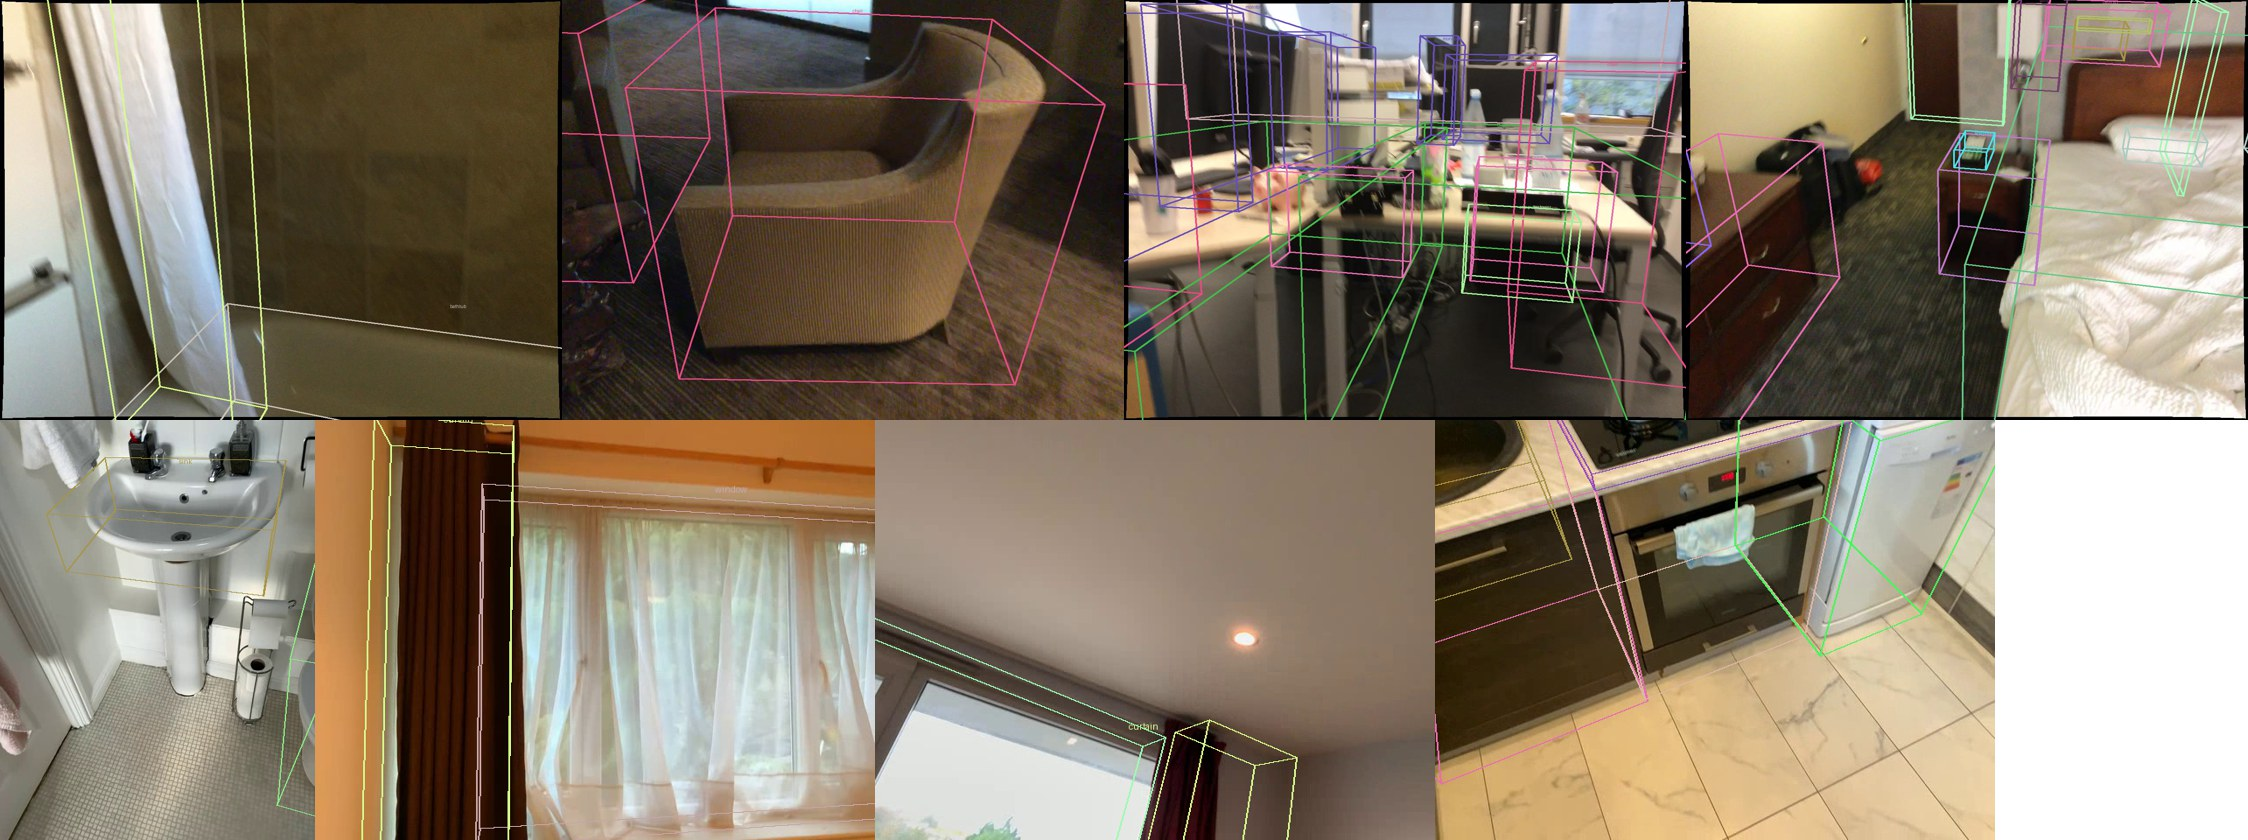
\includegraphics[width=\linewidth]{vggt-det-training-data-overlay.jpg}
\caption{Ground-truth boxes projected into the images with the stored alignment matrix, pose and intrinsics.
Top: ScanNet. Bottom: ARKitScenes after the correction.}
\label{fig:vggtdet-overlay}
\end{figure}

\subsection{Corrections}
\label{sec:vggtdet-data-fix}

\paragraph{Origin.}
For each ARKitScenes scene the alignment matrix gets an extra translation that moves the mean $x$, $y$ of the
points to 0 and their 2nd $z$ percentile (the floor) to 0; the boxes move with it. The median shift is 0.85,
1.87 and 1.23\,m in $x$, $y$ and $z$. The rotation is untouched. Box centres expressed in the scene's world
frame, and hence in every camera's frame, change by less than $10^{-14}$\,m, and sizes do not change.

\paragraph{Focal length.}
Portrait scenes whose focal length is below 0.72 of the long image side (the camera's true value is 0.82 to
0.85) get it multiplied by height over width. This applies to 1,031 of 2,267 training scenes and 265 of 562
validation scenes. Applying either correction a second time changes nothing.

\paragraph{Scope.}
The corrections are applied to the ARKitScenes training and validation files of the 63-class detector and are
built into the two converters that write such files. The files used for inference on Reason-190K and
VSI-Bench keep the first-camera origin on purpose, because the downstream code expects the detections in that
frame. Their portrait focal lengths are still too small; the detector does not read them, but the converter
that writes them (\texttt{build\_arkit\_inputs.py}) should scale by the long image side.
; needs \usepackage{booktabs} and \usepackage{graphicx}.
% Figure file: vggt-det-training-data-overlay.jpg (same folder).
% Data: vggtdet_es56/data/scannet/scannet_infos_train_vsi63.pkl (958 scenes),
%       vggtdet_es56/data/arkit_r190k/arkit_infos_{train,val}_vsi63.pkl (2,267 / 562 scenes).
% Sources: vggtdet_es56/code/tools/vsi63/check_frames_{static,pipeline,model,overlay}.py, scannet_frame.py;
%          results in vggtdet_es56/runs/frame_check/{static,static_after,pipeline,pipeline_after,model}.json.
% Static checks: 150 random scenes per dataset. Pipeline check: 60 random training samples per dataset.

\section{Training data for VGG-T-Det: one box frame for ScanNet and ARKitScenes}
\label{sec:vggtdet-data}

\paragraph{Question.}
VGG-T-Det is fine-tuned on EmbodiedScan boxes of ScanNet (958 scenes) and ARKitScenes (2,267 scenes). The
ScanNet files come from the original VGG-T-Det release, the ARKitScenes files from our own converter. The two
must describe boxes in the same way, or the detector is trained on contradictory targets. We checked this with
several independent tests, each run identically on both datasets so that ScanNet's numbers are the reference.

\paragraph{What the detector's targets depend on.}
The head predicts a box centre in the frame of the first input image and maps it to the scene's aligned frame
with (alignment matrix) $\times$ (pose of the first image). Sizes are predicted directly along the aligned
frame's axes. The targets therefore depend on the rotation of the aligned frame (which way is up, whether the
walls lie on $x$ and $y$), the camera convention of the poses, the metric scale, and the box definition
(gravity centre, axis-aligned size). They do not depend on where the aligned frame's origin is: moving the
origin moves the alignment matrix and the boxes together, and the centre in the first image's frame stays the
same. The stored camera intrinsics are not used by the detector, which takes them from VGGT.

\paragraph{Result.}
The ARKitScenes boxes already agreed with ScanNet in everything the targets depend on. Two things differed,
and neither changed the targets:
\begin{itemize}
\item \textbf{Origin.} ScanNet's aligned frame has the floor at $z=0$ and the mean $x$, $y$ of the scene at 0.
The ARKitScenes files put the origin at the first camera of the trajectory, so the floor was at about
$-1.2$\,m.
\item \textbf{Focal length of portrait videos.} The converter scaled the sensor focal length by image width
over sensor width, which is correct for landscape videos and 0.75 times too small for portrait ones
(398 instead of 531 pixels for a $480\times640$ image). This affected 1,031 of the 2,267 training scenes.
\end{itemize}
Both are now corrected in the ARKitScenes training and validation files (Section~\ref{sec:vggtdet-data-fix}).
Checkpoints trained before the correction remain valid, because the targets are unchanged.

\subsection{Size of the training data}
\label{sec:vggtdet-data-size}

Table~\ref{tab:vggtdet-size} counts the scenes and boxes of the 65-class detector. ScanNet and ARKitScenes use
the EmbodiedScan boxes, ScanNet++ its own annotations. The ARKitScenes and ScanNet++ files include the scenes
built from the raw downloads (\texttt{*\_vsi65\_full.pkl}); before those were added there were 4,272 scenes and
79,670 boxes (ARKitScenes 2,267 / 562 scenes and 39,414 / 9,663 boxes, ScanNet++ 218 / 24 scenes and 7,139 / 742
boxes). Eleven more ARKitScenes training scenes were built but left out (ten with fewer than 42 frames, one without
a box of the 65 classes), and 605 downloaded ScanNet++ scenes lack camera poses. During training ARKitScenes is
validated on a subset of 187 scenes with 3,306 boxes.

\begin{table}[t]
\centering
\caption{Scenes and boxes of the 65-class VGG-T-Det training data (train / validation).}
\label{tab:vggtdet-size}
\begin{tabular}{lrrrrrr}
\toprule
 & \multicolumn{3}{c}{Scenes} & \multicolumn{3}{c}{Boxes} \\
\cmidrule(lr){2-4}\cmidrule(lr){5-7}
Dataset & Train & Val & Total & Train & Val & Total \\
\midrule
ScanNet (EmbodiedScan)     &   958 &   243 & 1,201 & 18,214 &  4,498 &  22,712 \\
ARKitScenes (EmbodiedScan) & 3,587 &   899 & 4,486 & 59,780 & 14,866 &  74,646 \\
ScanNet++                  &   227 &    24 &   251 &  7,543 &    742 &   8,285 \\
\midrule
Total                      & 4,701 & 1,237 & 5,938 & 85,537 & 20,106 & 105,643 \\
\bottomrule
\end{tabular}
\end{table}

\subsection{Checks on the stored files}

\paragraph{Boxes against points.}
Each scene has a point cloud in its raw frame. We move it to the aligned frame and count the points inside each
box. A consistent frame gives full boxes as stored and emptier boxes after any deliberately wrong transform
(Table~\ref{tab:vggtdet-occ}). In both datasets nearly every box holds points as stored, and every wrong
variant loses between a quarter and all of them. For boxes at least twice as long as wide, the points around
the box spread along the box's long side in 98.1\% (ScanNet, 880 boxes) and 97.7\% (ARKitScenes, 745 boxes) of
cases, so $x$ and $y$ sizes are not exchanged.

\begin{table}[t]
\centering
\caption{Boxes against points in the aligned frame (150 scenes per dataset; 2,784 ScanNet and 2,578
ARKitScenes boxes; ARKitScenes after the origin correction). First row: share of boxes holding at least 10
points. Other rows: number of points inside all boxes after a wrong transform, relative to the stored boxes.}
\label{tab:vggtdet-occ}
\begin{tabular}{lrr}
\toprule
 & ScanNet & ARKitScenes \\
\midrule
Boxes with $\geq 10$ points, as stored      & 98.5\% & 99.8\% \\
\midrule
Points not moved to the aligned frame       & 0.05 & 0.12 \\
Boxes turned $90^\circ$ about $z$           & 0.34 & 0.33 \\
Boxes flipped in $z$                        & 0.08 & 0.00 \\
Centre read as bottom of the box            & 0.66 & 0.78 \\
Centre read as top of the box               & 0.58 & 0.55 \\
$x$ and $y$ sizes exchanged                 & 0.59 & 0.64 \\
\bottomrule
\end{tabular}
\end{table}

\paragraph{Up direction, walls, cameras.}
Table~\ref{tab:vggtdet-frame} lists the remaining properties of the frame. In both datasets $z$ is up, the
images are upright, the cameras are about 1.4 to 1.5\,m above the floor, and the walls lie on $x$ and $y$. The
wall test turns the point cloud about $z$ and looks for the turn that makes the $x$ and $y$ histograms
sharpest; this turn is within $3^\circ$ of zero in 97\% and 94\% of scenes.

\paragraph{Camera convention.}
We project the coloured points into the images with the stored pose and intrinsics, keep the nearest point
per $8\times8$ pixel cell, and correlate point and image brightness. The stored convention (camera-to-world,
OpenCV axes) gives 0.71 on ScanNet and 0.74 on ARKitScenes; an OpenGL camera or an inverted pose gives about
zero on both. This test found the focal-length error: portrait ARKitScenes images scored 0.41 as stored and
0.77 with the focal length multiplied by $4/3$, while landscape images scored 0.71 as stored.

\begin{table}[t]
\centering
\caption{Frame properties (150 scenes per dataset). ARKitScenes values that changed with the correction are
given as before $\rightarrow$ after.}
\label{tab:vggtdet-frame}
\begin{tabular}{lrr}
\toprule
 & ScanNet & ARKitScenes \\
\midrule
Image-up direction, mean $z$ component          & 0.88 & 0.84 \\
Scenes with upright images                       & 100\% & 100\% \\
Frames rolled by more than $45^\circ$            & 0.02\% & 0.07\% \\
Camera height above the floor (median)           & 1.38\,m & 1.48\,m \\
Walls within $3^\circ$ of $x$ / $y$              & 97\% & 94\% \\
Brightness correlation, stored camera            & 0.71 & 0.51 $\rightarrow$ 0.74 \\
Brightness correlation, OpenGL camera            & $-0.01$ & $-0.01$ \\
Brightness correlation, inverted pose            & 0.15 & 0.00 \\
Floor height in the aligned frame (median)       & $-0.04$\,m & $-1.22 \rightarrow 0.00$\,m \\
\bottomrule
\end{tabular}
\end{table}

\paragraph{Sizes per class.}
For the 18 classes with at least 30 boxes in both samples, the per-class medians agree between the datasets:
the correlation over classes is 0.93 for height, 0.84 for the long side, 0.97 for the short side and 0.95 for
the centre height above the floor. Height in one dataset against the long side in the other gives 0.30. The
scale is metric in both and the vertical axis is the same.

\subsection{Check on what the model receives}

The same tests were run on samples taken from the real training pipeline, after the step that turns the
aligned frame so that $+y$ is the wall direction nearest the first image's viewing direction
(60 samples per dataset; 1,116 ScanNet and 1,047 ARKitScenes boxes). The points arrive in the first image's
frame and the boxes in the aligned frame; we applied the matrix the head uses to the points. With it, 98.1\%
(ScanNet) and 99.9\% (ARKitScenes) of boxes hold at least 10 points; leaving out either the pose or the
alignment matrix leaves 4--10\% of the points inside the boxes. The first image looks within $45^\circ$ of
$+y$ in every sample of both datasets (median $17^\circ$ and $16^\circ$ off). The box centres seen from the
first image have similar ranges in both datasets, and for ARKitScenes they are identical before and after the
origin correction.

\subsection{Check with a detector trained on ScanNet only}

A detector that has only seen ScanNet carries ScanNet's box convention. If the ARKitScenes frame agrees, its
boxes on ARKitScenes must land on the ARKitScenes ground truth, and wrong transforms of its boxes must destroy
the overlap just as they do on ScanNet. Table~\ref{tab:vggtdet-model} shows this. The overlap on ARKitScenes
is lower, as expected for an unseen dataset, but a quarter turn, a flip in $z$, or reading the centre as the
bottom or top of the box reduces it in the same way.

\begin{table}[t]
\centering
\caption{Mean IoU between boxes of the ScanNet-only detector (score $\geq 0.3$) and the nearest ground-truth
box of the same class (15,163 pairs on ScanNet, 10,500 on ARKitScenes), as predicted and after wrong
transforms of the predictions.}
\label{tab:vggtdet-model}
\begin{tabular}{lrr}
\toprule
 & ScanNet & ARKitScenes \\
\midrule
As predicted                         & 0.41 & 0.21 \\
Turned $90^\circ$ about $z$          & 0.01 & 0.00 \\
Flipped in $z$                       & 0.01 & 0.04 \\
Centre read as bottom of the box     & 0.19 & 0.13 \\
Centre read as top of the box        & 0.18 & 0.10 \\
\bottomrule
\end{tabular}
\end{table}

\paragraph{An offset that is not a frame error.}
On ARKitScenes the ScanNet-only detector places its boxes a median of 0.16\,m too far along the first image's
viewing direction (ScanNet: 0.01\,m). The offset is constant with distance (slope 1.01), so it is not a scale
error. To decide whether the ground truth or the model is off, we moved the stored camera position in steps of
5\,cm along its three axes and repeated the brightness test. On both datasets the correlation is highest at
zero shift in all three directions (ScanNet 0.64, ARKitScenes 0.63, about 350 images each) and falls on either
side. The stored poses, images and points therefore agree, and the offset is a bias of the ScanNet-trained
model on ARKitScenes images, which fine-tuning on ARKitScenes is meant to remove.

\subsection{Visual check}

Figure~\ref{fig:vggtdet-overlay} draws the stored boxes into the images. The boxes sit on the objects in both
datasets, including portrait ARKitScenes images with the corrected focal length.

\begin{figure}[t]
\centering
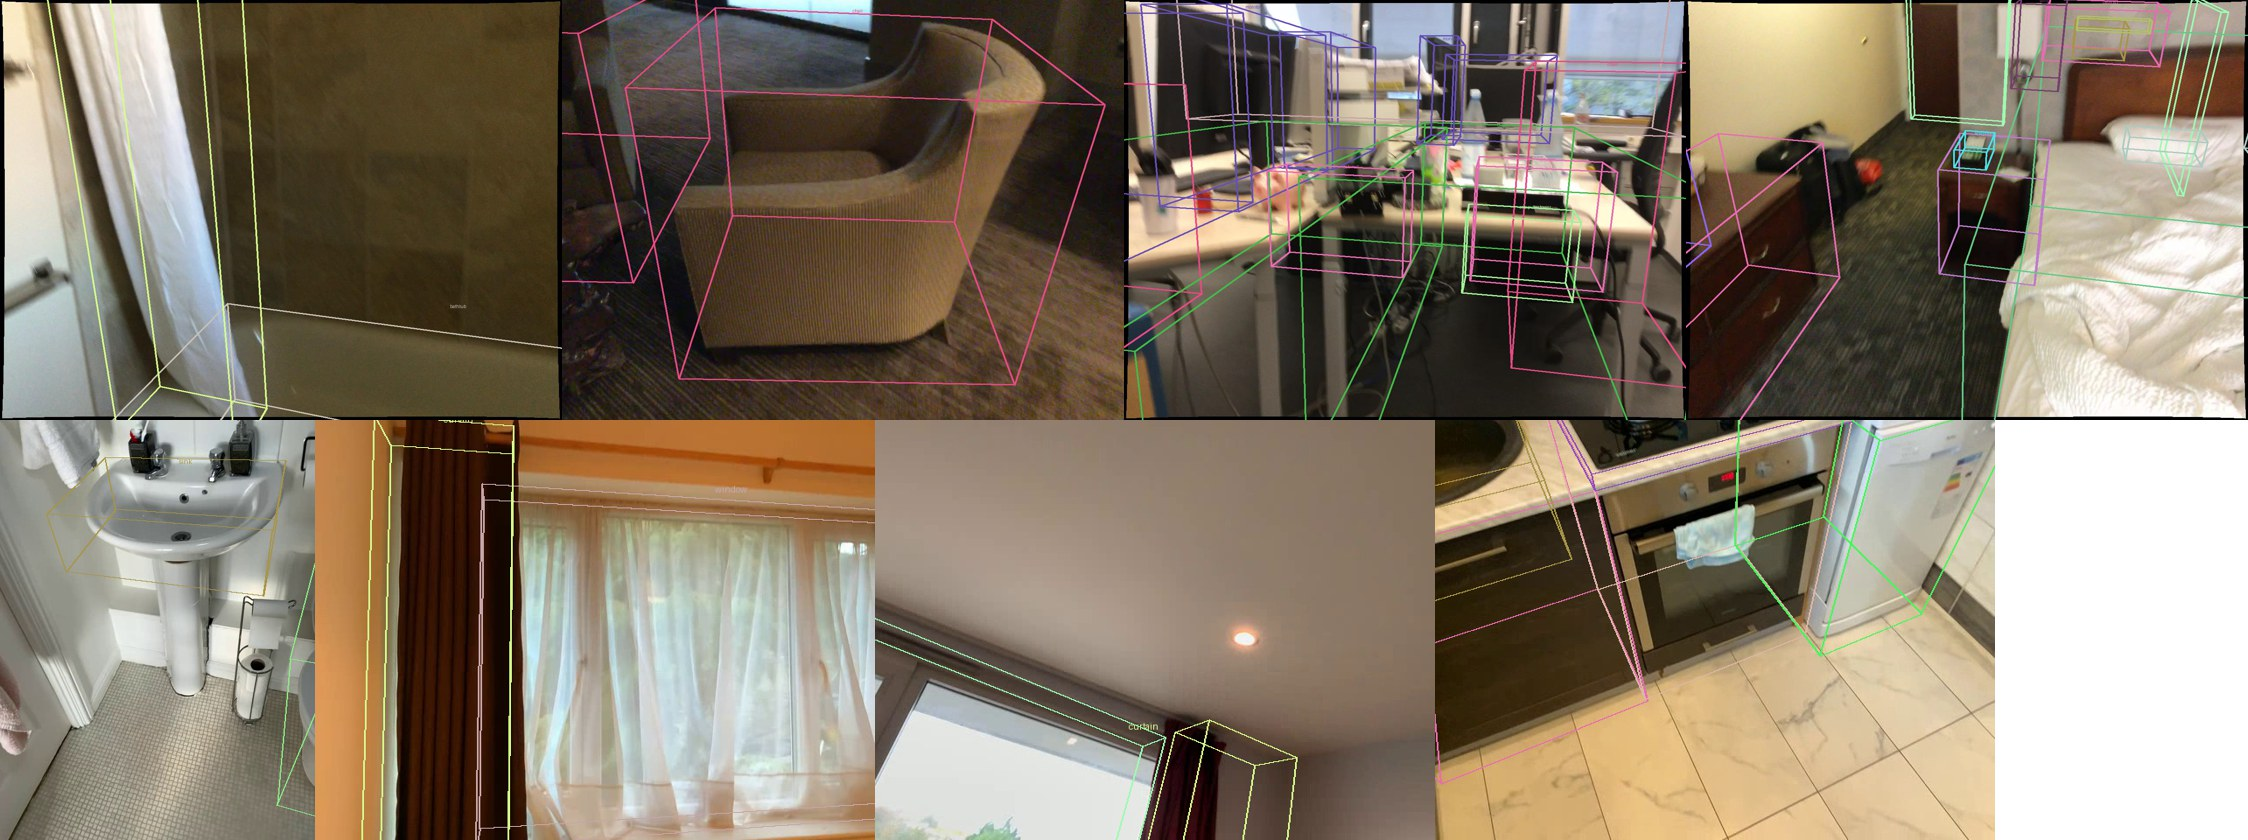
\includegraphics[width=\linewidth]{vggt-det-training-data-overlay.jpg}
\caption{Ground-truth boxes projected into the images with the stored alignment matrix, pose and intrinsics.
Top: ScanNet. Bottom: ARKitScenes after the correction.}
\label{fig:vggtdet-overlay}
\end{figure}

\subsection{Corrections}
\label{sec:vggtdet-data-fix}

\paragraph{Origin.}
For each ARKitScenes scene the alignment matrix gets an extra translation that moves the mean $x$, $y$ of the
points to 0 and their 2nd $z$ percentile (the floor) to 0; the boxes move with it. The median shift is 0.85,
1.87 and 1.23\,m in $x$, $y$ and $z$. The rotation is untouched. Box centres expressed in the scene's world
frame, and hence in every camera's frame, change by less than $10^{-14}$\,m, and sizes do not change.

\paragraph{Focal length.}
Portrait scenes whose focal length is below 0.72 of the long image side (the camera's true value is 0.82 to
0.85) get it multiplied by height over width. This applies to 1,031 of 2,267 training scenes and 265 of 562
validation scenes. Applying either correction a second time changes nothing.

\paragraph{Scope.}
The corrections are applied to the ARKitScenes training and validation files of the 63-class detector and are
built into the two converters that write such files. The files used for inference on Reason-190K and
VSI-Bench keep the first-camera origin on purpose, because the downstream code expects the detections in that
frame. Their portrait focal lengths are still too small; the detector does not read them, but the converter
that writes them (\texttt{build\_arkit\_inputs.py}) should scale by the long image side.
; needs \usepackage{booktabs} and \usepackage{graphicx}.
% Figure file: vggt-det-training-data-overlay.jpg (same folder).
% Data: vggtdet_es56/data/scannet/scannet_infos_train_vsi63.pkl (958 scenes),
%       vggtdet_es56/data/arkit_r190k/arkit_infos_{train,val}_vsi63.pkl (2,267 / 562 scenes).
% Sources: vggtdet_es56/code/tools/vsi63/check_frames_{static,pipeline,model,overlay}.py, scannet_frame.py;
%          results in vggtdet_es56/runs/frame_check/{static,static_after,pipeline,pipeline_after,model}.json.
% Static checks: 150 random scenes per dataset. Pipeline check: 60 random training samples per dataset.

\section{Training data for VGG-T-Det: one box frame for ScanNet and ARKitScenes}
\label{sec:vggtdet-data}

\paragraph{Question.}
VGG-T-Det is fine-tuned on EmbodiedScan boxes of ScanNet (958 scenes) and ARKitScenes (2,267 scenes). The
ScanNet files come from the original VGG-T-Det release, the ARKitScenes files from our own converter. The two
must describe boxes in the same way, or the detector is trained on contradictory targets. We checked this with
several independent tests, each run identically on both datasets so that ScanNet's numbers are the reference.

\paragraph{What the detector's targets depend on.}
The head predicts a box centre in the frame of the first input image and maps it to the scene's aligned frame
with (alignment matrix) $\times$ (pose of the first image). Sizes are predicted directly along the aligned
frame's axes. The targets therefore depend on the rotation of the aligned frame (which way is up, whether the
walls lie on $x$ and $y$), the camera convention of the poses, the metric scale, and the box definition
(gravity centre, axis-aligned size). They do not depend on where the aligned frame's origin is: moving the
origin moves the alignment matrix and the boxes together, and the centre in the first image's frame stays the
same. The stored camera intrinsics are not used by the detector, which takes them from VGGT.

\paragraph{Result.}
The ARKitScenes boxes already agreed with ScanNet in everything the targets depend on. Two things differed,
and neither changed the targets:
\begin{itemize}
\item \textbf{Origin.} ScanNet's aligned frame has the floor at $z=0$ and the mean $x$, $y$ of the scene at 0.
The ARKitScenes files put the origin at the first camera of the trajectory, so the floor was at about
$-1.2$\,m.
\item \textbf{Focal length of portrait videos.} The converter scaled the sensor focal length by image width
over sensor width, which is correct for landscape videos and 0.75 times too small for portrait ones
(398 instead of 531 pixels for a $480\times640$ image). This affected 1,031 of the 2,267 training scenes.
\end{itemize}
Both are now corrected in the ARKitScenes training and validation files (Section~\ref{sec:vggtdet-data-fix}).
Checkpoints trained before the correction remain valid, because the targets are unchanged.

\subsection{Size of the training data}
\label{sec:vggtdet-data-size}

Table~\ref{tab:vggtdet-size} counts the scenes and boxes of the 65-class detector. ScanNet and ARKitScenes use
the EmbodiedScan boxes, ScanNet++ its own annotations. The ARKitScenes and ScanNet++ files include the scenes
built from the raw downloads (\texttt{*\_vsi65\_full.pkl}); before those were added there were 4,272 scenes and
79,670 boxes (ARKitScenes 2,267 / 562 scenes and 39,414 / 9,663 boxes, ScanNet++ 218 / 24 scenes and 7,139 / 742
boxes). Eleven more ARKitScenes training scenes were built but left out (ten with fewer than 42 frames, one without
a box of the 65 classes), and 605 downloaded ScanNet++ scenes lack camera poses. During training ARKitScenes is
validated on a subset of 187 scenes with 3,306 boxes.

\begin{table}[t]
\centering
\caption{Scenes and boxes of the 65-class VGG-T-Det training data (train / validation).}
\label{tab:vggtdet-size}
\begin{tabular}{lrrrrrr}
\toprule
 & \multicolumn{3}{c}{Scenes} & \multicolumn{3}{c}{Boxes} \\
\cmidrule(lr){2-4}\cmidrule(lr){5-7}
Dataset & Train & Val & Total & Train & Val & Total \\
\midrule
ScanNet (EmbodiedScan)     &   958 &   243 & 1,201 & 18,214 &  4,498 &  22,712 \\
ARKitScenes (EmbodiedScan) & 3,587 &   899 & 4,486 & 59,780 & 14,866 &  74,646 \\
ScanNet++                  &   227 &    24 &   251 &  7,543 &    742 &   8,285 \\
\midrule
Total                      & 4,701 & 1,237 & 5,938 & 85,537 & 20,106 & 105,643 \\
\bottomrule
\end{tabular}
\end{table}

\subsection{Checks on the stored files}

\paragraph{Boxes against points.}
Each scene has a point cloud in its raw frame. We move it to the aligned frame and count the points inside each
box. A consistent frame gives full boxes as stored and emptier boxes after any deliberately wrong transform
(Table~\ref{tab:vggtdet-occ}). In both datasets nearly every box holds points as stored, and every wrong
variant loses between a quarter and all of them. For boxes at least twice as long as wide, the points around
the box spread along the box's long side in 98.1\% (ScanNet, 880 boxes) and 97.7\% (ARKitScenes, 745 boxes) of
cases, so $x$ and $y$ sizes are not exchanged.

\begin{table}[t]
\centering
\caption{Boxes against points in the aligned frame (150 scenes per dataset; 2,784 ScanNet and 2,578
ARKitScenes boxes; ARKitScenes after the origin correction). First row: share of boxes holding at least 10
points. Other rows: number of points inside all boxes after a wrong transform, relative to the stored boxes.}
\label{tab:vggtdet-occ}
\begin{tabular}{lrr}
\toprule
 & ScanNet & ARKitScenes \\
\midrule
Boxes with $\geq 10$ points, as stored      & 98.5\% & 99.8\% \\
\midrule
Points not moved to the aligned frame       & 0.05 & 0.12 \\
Boxes turned $90^\circ$ about $z$           & 0.34 & 0.33 \\
Boxes flipped in $z$                        & 0.08 & 0.00 \\
Centre read as bottom of the box            & 0.66 & 0.78 \\
Centre read as top of the box               & 0.58 & 0.55 \\
$x$ and $y$ sizes exchanged                 & 0.59 & 0.64 \\
\bottomrule
\end{tabular}
\end{table}

\paragraph{Up direction, walls, cameras.}
Table~\ref{tab:vggtdet-frame} lists the remaining properties of the frame. In both datasets $z$ is up, the
images are upright, the cameras are about 1.4 to 1.5\,m above the floor, and the walls lie on $x$ and $y$. The
wall test turns the point cloud about $z$ and looks for the turn that makes the $x$ and $y$ histograms
sharpest; this turn is within $3^\circ$ of zero in 97\% and 94\% of scenes.

\paragraph{Camera convention.}
We project the coloured points into the images with the stored pose and intrinsics, keep the nearest point
per $8\times8$ pixel cell, and correlate point and image brightness. The stored convention (camera-to-world,
OpenCV axes) gives 0.71 on ScanNet and 0.74 on ARKitScenes; an OpenGL camera or an inverted pose gives about
zero on both. This test found the focal-length error: portrait ARKitScenes images scored 0.41 as stored and
0.77 with the focal length multiplied by $4/3$, while landscape images scored 0.71 as stored.

\begin{table}[t]
\centering
\caption{Frame properties (150 scenes per dataset). ARKitScenes values that changed with the correction are
given as before $\rightarrow$ after.}
\label{tab:vggtdet-frame}
\begin{tabular}{lrr}
\toprule
 & ScanNet & ARKitScenes \\
\midrule
Image-up direction, mean $z$ component          & 0.88 & 0.84 \\
Scenes with upright images                       & 100\% & 100\% \\
Frames rolled by more than $45^\circ$            & 0.02\% & 0.07\% \\
Camera height above the floor (median)           & 1.38\,m & 1.48\,m \\
Walls within $3^\circ$ of $x$ / $y$              & 97\% & 94\% \\
Brightness correlation, stored camera            & 0.71 & 0.51 $\rightarrow$ 0.74 \\
Brightness correlation, OpenGL camera            & $-0.01$ & $-0.01$ \\
Brightness correlation, inverted pose            & 0.15 & 0.00 \\
Floor height in the aligned frame (median)       & $-0.04$\,m & $-1.22 \rightarrow 0.00$\,m \\
\bottomrule
\end{tabular}
\end{table}

\paragraph{Sizes per class.}
For the 18 classes with at least 30 boxes in both samples, the per-class medians agree between the datasets:
the correlation over classes is 0.93 for height, 0.84 for the long side, 0.97 for the short side and 0.95 for
the centre height above the floor. Height in one dataset against the long side in the other gives 0.30. The
scale is metric in both and the vertical axis is the same.

\subsection{Check on what the model receives}

The same tests were run on samples taken from the real training pipeline, after the step that turns the
aligned frame so that $+y$ is the wall direction nearest the first image's viewing direction
(60 samples per dataset; 1,116 ScanNet and 1,047 ARKitScenes boxes). The points arrive in the first image's
frame and the boxes in the aligned frame; we applied the matrix the head uses to the points. With it, 98.1\%
(ScanNet) and 99.9\% (ARKitScenes) of boxes hold at least 10 points; leaving out either the pose or the
alignment matrix leaves 4--10\% of the points inside the boxes. The first image looks within $45^\circ$ of
$+y$ in every sample of both datasets (median $17^\circ$ and $16^\circ$ off). The box centres seen from the
first image have similar ranges in both datasets, and for ARKitScenes they are identical before and after the
origin correction.

\subsection{Check with a detector trained on ScanNet only}

A detector that has only seen ScanNet carries ScanNet's box convention. If the ARKitScenes frame agrees, its
boxes on ARKitScenes must land on the ARKitScenes ground truth, and wrong transforms of its boxes must destroy
the overlap just as they do on ScanNet. Table~\ref{tab:vggtdet-model} shows this. The overlap on ARKitScenes
is lower, as expected for an unseen dataset, but a quarter turn, a flip in $z$, or reading the centre as the
bottom or top of the box reduces it in the same way.

\begin{table}[t]
\centering
\caption{Mean IoU between boxes of the ScanNet-only detector (score $\geq 0.3$) and the nearest ground-truth
box of the same class (15,163 pairs on ScanNet, 10,500 on ARKitScenes), as predicted and after wrong
transforms of the predictions.}
\label{tab:vggtdet-model}
\begin{tabular}{lrr}
\toprule
 & ScanNet & ARKitScenes \\
\midrule
As predicted                         & 0.41 & 0.21 \\
Turned $90^\circ$ about $z$          & 0.01 & 0.00 \\
Flipped in $z$                       & 0.01 & 0.04 \\
Centre read as bottom of the box     & 0.19 & 0.13 \\
Centre read as top of the box        & 0.18 & 0.10 \\
\bottomrule
\end{tabular}
\end{table}

\paragraph{An offset that is not a frame error.}
On ARKitScenes the ScanNet-only detector places its boxes a median of 0.16\,m too far along the first image's
viewing direction (ScanNet: 0.01\,m). The offset is constant with distance (slope 1.01), so it is not a scale
error. To decide whether the ground truth or the model is off, we moved the stored camera position in steps of
5\,cm along its three axes and repeated the brightness test. On both datasets the correlation is highest at
zero shift in all three directions (ScanNet 0.64, ARKitScenes 0.63, about 350 images each) and falls on either
side. The stored poses, images and points therefore agree, and the offset is a bias of the ScanNet-trained
model on ARKitScenes images, which fine-tuning on ARKitScenes is meant to remove.

\subsection{Visual check}

Figure~\ref{fig:vggtdet-overlay} draws the stored boxes into the images. The boxes sit on the objects in both
datasets, including portrait ARKitScenes images with the corrected focal length.

\begin{figure}[t]
\centering
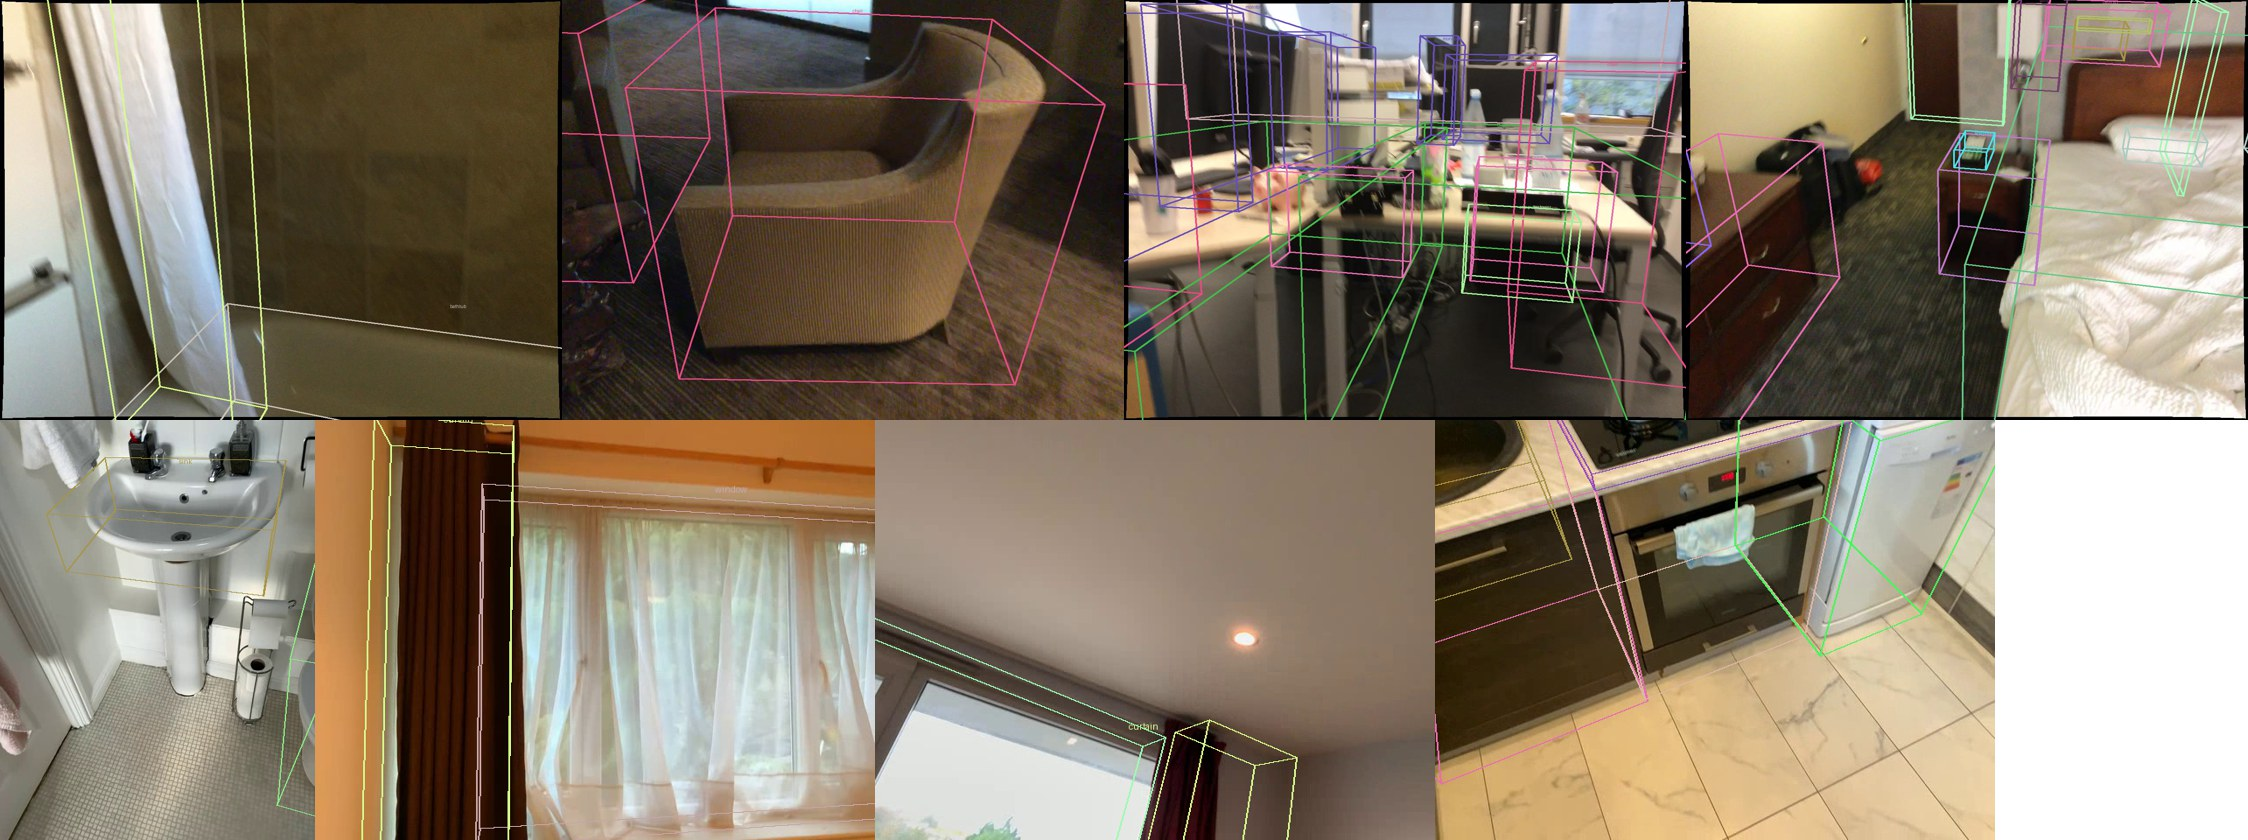
\includegraphics[width=\linewidth]{vggt-det-training-data-overlay.jpg}
\caption{Ground-truth boxes projected into the images with the stored alignment matrix, pose and intrinsics.
Top: ScanNet. Bottom: ARKitScenes after the correction.}
\label{fig:vggtdet-overlay}
\end{figure}

\subsection{Corrections}
\label{sec:vggtdet-data-fix}

\paragraph{Origin.}
For each ARKitScenes scene the alignment matrix gets an extra translation that moves the mean $x$, $y$ of the
points to 0 and their 2nd $z$ percentile (the floor) to 0; the boxes move with it. The median shift is 0.85,
1.87 and 1.23\,m in $x$, $y$ and $z$. The rotation is untouched. Box centres expressed in the scene's world
frame, and hence in every camera's frame, change by less than $10^{-14}$\,m, and sizes do not change.

\paragraph{Focal length.}
Portrait scenes whose focal length is below 0.72 of the long image side (the camera's true value is 0.82 to
0.85) get it multiplied by height over width. This applies to 1,031 of 2,267 training scenes and 265 of 562
validation scenes. Applying either correction a second time changes nothing.

\paragraph{Scope.}
The corrections are applied to the ARKitScenes training and validation files of the 63-class detector and are
built into the two converters that write such files. The files used for inference on Reason-190K and
VSI-Bench keep the first-camera origin on purpose, because the downstream code expects the detections in that
frame. Their portrait focal lengths are still too small; the detector does not read them, but the converter
that writes them (\texttt{build\_arkit\_inputs.py}) should scale by the long image side.

% Claude (no code) on VSI-Bench with the ground-truth scene: Opus 5.5 vs Fable 5.2 (todo 2026.11.18 Exp1-3).
% Fragment for % Claude (no code) on VSI-Bench with the ground-truth scene: Opus 5.5 vs Fable 5.2 (todo 2026.11.18 Exp1-3).
% Fragment for % Claude (no code) on VSI-Bench with the ground-truth scene: Opus 5.5 vs Fable 5.2 (todo 2026.11.18 Exp1-3).
% Fragment for \input{agent}; needs \usepackage{booktabs} and \usepackage{url}.
% Sources: vggtdet_es56/runs/claude_nocode_s3 (build_gt.py, RULES.md, validate.py, score.py; answers in out/ of set gt),
% Opus 5.5 run: 3d-scene-lang/docs/reproduce_exps.md:895.

\section{Language agents without code on the ground-truth scene}
\label{sec:agent}

\paragraph{Setup.}
Each VSI-Bench question is given as text only: the ground-truth object list of its scene (label, centre, size, and
yaw, roll and pitch of each box, in metres and radians), the question and its options; no video. The questions are answered by Claude Code sub-agents
that may use only the Read and Write tools (no code, no calculator), so every computation is done in the model's
own reasoning. A batch holds one question type and at most one question per scene, and each question is answered
from its own text only. All 5,130 questions are answered in 289 batches; we checked that every batch used only
Read and Write.

\paragraph{Fable 5.2 is better than Opus 5.5, on the tasks the boxes do not answer.}
Table~\ref{tab:agent-fable-opus} compares the two models on the 4,378 questions both answered with the same
batching. Fable 5.2 scores 85.0 against 83.0. The gain comes from appearance order ($+9.2$) and route planning
($+8.1$); the geometry tasks are at the ceiling for both models, and room size stays the weak task for both
(about 61--64). On all of VSI-Bench Fable 5.2 reaches 85.2 (full) and 85.0 (debiased), against 84.3 and 84.1.

\begin{table}[t]
\centering
\caption{Claude without code, given the ground-truth scene as text (no video). Accuracy (multiple choice) or
MRA (numeric) per task; ``Overall'' is the mean over the eight tasks. Upper part: the 4,378 questions outside the
debiased ScanNet++ subset, answered with the same batching by both models. Lower part: all of VSI-Bench.}
\label{tab:agent-fable-opus}
\begin{tabular}{lrrr}
\toprule
Task & Opus 5.5 & Fable 5.2 & $\Delta$ \\
\midrule
Appearance order   & 45.2  & 54.4  & $+9.2$ \\
Absolute distance  & 97.2  & 97.0  & $-0.2$ \\
Counting           & 99.3  & 99.3  & $0.0$ \\
Relative direction & 100.0 & 100.0 & $0.0$ \\
Relative distance  & 100.0 & 100.0 & $0.0$ \\
Object size        & 100.0 & 100.0 & $0.0$ \\
Room size          & 62.3  & 61.3  & $-1.0$ \\
Route planning     & 59.9  & 68.0  & $+8.1$ \\
\midrule
Overall (4,378 questions) & 83.0 & \textbf{85.0} & $+2.0$ \\
\midrule
VSI-Bench full (5,130)        & 84.3 & \textbf{85.2} & $+0.9$ \\
VSI-Bench debiased (2,362)    & 84.1 & \textbf{85.0} & $+0.9$ \\
\bottomrule
\end{tabular}
\end{table}

\paragraph{Note on the debiased ScanNet++ questions.}
The remaining 752 questions (debiased ScanNet++) were answered by Opus 5.5 with several questions of the same
scene in one batch, which helps appearance order (81.9); Fable 5.2 answered them one question per scene (63.8).
On these questions Opus 5.5 scores 89.9 and Fable 5.2 85.9, but the comparison is not fair to Fable 5.2, so the
upper part of Table~\ref{tab:agent-fable-opus} leaves them out.

% Code solver on predicted scenes (2026-11-24). Sources (gandalf): 3d-scene-lang/data/scenelang_vsibench_slam/
% oracle_code_lists.py (answers oracle_code_<list>.json), s3_oracle_rows.py in VGGT-SLAM/exps/vsibench_objects (oracle /
% oraclecnt lists), model runs runs/eval_q35vs_gandalf/exp1_s3q_rr_{full,gt_full,oracle_full,oraclecnt_full}_rvs_question,
% mixed answers mix_code_model_oraclecnt.json.
\section{Code written by Claude on predicted scenes}
\label{sec:agent-code}

\paragraph{Setup.}
The code solver (\texttt{oracle.py}, written by Claude) answers a question by computation on the box list alone, with no
model and no video. Counting is the number of boxes with the label; object size is the longest side of the label's first
(best-scoring) box; absolute and relative distance are the closest-point distance between boxes; relative direction uses
the box centres (standing at A, facing B, the side of C from cross and dot products); room size is the area of the
smallest rotated rectangle covering every box in the floor plane. Appearance order and route planning cannot be computed
from boxes and score 0; a question whose named object has no box gets no answer and scores 0. We run it on all 5,130
VSI-Bench questions with these lists (all with the list on every question):
\begin{itemize}
\item \emph{threshold}: the SAM~3 + VGGT-SLAM boxes with score $\geq 0.7$, at estimated or real scale;
\item \emph{oracle}: all SAM~3 + VGGT-SLAM candidates at any score, matched one-to-one to the GT boxes of their label
  (Hungarian on centre distance, in the GT frame at true scale); a pair is kept if the 3D IoU is $\geq 0.1$ or the centres
  are within $\max(0.5\,\mathrm{m},\ 0.5\times$ the GT box's longest side); written at estimated scale;
\item \emph{oraclecnt}: as oracle but without the position check, so each GT object keeps one candidate of its label if
  there is one (94.9\% of the GT objects; oracle keeps 82.3\%); estimated scale;
\item the ground-truth scene, as a reference.
\end{itemize}
The model is the SFT Qwen3.5-4B Exp1 model (\path{sr_vggt_novggt_qwen35_4b_reason190k_mixv2_1_objq/checkpoint-569}) on
the same lists with the video.

\begin{table}[h]
\centering
\caption{Code solver alone on VSI-Bench (MRA or accuracy, \%). Appearance order and route planning are not computable
(0). ``6 tasks'': mean over the six computable tasks.}
\label{tab:agent-code}
\small
\setlength{\tabcolsep}{4pt}
\begin{tabular}{lrrrrrrrrrrr}
\toprule
List & Full & Deb. & App. & Abs. & Count & Rel.\ dir. & Rel.\ dist. & Size & Room & Route & 6 tasks \\
\midrule
GT scene (ref.)                 & 67.8 & 68.0 & -- & 97.4 & 99.0 & 100.0 & 100.0 & 100.0 & 45.8 & -- & 90.4 \\
S3 estimated, threshold         & 35.6 & 34.5 & -- & 37.5 & 53.8 & 49.5 & 52.4 & 52.6 & 39.3 & -- & 47.5 \\
S3 real, threshold (ref.)       & 36.7 & 35.8 & -- & 44.0 & 53.8 & 49.5 & 52.7 & 54.6 & 39.3 & -- & 49.0 \\
S3 estimated, oracle            & 43.7 & 42.3 & -- & 51.2 & 72.6 & 66.8 & 72.1 & 54.7 & 32.2 & -- & 58.3 \\
S3 estimated, oraclecnt         & 50.1 & 49.5 & -- & 57.4 & \textbf{90.5} & 81.7 & 80.0 & 57.8 & 33.4 & -- & 66.8 \\
\bottomrule
\end{tabular}
\end{table}

\paragraph{Code alone.}
Table~\ref{tab:agent-code}. With the threshold list about 1,100 questions get no answer because a named object has no
box (e.g.\ 308 of 834 absolute-distance questions); with oraclecnt only 269 do. On the GT scene the code is at the ceiling
on every geometry task except room size (45.8).

\begin{table}[h]
\centering
\caption{Code solver vs.\ the Exp1 model on the same list (MRA or accuracy, \%). ``Code, else model'': the code's answer
where it has one, otherwise the model's (no box, appearance order, route planning).}
\label{tab:agent-code-model}
\small
\setlength{\tabcolsep}{4pt}
\begin{tabular}{llrrrrrrrrrr}
\toprule
List & Answered by & Full & Deb. & App. & Abs. & Count & Rel.\ dir. & Rel.\ dist. & Size & Room & Route \\
\midrule
threshold & model            & 70.0 & 63.3 & 80.7 & 58.5 & 77.1 & 77.0 & 68.7 & 75.7 & 73.1 & 49.5 \\
threshold & code, else model & 62.0 & 58.6 & 80.7 & 56.5 & 53.8 & \textbf{81.8} & \textbf{69.9} & 64.2 & 39.5 & 49.5 \\
\midrule
oracle    & model            & 71.3 & 64.8 & 81.9 & 61.8 & 79.9 & 77.9 & 70.3 & 75.8 & 72.4 & 50.5 \\
oracle    & code, else model & 67.2 & 63.9 & 81.9 & 62.5 & 72.6 & \textbf{90.8} & \textbf{83.1} & 63.0 & 33.2 & 50.5 \\
\midrule
oraclecnt & model            & 71.8 & 65.5 & 80.9 & 62.5 & 82.3 & 78.0 & 71.5 & 75.8 & 73.2 & 50.0 \\
oraclecnt & code, else model & 68.9 & 66.4 & 80.9 & 62.0 & \textbf{90.5} & \textbf{90.0} & \textbf{84.2} & 60.3 & 33.7 & 50.0 \\
\bottomrule
\end{tabular}
\end{table}

\paragraph{Code vs.\ model.}
Table~\ref{tab:agent-code-model} (estimated scale). On relative direction and relative distance the code is better
whenever the boxes exist (90.0 / 84.2 against 78.0 / 71.5 with oraclecnt), and better even on the threshold list: the model
does not compute this geometry from the boxes reliably. On counting the code is better only with a good list (90.5 against
82.3 with oraclecnt, where the model changes correct counts); on the threshold list the model is far better (77.1 against
53.8), since it corrects bad counts from the video. On object size and room size the model is clearly better: even
GT-picked SAM~3 boxes are too small or too large (size 55--58 from the code), and room size from the box outline is poor
(33--39), while the model uses the video (73). Absolute distance is about the same.

\begin{table}[h]
\centering
\caption{Code and model mixed on the oraclecnt list (MRA or accuracy, \%): the code answers absolute distance,
counting, relative direction and relative distance (2,854 questions); the Exp1 model answers object size, room size and
route planning, and appearance order, which the code cannot compute (2,053), and the 223 code questions whose named object
has no box.}
\label{tab:agent-code-mix}
\small
\setlength{\tabcolsep}{4pt}
\begin{tabular}{lrrrrrrrrrr}
\toprule
 & Full & Deb. & App. & Abs. & Count & Rel.\ dir. & Rel.\ dist. & Size & Room & Route \\
\midrule
Exp1 model only         & 71.8 & 65.5 & 80.9 & 62.5 & 82.3 & 78.0 & 71.5 & 75.8 & 73.2 & 50.0 \\
Mix: code + model       & \textbf{75.8} & \textbf{72.2} & 80.9 & 62.0 & \textbf{90.5} & \textbf{90.0} & \textbf{84.2} & 75.8 & 73.2 & 50.0 \\
$\Delta$                & $+4.0$ & $+6.7$ & $0.0$ & $-0.5$ & $+8.2$ & $+12.0$ & $+12.7$ & $0.0$ & $0.0$ & $0.0$ \\
\bottomrule
\end{tabular}
\end{table}

\paragraph{Mixing code and model.}
Table~\ref{tab:agent-code-mix}: with the oraclecnt list, letting the code answer the four tasks it computes well raises
VSI-Bench from 71.8 to 75.8 (full) and from 65.5 to 72.2 (debiased). Absolute distance is the one code task that is
slightly worse than the model ($-0.5$); answering it with the model too would give about 75.9.
; needs \usepackage{booktabs} and \usepackage{url}.
% Sources: vggtdet_es56/runs/claude_nocode_s3 (build_gt.py, RULES.md, validate.py, score.py; answers in out/ of set gt),
% Opus 5.5 run: 3d-scene-lang/docs/reproduce_exps.md:895.

\section{Language agents without code on the ground-truth scene}
\label{sec:agent}

\paragraph{Setup.}
Each VSI-Bench question is given as text only: the ground-truth object list of its scene (label, centre, size, and
yaw, roll and pitch of each box, in metres and radians), the question and its options; no video. The questions are answered by Claude Code sub-agents
that may use only the Read and Write tools (no code, no calculator), so every computation is done in the model's
own reasoning. A batch holds one question type and at most one question per scene, and each question is answered
from its own text only. All 5,130 questions are answered in 289 batches; we checked that every batch used only
Read and Write.

\paragraph{Fable 5.2 is better than Opus 5.5, on the tasks the boxes do not answer.}
Table~\ref{tab:agent-fable-opus} compares the two models on the 4,378 questions both answered with the same
batching. Fable 5.2 scores 85.0 against 83.0. The gain comes from appearance order ($+9.2$) and route planning
($+8.1$); the geometry tasks are at the ceiling for both models, and room size stays the weak task for both
(about 61--64). On all of VSI-Bench Fable 5.2 reaches 85.2 (full) and 85.0 (debiased), against 84.3 and 84.1.

\begin{table}[t]
\centering
\caption{Claude without code, given the ground-truth scene as text (no video). Accuracy (multiple choice) or
MRA (numeric) per task; ``Overall'' is the mean over the eight tasks. Upper part: the 4,378 questions outside the
debiased ScanNet++ subset, answered with the same batching by both models. Lower part: all of VSI-Bench.}
\label{tab:agent-fable-opus}
\begin{tabular}{lrrr}
\toprule
Task & Opus 5.5 & Fable 5.2 & $\Delta$ \\
\midrule
Appearance order   & 45.2  & 54.4  & $+9.2$ \\
Absolute distance  & 97.2  & 97.0  & $-0.2$ \\
Counting           & 99.3  & 99.3  & $0.0$ \\
Relative direction & 100.0 & 100.0 & $0.0$ \\
Relative distance  & 100.0 & 100.0 & $0.0$ \\
Object size        & 100.0 & 100.0 & $0.0$ \\
Room size          & 62.3  & 61.3  & $-1.0$ \\
Route planning     & 59.9  & 68.0  & $+8.1$ \\
\midrule
Overall (4,378 questions) & 83.0 & \textbf{85.0} & $+2.0$ \\
\midrule
VSI-Bench full (5,130)        & 84.3 & \textbf{85.2} & $+0.9$ \\
VSI-Bench debiased (2,362)    & 84.1 & \textbf{85.0} & $+0.9$ \\
\bottomrule
\end{tabular}
\end{table}

\paragraph{Note on the debiased ScanNet++ questions.}
The remaining 752 questions (debiased ScanNet++) were answered by Opus 5.5 with several questions of the same
scene in one batch, which helps appearance order (81.9); Fable 5.2 answered them one question per scene (63.8).
On these questions Opus 5.5 scores 89.9 and Fable 5.2 85.9, but the comparison is not fair to Fable 5.2, so the
upper part of Table~\ref{tab:agent-fable-opus} leaves them out.

% Code solver on predicted scenes (2026-11-24). Sources (gandalf): 3d-scene-lang/data/scenelang_vsibench_slam/
% oracle_code_lists.py (answers oracle_code_<list>.json), s3_oracle_rows.py in VGGT-SLAM/exps/vsibench_objects (oracle /
% oraclecnt lists), model runs runs/eval_q35vs_gandalf/exp1_s3q_rr_{full,gt_full,oracle_full,oraclecnt_full}_rvs_question,
% mixed answers mix_code_model_oraclecnt.json.
\section{Code written by Claude on predicted scenes}
\label{sec:agent-code}

\paragraph{Setup.}
The code solver (\texttt{oracle.py}, written by Claude) answers a question by computation on the box list alone, with no
model and no video. Counting is the number of boxes with the label; object size is the longest side of the label's first
(best-scoring) box; absolute and relative distance are the closest-point distance between boxes; relative direction uses
the box centres (standing at A, facing B, the side of C from cross and dot products); room size is the area of the
smallest rotated rectangle covering every box in the floor plane. Appearance order and route planning cannot be computed
from boxes and score 0; a question whose named object has no box gets no answer and scores 0. We run it on all 5,130
VSI-Bench questions with these lists (all with the list on every question):
\begin{itemize}
\item \emph{threshold}: the SAM~3 + VGGT-SLAM boxes with score $\geq 0.7$, at estimated or real scale;
\item \emph{oracle}: all SAM~3 + VGGT-SLAM candidates at any score, matched one-to-one to the GT boxes of their label
  (Hungarian on centre distance, in the GT frame at true scale); a pair is kept if the 3D IoU is $\geq 0.1$ or the centres
  are within $\max(0.5\,\mathrm{m},\ 0.5\times$ the GT box's longest side); written at estimated scale;
\item \emph{oraclecnt}: as oracle but without the position check, so each GT object keeps one candidate of its label if
  there is one (94.9\% of the GT objects; oracle keeps 82.3\%); estimated scale;
\item the ground-truth scene, as a reference.
\end{itemize}
The model is the SFT Qwen3.5-4B Exp1 model (\path{sr_vggt_novggt_qwen35_4b_reason190k_mixv2_1_objq/checkpoint-569}) on
the same lists with the video.

\begin{table}[h]
\centering
\caption{Code solver alone on VSI-Bench (MRA or accuracy, \%). Appearance order and route planning are not computable
(0). ``6 tasks'': mean over the six computable tasks.}
\label{tab:agent-code}
\small
\setlength{\tabcolsep}{4pt}
\begin{tabular}{lrrrrrrrrrrr}
\toprule
List & Full & Deb. & App. & Abs. & Count & Rel.\ dir. & Rel.\ dist. & Size & Room & Route & 6 tasks \\
\midrule
GT scene (ref.)                 & 67.8 & 68.0 & -- & 97.4 & 99.0 & 100.0 & 100.0 & 100.0 & 45.8 & -- & 90.4 \\
S3 estimated, threshold         & 35.6 & 34.5 & -- & 37.5 & 53.8 & 49.5 & 52.4 & 52.6 & 39.3 & -- & 47.5 \\
S3 real, threshold (ref.)       & 36.7 & 35.8 & -- & 44.0 & 53.8 & 49.5 & 52.7 & 54.6 & 39.3 & -- & 49.0 \\
S3 estimated, oracle            & 43.7 & 42.3 & -- & 51.2 & 72.6 & 66.8 & 72.1 & 54.7 & 32.2 & -- & 58.3 \\
S3 estimated, oraclecnt         & 50.1 & 49.5 & -- & 57.4 & \textbf{90.5} & 81.7 & 80.0 & 57.8 & 33.4 & -- & 66.8 \\
\bottomrule
\end{tabular}
\end{table}

\paragraph{Code alone.}
Table~\ref{tab:agent-code}. With the threshold list about 1,100 questions get no answer because a named object has no
box (e.g.\ 308 of 834 absolute-distance questions); with oraclecnt only 269 do. On the GT scene the code is at the ceiling
on every geometry task except room size (45.8).

\begin{table}[h]
\centering
\caption{Code solver vs.\ the Exp1 model on the same list (MRA or accuracy, \%). ``Code, else model'': the code's answer
where it has one, otherwise the model's (no box, appearance order, route planning).}
\label{tab:agent-code-model}
\small
\setlength{\tabcolsep}{4pt}
\begin{tabular}{llrrrrrrrrrr}
\toprule
List & Answered by & Full & Deb. & App. & Abs. & Count & Rel.\ dir. & Rel.\ dist. & Size & Room & Route \\
\midrule
threshold & model            & 70.0 & 63.3 & 80.7 & 58.5 & 77.1 & 77.0 & 68.7 & 75.7 & 73.1 & 49.5 \\
threshold & code, else model & 62.0 & 58.6 & 80.7 & 56.5 & 53.8 & \textbf{81.8} & \textbf{69.9} & 64.2 & 39.5 & 49.5 \\
\midrule
oracle    & model            & 71.3 & 64.8 & 81.9 & 61.8 & 79.9 & 77.9 & 70.3 & 75.8 & 72.4 & 50.5 \\
oracle    & code, else model & 67.2 & 63.9 & 81.9 & 62.5 & 72.6 & \textbf{90.8} & \textbf{83.1} & 63.0 & 33.2 & 50.5 \\
\midrule
oraclecnt & model            & 71.8 & 65.5 & 80.9 & 62.5 & 82.3 & 78.0 & 71.5 & 75.8 & 73.2 & 50.0 \\
oraclecnt & code, else model & 68.9 & 66.4 & 80.9 & 62.0 & \textbf{90.5} & \textbf{90.0} & \textbf{84.2} & 60.3 & 33.7 & 50.0 \\
\bottomrule
\end{tabular}
\end{table}

\paragraph{Code vs.\ model.}
Table~\ref{tab:agent-code-model} (estimated scale). On relative direction and relative distance the code is better
whenever the boxes exist (90.0 / 84.2 against 78.0 / 71.5 with oraclecnt), and better even on the threshold list: the model
does not compute this geometry from the boxes reliably. On counting the code is better only with a good list (90.5 against
82.3 with oraclecnt, where the model changes correct counts); on the threshold list the model is far better (77.1 against
53.8), since it corrects bad counts from the video. On object size and room size the model is clearly better: even
GT-picked SAM~3 boxes are too small or too large (size 55--58 from the code), and room size from the box outline is poor
(33--39), while the model uses the video (73). Absolute distance is about the same.

\begin{table}[h]
\centering
\caption{Code and model mixed on the oraclecnt list (MRA or accuracy, \%): the code answers absolute distance,
counting, relative direction and relative distance (2,854 questions); the Exp1 model answers object size, room size and
route planning, and appearance order, which the code cannot compute (2,053), and the 223 code questions whose named object
has no box.}
\label{tab:agent-code-mix}
\small
\setlength{\tabcolsep}{4pt}
\begin{tabular}{lrrrrrrrrrr}
\toprule
 & Full & Deb. & App. & Abs. & Count & Rel.\ dir. & Rel.\ dist. & Size & Room & Route \\
\midrule
Exp1 model only         & 71.8 & 65.5 & 80.9 & 62.5 & 82.3 & 78.0 & 71.5 & 75.8 & 73.2 & 50.0 \\
Mix: code + model       & \textbf{75.8} & \textbf{72.2} & 80.9 & 62.0 & \textbf{90.5} & \textbf{90.0} & \textbf{84.2} & 75.8 & 73.2 & 50.0 \\
$\Delta$                & $+4.0$ & $+6.7$ & $0.0$ & $-0.5$ & $+8.2$ & $+12.0$ & $+12.7$ & $0.0$ & $0.0$ & $0.0$ \\
\bottomrule
\end{tabular}
\end{table}

\paragraph{Mixing code and model.}
Table~\ref{tab:agent-code-mix}: with the oraclecnt list, letting the code answer the four tasks it computes well raises
VSI-Bench from 71.8 to 75.8 (full) and from 65.5 to 72.2 (debiased). Absolute distance is the one code task that is
slightly worse than the model ($-0.5$); answering it with the model too would give about 75.9.
; needs \usepackage{booktabs} and \usepackage{url}.
% Sources: vggtdet_es56/runs/claude_nocode_s3 (build_gt.py, RULES.md, validate.py, score.py; answers in out/ of set gt),
% Opus 5.5 run: 3d-scene-lang/docs/reproduce_exps.md:895.

\section{Language agents without code on the ground-truth scene}
\label{sec:agent}

\paragraph{Setup.}
Each VSI-Bench question is given as text only: the ground-truth object list of its scene (label, centre, size, and
yaw, roll and pitch of each box, in metres and radians), the question and its options; no video. The questions are answered by Claude Code sub-agents
that may use only the Read and Write tools (no code, no calculator), so every computation is done in the model's
own reasoning. A batch holds one question type and at most one question per scene, and each question is answered
from its own text only. All 5,130 questions are answered in 289 batches; we checked that every batch used only
Read and Write.

\paragraph{Fable 5.2 is better than Opus 5.5, on the tasks the boxes do not answer.}
Table~\ref{tab:agent-fable-opus} compares the two models on the 4,378 questions both answered with the same
batching. Fable 5.2 scores 85.0 against 83.0. The gain comes from appearance order ($+9.2$) and route planning
($+8.1$); the geometry tasks are at the ceiling for both models, and room size stays the weak task for both
(about 61--64). On all of VSI-Bench Fable 5.2 reaches 85.2 (full) and 85.0 (debiased), against 84.3 and 84.1.

\begin{table}[t]
\centering
\caption{Claude without code, given the ground-truth scene as text (no video). Accuracy (multiple choice) or
MRA (numeric) per task; ``Overall'' is the mean over the eight tasks. Upper part: the 4,378 questions outside the
debiased ScanNet++ subset, answered with the same batching by both models. Lower part: all of VSI-Bench.}
\label{tab:agent-fable-opus}
\begin{tabular}{lrrr}
\toprule
Task & Opus 5.5 & Fable 5.2 & $\Delta$ \\
\midrule
Appearance order   & 45.2  & 54.4  & $+9.2$ \\
Absolute distance  & 97.2  & 97.0  & $-0.2$ \\
Counting           & 99.3  & 99.3  & $0.0$ \\
Relative direction & 100.0 & 100.0 & $0.0$ \\
Relative distance  & 100.0 & 100.0 & $0.0$ \\
Object size        & 100.0 & 100.0 & $0.0$ \\
Room size          & 62.3  & 61.3  & $-1.0$ \\
Route planning     & 59.9  & 68.0  & $+8.1$ \\
\midrule
Overall (4,378 questions) & 83.0 & \textbf{85.0} & $+2.0$ \\
\midrule
VSI-Bench full (5,130)        & 84.3 & \textbf{85.2} & $+0.9$ \\
VSI-Bench debiased (2,362)    & 84.1 & \textbf{85.0} & $+0.9$ \\
\bottomrule
\end{tabular}
\end{table}

\paragraph{Note on the debiased ScanNet++ questions.}
The remaining 752 questions (debiased ScanNet++) were answered by Opus 5.5 with several questions of the same
scene in one batch, which helps appearance order (81.9); Fable 5.2 answered them one question per scene (63.8).
On these questions Opus 5.5 scores 89.9 and Fable 5.2 85.9, but the comparison is not fair to Fable 5.2, so the
upper part of Table~\ref{tab:agent-fable-opus} leaves them out.

% Code solver on predicted scenes (2026-11-24). Sources (gandalf): 3d-scene-lang/data/scenelang_vsibench_slam/
% oracle_code_lists.py (answers oracle_code_<list>.json), s3_oracle_rows.py in VGGT-SLAM/exps/vsibench_objects (oracle /
% oraclecnt lists), model runs runs/eval_q35vs_gandalf/exp1_s3q_rr_{full,gt_full,oracle_full,oraclecnt_full}_rvs_question,
% mixed answers mix_code_model_oraclecnt.json.
\section{Code written by Claude on predicted scenes}
\label{sec:agent-code}

\paragraph{Setup.}
The code solver (\texttt{oracle.py}, written by Claude) answers a question by computation on the box list alone, with no
model and no video. Counting is the number of boxes with the label; object size is the longest side of the label's first
(best-scoring) box; absolute and relative distance are the closest-point distance between boxes; relative direction uses
the box centres (standing at A, facing B, the side of C from cross and dot products); room size is the area of the
smallest rotated rectangle covering every box in the floor plane. Appearance order and route planning cannot be computed
from boxes and score 0; a question whose named object has no box gets no answer and scores 0. We run it on all 5,130
VSI-Bench questions with these lists (all with the list on every question):
\begin{itemize}
\item \emph{threshold}: the SAM~3 + VGGT-SLAM boxes with score $\geq 0.7$, at estimated or real scale;
\item \emph{oracle}: all SAM~3 + VGGT-SLAM candidates at any score, matched one-to-one to the GT boxes of their label
  (Hungarian on centre distance, in the GT frame at true scale); a pair is kept if the 3D IoU is $\geq 0.1$ or the centres
  are within $\max(0.5\,\mathrm{m},\ 0.5\times$ the GT box's longest side); written at estimated scale;
\item \emph{oraclecnt}: as oracle but without the position check, so each GT object keeps one candidate of its label if
  there is one (94.9\% of the GT objects; oracle keeps 82.3\%); estimated scale;
\item the ground-truth scene, as a reference.
\end{itemize}
The model is the SFT Qwen3.5-4B Exp1 model (\path{sr_vggt_novggt_qwen35_4b_reason190k_mixv2_1_objq/checkpoint-569}) on
the same lists with the video.

\begin{table}[h]
\centering
\caption{Code solver alone on VSI-Bench (MRA or accuracy, \%). Appearance order and route planning are not computable
(0). ``6 tasks'': mean over the six computable tasks.}
\label{tab:agent-code}
\small
\setlength{\tabcolsep}{4pt}
\begin{tabular}{lrrrrrrrrrrr}
\toprule
List & Full & Deb. & App. & Abs. & Count & Rel.\ dir. & Rel.\ dist. & Size & Room & Route & 6 tasks \\
\midrule
GT scene (ref.)                 & 67.8 & 68.0 & -- & 97.4 & 99.0 & 100.0 & 100.0 & 100.0 & 45.8 & -- & 90.4 \\
S3 estimated, threshold         & 35.6 & 34.5 & -- & 37.5 & 53.8 & 49.5 & 52.4 & 52.6 & 39.3 & -- & 47.5 \\
S3 real, threshold (ref.)       & 36.7 & 35.8 & -- & 44.0 & 53.8 & 49.5 & 52.7 & 54.6 & 39.3 & -- & 49.0 \\
S3 estimated, oracle            & 43.7 & 42.3 & -- & 51.2 & 72.6 & 66.8 & 72.1 & 54.7 & 32.2 & -- & 58.3 \\
S3 estimated, oraclecnt         & 50.1 & 49.5 & -- & 57.4 & \textbf{90.5} & 81.7 & 80.0 & 57.8 & 33.4 & -- & 66.8 \\
\bottomrule
\end{tabular}
\end{table}

\paragraph{Code alone.}
Table~\ref{tab:agent-code}. With the threshold list about 1,100 questions get no answer because a named object has no
box (e.g.\ 308 of 834 absolute-distance questions); with oraclecnt only 269 do. On the GT scene the code is at the ceiling
on every geometry task except room size (45.8).

\begin{table}[h]
\centering
\caption{Code solver vs.\ the Exp1 model on the same list (MRA or accuracy, \%). ``Code, else model'': the code's answer
where it has one, otherwise the model's (no box, appearance order, route planning).}
\label{tab:agent-code-model}
\small
\setlength{\tabcolsep}{4pt}
\begin{tabular}{llrrrrrrrrrr}
\toprule
List & Answered by & Full & Deb. & App. & Abs. & Count & Rel.\ dir. & Rel.\ dist. & Size & Room & Route \\
\midrule
threshold & model            & 70.0 & 63.3 & 80.7 & 58.5 & 77.1 & 77.0 & 68.7 & 75.7 & 73.1 & 49.5 \\
threshold & code, else model & 62.0 & 58.6 & 80.7 & 56.5 & 53.8 & \textbf{81.8} & \textbf{69.9} & 64.2 & 39.5 & 49.5 \\
\midrule
oracle    & model            & 71.3 & 64.8 & 81.9 & 61.8 & 79.9 & 77.9 & 70.3 & 75.8 & 72.4 & 50.5 \\
oracle    & code, else model & 67.2 & 63.9 & 81.9 & 62.5 & 72.6 & \textbf{90.8} & \textbf{83.1} & 63.0 & 33.2 & 50.5 \\
\midrule
oraclecnt & model            & 71.8 & 65.5 & 80.9 & 62.5 & 82.3 & 78.0 & 71.5 & 75.8 & 73.2 & 50.0 \\
oraclecnt & code, else model & 68.9 & 66.4 & 80.9 & 62.0 & \textbf{90.5} & \textbf{90.0} & \textbf{84.2} & 60.3 & 33.7 & 50.0 \\
\bottomrule
\end{tabular}
\end{table}

\paragraph{Code vs.\ model.}
Table~\ref{tab:agent-code-model} (estimated scale). On relative direction and relative distance the code is better
whenever the boxes exist (90.0 / 84.2 against 78.0 / 71.5 with oraclecnt), and better even on the threshold list: the model
does not compute this geometry from the boxes reliably. On counting the code is better only with a good list (90.5 against
82.3 with oraclecnt, where the model changes correct counts); on the threshold list the model is far better (77.1 against
53.8), since it corrects bad counts from the video. On object size and room size the model is clearly better: even
GT-picked SAM~3 boxes are too small or too large (size 55--58 from the code), and room size from the box outline is poor
(33--39), while the model uses the video (73). Absolute distance is about the same.

\begin{table}[h]
\centering
\caption{Code and model mixed on the oraclecnt list (MRA or accuracy, \%): the code answers absolute distance,
counting, relative direction and relative distance (2,854 questions); the Exp1 model answers object size, room size and
route planning, and appearance order, which the code cannot compute (2,053), and the 223 code questions whose named object
has no box.}
\label{tab:agent-code-mix}
\small
\setlength{\tabcolsep}{4pt}
\begin{tabular}{lrrrrrrrrrr}
\toprule
 & Full & Deb. & App. & Abs. & Count & Rel.\ dir. & Rel.\ dist. & Size & Room & Route \\
\midrule
Exp1 model only         & 71.8 & 65.5 & 80.9 & 62.5 & 82.3 & 78.0 & 71.5 & 75.8 & 73.2 & 50.0 \\
Mix: code + model       & \textbf{75.8} & \textbf{72.2} & 80.9 & 62.0 & \textbf{90.5} & \textbf{90.0} & \textbf{84.2} & 75.8 & 73.2 & 50.0 \\
$\Delta$                & $+4.0$ & $+6.7$ & $0.0$ & $-0.5$ & $+8.2$ & $+12.0$ & $+12.7$ & $0.0$ & $0.0$ & $0.0$ \\
\bottomrule
\end{tabular}
\end{table}

\paragraph{Mixing code and model.}
Table~\ref{tab:agent-code-mix}: with the oraclecnt list, letting the code answer the four tasks it computes well raises
VSI-Bench from 71.8 to 75.8 (full) and from 65.5 to 72.2 (debiased). Absolute distance is the one code task that is
slightly worse than the model ($-0.5$); answering it with the model too would give about 75.9.

% Claude (no code) on VSI-Bench with the vggt-slam-sam3 scene at estimated scale, score-aware prompt (todo 2026.11.18 Exp1-2-2).
% Fragment for % Claude (no code) on VSI-Bench with the vggt-slam-sam3 scene at estimated scale, score-aware prompt (todo 2026.11.18 Exp1-2-2).
% Fragment for % Claude (no code) on VSI-Bench with the vggt-slam-sam3 scene at estimated scale, score-aware prompt (todo 2026.11.18 Exp1-2-2).
% Fragment for \input{claude}; needs \usepackage{booktabs}. Companion of agent.tex (ground-truth scene, Opus 5.5 vs Fable 5.2).
% Sources: vggtdet_es56/runs/claude_nocode_s3 (build_est.py -> e2/batches, RULES.md, validate.py, score.py; answers in e2/out),
% rows: 3d-scene-lang/data/scenelang_vsibench_slam/rows_s3q_roomdoor_radiator_all5130_full.jsonl.
% Exp1-1-1, Exp1-1-2 (real scale) and Exp1-2-1 (estimated scale, no score instruction) are paused and not reported here.

\section{Language agents without code on predicted scenes}
\label{sec:claude}

\paragraph{Setup.}
We repeat the experiment of Section~\ref{sec:agent} with the ground-truth scene replaced by the scene that
SAM~3 + VGGT-SLAM predicts from the video (Section~\ref{sec:sam3}), at the scale VGGT-SLAM estimates (no
ground-truth scale). For each question the list holds the SAM~3 boxes of the objects the question names
(including ``room door'' and ``radiator''), with box score $\geq 0.7$, as upright axis-aligned boxes
$[x, y, z, d_x, d_y, d_z]$ in the frame of the first camera, each with its score. The prompt states that the boxes
were predicted by a 3D detector from the video, that objects may be missing, duplicated, mislabelled or misplaced
and sizes may be off, and that the score is the detector's confidence: high-score boxes should be trusted, and
typical indoor layouts used where boxes are missing or unreliable (\emph{score-aware}). As before, each question is
given as text only (no video) and answered by Claude Opus~5.5 sub-agents restricted to the Read and Write tools,
one question type per batch and at most one question per scene. All 5,130 questions were answered in 289 batches,
every one with Read and Write only.

\paragraph{Predicted boxes cost 26 points.}
Table~\ref{tab:claude-s3est} compares the result with the ground-truth scene. With predicted boxes Claude reaches
59.2 (full) and 55.9 (debiased), against 85.2 and 85.0 with the ground-truth scene. The loss is largest on the tasks
that need correct metric scale and a complete object list: absolute distance ($-44.6$) and counting ($-43.6$).
Relative direction, relative distance and object size lose 24 to 35 points. Route planning, which uses the
box geometry least, is unchanged. Without the video Claude cannot correct the predicted list, and it stays
about 10 points below the fine-tuned Qwen3.5-4B given the video and the same boxes (69.0 / 62.9).

\begin{table}[t]
\centering
\caption{Claude Opus~5.5 without code, given the scene as text (no video). Accuracy (multiple choice) or MRA
(numeric) per task on all 5,130 VSI-Bench questions; ``Overall'' is the mean over the eight tasks. Predicted:
SAM~3 + VGGT-SLAM boxes at estimated scale with a score per box and a score-aware prompt. Ground truth: the
ground-truth scene, answered by Fable~5.2 under the same batching rules (Table~\ref{tab:agent-fable-opus}; Opus~5.5:
84.3 / 84.1).}
\label{tab:claude-s3est}
\begin{tabular}{lrrr}
\toprule
Task & Predicted & Ground truth & $\Delta$ \\
\midrule
Appearance order   & 36.2 & 56.5  & $-20.3$ \\
Absolute distance  & 52.0 & 96.6  & $-44.6$ \\
Counting           & 55.6 & 99.2  & $-43.6$ \\
Relative direction & 75.9 & 100.0 & $-24.1$ \\
Relative distance  & 65.4 & 100.0 & $-34.6$ \\
Object size        & 68.2 & 100.0 & $-31.8$ \\
Room size          & 52.7 & 63.8  & $-11.1$ \\
Route planning     & 67.5 & 66.0  & $+1.5$ \\
\midrule
VSI-Bench full (5,130)     & 59.2 & 85.2 & $-26.0$ \\
VSI-Bench debiased (2,362) & 55.9 & 85.0 & $-29.1$ \\
\bottomrule
\end{tabular}
\end{table}
; needs \usepackage{booktabs}. Companion of agent.tex (ground-truth scene, Opus 5.5 vs Fable 5.2).
% Sources: vggtdet_es56/runs/claude_nocode_s3 (build_est.py -> e2/batches, RULES.md, validate.py, score.py; answers in e2/out),
% rows: 3d-scene-lang/data/scenelang_vsibench_slam/rows_s3q_roomdoor_radiator_all5130_full.jsonl.
% Exp1-1-1, Exp1-1-2 (real scale) and Exp1-2-1 (estimated scale, no score instruction) are paused and not reported here.

\section{Language agents without code on predicted scenes}
\label{sec:claude}

\paragraph{Setup.}
We repeat the experiment of Section~\ref{sec:agent} with the ground-truth scene replaced by the scene that
SAM~3 + VGGT-SLAM predicts from the video (Section~\ref{sec:sam3}), at the scale VGGT-SLAM estimates (no
ground-truth scale). For each question the list holds the SAM~3 boxes of the objects the question names
(including ``room door'' and ``radiator''), with box score $\geq 0.7$, as upright axis-aligned boxes
$[x, y, z, d_x, d_y, d_z]$ in the frame of the first camera, each with its score. The prompt states that the boxes
were predicted by a 3D detector from the video, that objects may be missing, duplicated, mislabelled or misplaced
and sizes may be off, and that the score is the detector's confidence: high-score boxes should be trusted, and
typical indoor layouts used where boxes are missing or unreliable (\emph{score-aware}). As before, each question is
given as text only (no video) and answered by Claude Opus~5.5 sub-agents restricted to the Read and Write tools,
one question type per batch and at most one question per scene. All 5,130 questions were answered in 289 batches,
every one with Read and Write only.

\paragraph{Predicted boxes cost 26 points.}
Table~\ref{tab:claude-s3est} compares the result with the ground-truth scene. With predicted boxes Claude reaches
59.2 (full) and 55.9 (debiased), against 85.2 and 85.0 with the ground-truth scene. The loss is largest on the tasks
that need correct metric scale and a complete object list: absolute distance ($-44.6$) and counting ($-43.6$).
Relative direction, relative distance and object size lose 24 to 35 points. Route planning, which uses the
box geometry least, is unchanged. Without the video Claude cannot correct the predicted list, and it stays
about 10 points below the fine-tuned Qwen3.5-4B given the video and the same boxes (69.0 / 62.9).

\begin{table}[t]
\centering
\caption{Claude Opus~5.5 without code, given the scene as text (no video). Accuracy (multiple choice) or MRA
(numeric) per task on all 5,130 VSI-Bench questions; ``Overall'' is the mean over the eight tasks. Predicted:
SAM~3 + VGGT-SLAM boxes at estimated scale with a score per box and a score-aware prompt. Ground truth: the
ground-truth scene, answered by Fable~5.2 under the same batching rules (Table~\ref{tab:agent-fable-opus}; Opus~5.5:
84.3 / 84.1).}
\label{tab:claude-s3est}
\begin{tabular}{lrrr}
\toprule
Task & Predicted & Ground truth & $\Delta$ \\
\midrule
Appearance order   & 36.2 & 56.5  & $-20.3$ \\
Absolute distance  & 52.0 & 96.6  & $-44.6$ \\
Counting           & 55.6 & 99.2  & $-43.6$ \\
Relative direction & 75.9 & 100.0 & $-24.1$ \\
Relative distance  & 65.4 & 100.0 & $-34.6$ \\
Object size        & 68.2 & 100.0 & $-31.8$ \\
Room size          & 52.7 & 63.8  & $-11.1$ \\
Route planning     & 67.5 & 66.0  & $+1.5$ \\
\midrule
VSI-Bench full (5,130)     & 59.2 & 85.2 & $-26.0$ \\
VSI-Bench debiased (2,362) & 55.9 & 85.0 & $-29.1$ \\
\bottomrule
\end{tabular}
\end{table}
; needs \usepackage{booktabs}. Companion of agent.tex (ground-truth scene, Opus 5.5 vs Fable 5.2).
% Sources: vggtdet_es56/runs/claude_nocode_s3 (build_est.py -> e2/batches, RULES.md, validate.py, score.py; answers in e2/out),
% rows: 3d-scene-lang/data/scenelang_vsibench_slam/rows_s3q_roomdoor_radiator_all5130_full.jsonl.
% Exp1-1-1, Exp1-1-2 (real scale) and Exp1-2-1 (estimated scale, no score instruction) are paused and not reported here.

\section{Language agents without code on predicted scenes}
\label{sec:claude}

\paragraph{Setup.}
We repeat the experiment of Section~\ref{sec:agent} with the ground-truth scene replaced by the scene that
SAM~3 + VGGT-SLAM predicts from the video (Section~\ref{sec:sam3}), at the scale VGGT-SLAM estimates (no
ground-truth scale). For each question the list holds the SAM~3 boxes of the objects the question names
(including ``room door'' and ``radiator''), with box score $\geq 0.7$, as upright axis-aligned boxes
$[x, y, z, d_x, d_y, d_z]$ in the frame of the first camera, each with its score. The prompt states that the boxes
were predicted by a 3D detector from the video, that objects may be missing, duplicated, mislabelled or misplaced
and sizes may be off, and that the score is the detector's confidence: high-score boxes should be trusted, and
typical indoor layouts used where boxes are missing or unreliable (\emph{score-aware}). As before, each question is
given as text only (no video) and answered by Claude Opus~5.5 sub-agents restricted to the Read and Write tools,
one question type per batch and at most one question per scene. All 5,130 questions were answered in 289 batches,
every one with Read and Write only.

\paragraph{Predicted boxes cost 26 points.}
Table~\ref{tab:claude-s3est} compares the result with the ground-truth scene. With predicted boxes Claude reaches
59.2 (full) and 55.9 (debiased), against 85.2 and 85.0 with the ground-truth scene. The loss is largest on the tasks
that need correct metric scale and a complete object list: absolute distance ($-44.6$) and counting ($-43.6$).
Relative direction, relative distance and object size lose 24 to 35 points. Route planning, which uses the
box geometry least, is unchanged. Without the video Claude cannot correct the predicted list, and it stays
about 10 points below the fine-tuned Qwen3.5-4B given the video and the same boxes (69.0 / 62.9).

\begin{table}[t]
\centering
\caption{Claude Opus~5.5 without code, given the scene as text (no video). Accuracy (multiple choice) or MRA
(numeric) per task on all 5,130 VSI-Bench questions; ``Overall'' is the mean over the eight tasks. Predicted:
SAM~3 + VGGT-SLAM boxes at estimated scale with a score per box and a score-aware prompt. Ground truth: the
ground-truth scene, answered by Fable~5.2 under the same batching rules (Table~\ref{tab:agent-fable-opus}; Opus~5.5:
84.3 / 84.1).}
\label{tab:claude-s3est}
\begin{tabular}{lrrr}
\toprule
Task & Predicted & Ground truth & $\Delta$ \\
\midrule
Appearance order   & 36.2 & 56.5  & $-20.3$ \\
Absolute distance  & 52.0 & 96.6  & $-44.6$ \\
Counting           & 55.6 & 99.2  & $-43.6$ \\
Relative direction & 75.9 & 100.0 & $-24.1$ \\
Relative distance  & 65.4 & 100.0 & $-34.6$ \\
Object size        & 68.2 & 100.0 & $-31.8$ \\
Room size          & 52.7 & 63.8  & $-11.1$ \\
Route planning     & 67.5 & 66.0  & $+1.5$ \\
\midrule
VSI-Bench full (5,130)     & 59.2 & 85.2 & $-26.0$ \\
VSI-Bench debiased (2,362) & 55.9 & 85.0 & $-29.1$ \\
\bottomrule
\end{tabular}
\end{table}

% Qwen on ReVSI: zero-shot base models, fine-tuned Qwen3.5-4B (video only; video + ground-truth scene), and Exp1 with
% the SAM 3 + VGGT-SLAM scene at estimated scale.
% Fragment for % Qwen on ReVSI: zero-shot base models, fine-tuned Qwen3.5-4B (video only; video + ground-truth scene), and Exp1 with
% the SAM 3 + VGGT-SLAM scene at estimated scale.
% Fragment for % Qwen on ReVSI: zero-shot base models, fine-tuned Qwen3.5-4B (video only; video + ground-truth scene), and Exp1 with
% the SAM 3 + VGGT-SLAM scene at estimated scale.
% Fragment for \input{ReVSI}; needs \usepackage{booktabs} and graphicx. Claude reference: tab:claude-revsi in claude.tex.
% Sources (all also in Experiments/runs.md, names revsi_*):
%  - zero-shot and the two fine-tuned rows: jz <clone>/playground/zeroshot_revsi/{qwen3vl_2b,qwen3vl_2b_allframes,qwen35_4b,
%    qwen35_4b_allframes,ft_q35_video_743,ft_q35vs_video_gtscene_569}/results_merged.json (eval_revsi.py; job.slurm = 1 fps,
%    job_allframes.slurm = all 64 frames, job_ft.slurm = fine-tuned, Slurm 546996, 2026-11-21).
%  - Exp1 rows: gandalf /scr/xinyu/projects/3d-scene-lang/runs/eval_q35vs_gandalf/revsi_exp1_s3q_rr_{mixv2,full}_rvs_question,
%    rows data/scenelang_revsi_slam/rows_s3q_roomdoor_{mixv2,full}.jsonl, scored with data/scenelang_revsi_slam/score_revsi_preds.py
%    (re-run 2026-11-25 at ca81a64: 56.6 and 57.1).
%  - text-only GT-scene rows: Claude no-code = gandalf vggtdet_es56/runs/claude_nocode_s3/revsi_gt/out (claude_nocode_revsi_gt);
%    code solver = gandalf /scr/xinyu/projects/3d-scene-lang/runs/code_solver/revsi_gt/out (code_solver_revsi_gt,
%    data/revsi_gt_scene/code_solver.py @298f096, on the same batches); both scored by scripts/analysis/revsi_score_answers.py
%    --gt <parquet> (93.8 and 81.6; claude.tex reports 93.7 with the run's own score_revsi.py).
%  - code solver on the SAM 3 + VGGT-SLAM lists (sec:revsi-code): gandalf /scr/xinyu/projects/3d-scene-lang/runs/code_solver/
%    revsi_s3est_{threshold,oracle,oraclecnt}/out (code_solver_revsi_s3est_*), code_solver.py --rows on
%    data/scenelang_revsi_slam/rows_s3q_roomdoor_full.jsonl (threshold) and rows_s3q_rr_{oracle,oraclecnt}_full.jsonl, built by
%    data/scenelang_revsi_slam/oracle_lists.py @9b42b2a from VGGT-SLAM/exps/vsibench_objects/revsi/s3qbox_alt-door_*.json
%    (registration stats: oracle_lists_stats.json); scored by revsi_score_answers.py --gt <parquet>.
% Data: ReVSI Hugging Face release, 64_frame/test-00000-of-00001.parquet (jz: $WORK/data/ReVSI; gandalf: /scr/xinyu/data/ReVSI).

\section{Qwen on ReVSI}
\label{sec:revsi-qwen}

\paragraph{Setup.}
All runs use the ReVSI 64-frame subset (6,616 questions, 380 videos, seven tasks; ReVSI has no appearance order
task). Scores are accuracy (multiple choice) or MRA over thresholds $0.50{:}0.95{:}0.05$ (numeric), and ``Avg.''
is the mean over the seven tasks. ReVSI is a clean test for our fine-tuned models: none of the 190k training rows
comes from a ReVSI scene.
\begin{itemize}
\item \textbf{Zero-shot.} The unmodified Qwen3-VL-2B-Instruct and Qwen3.5-4B, video only, with the official
lmms-eval ReVSI prompts (pre-prompt ``These are frames of a video.'', the VSI-Bench multiple-choice post-prompt,
``Answer the question using a single integer or decimal number.''); greedy decoding, at most 16 new tokens, no
system prompt, thinking off; the first word of the output is scored. Frames are sampled at 1 fps with at most 64, as
in our VSI-Bench evaluation (152 of the 380 videos then get fewer than 64 frames), or as all 64 frames that ReVSI
provides (ReVSI's protocol). The two agree within 1.8 points on every task and within 0.3 on the average.
\item \textbf{Fine-tuned, video only.} Qwen3.5-4B fine-tuned with LoRA on the 190k mix (\texttt{novggt\_\allowbreak qwen35\_\allowbreak 4b},
step 743), all 64 frames, prompted in its training format (system prompt, ``This is the 3D scene context.'', the
VSI-Bench post-prompts).
\item \textbf{Fine-tuned, video + ground-truth scene.} Qwen3.5-4B fine-tuned on Reason-190K with the ground-truth
scene (\texttt{novggt\_\allowbreak qwen35\_\allowbreak 4b\_\allowbreak reason190k\_\allowbreak vs}, step 569), all 64 frames. The scene is built from ReVSI's own
annotation: the objects visible in the 64 frames, the boxes the question is about (or the objects named in it), each
as the upright axis-aligned box around ReVSI's oriented box after turning the room so that its walls lie on $x$ and
$y$. ReVSI ships no camera poses, so the origin is the annotation's and not the first camera (answers do not depend
on the origin).
\item \textbf{Ground-truth scene as text, no video.} Two references that read the same scene text (every object
visible in the 64 frames, as centre, size and yaw; Section~\ref{sec:claude-revsi}): Claude Opus~5.5 without code,
and a code solver, i.e.\ fixed rules written by Claude for VSI-Bench and ported to ReVSI's wording (counts of the
label, the longest box side, the closest points between boxes, left/right/back from the box centres, the smallest
rectangle around all boxes for room size). Route planning has no rule and is scored 0. Both are scored by the
first word of the answer with the question types of a task averaged, as the zero-shot rows.
\item \textbf{Exp1, predicted scene.} Our best VSI-Bench model (Exp1, \texttt{novggt\_\allowbreak qwen35\_\allowbreak 4b\_\allowbreak reason190k\_\allowbreak mixv2\_\allowbreak 1\_\allowbreak objq},
70.4 on VSI-Bench with the scene at real scale) with the SAM~3 + VGGT-SLAM scene, built as on VSI-Bench (boxes with
score $\ge 0.7$, question-name prompts and ``room door''). VGGT-SLAM runs on ReVSI's all-frame video; without
camera poses the scene stays at the scale VGGT-SLAM estimates. Two passes: the mix-v2-1 rule (route planning,
room size and questions with no named object detected are answered from the video alone: 581 questions) and the
scene on every question. These rows are prompted by our scene-language evaluation (training format, score-aware
prompt) and scored by our ReVSI scorer: the last option letter or number of the output, and the question types of
a task pooled rather than averaged. This shifts tasks with several question types slightly, so the Exp1 rows are
close to, but not exactly, the lmms-eval protocol of the other rows.
\end{itemize}

\paragraph{Results.}
Table~\ref{tab:revsi-qwen} gives the scores. Zero-shot, Qwen3.5-4B reaches 45.3 and Qwen3-VL-2B 44.4.
Fine-tuning Qwen3.5-4B on video alone lifts every task and the average by 8.7 points (54.0). Exp1 with the predicted
scene at estimated scale reaches 57.1 (56.6 under the mix-v2-1 rule), 3.1 points above the video-only fine-tune;
the gain is in counting (+5.1), relative distance (+7.4), relative direction (+3.5) and absolute distance (+2.5),
while room size and route planning, which the mix-v2-1 rule answers from the video, move by at most 2.5 points.
The ground-truth scene shows the ceiling of the scene input: the fine-tuned model reaches 93.8--97.8 on counting,
absolute distance and object size and 74.9 on average. Room size (50.2), relative direction (53.1) and route
planning (52.3) stay at or below the video-only model, although the same scene lets Claude Opus~5.5 answer relative
direction perfectly (100.0) and reach 93.8 overall (93.7 with the run's own scorer, Table~\ref{tab:claude-revsi}): the fine-tuned model reads
sizes, counts and distances off the boxes but does not yet reason over their layout.
The code solver confirms that the ground-truth boxes decide the five geometric tasks: its fixed rules score
99.9--100.0 on all of them. Room size is the hard part even with the boxes (71.6 for the solver, 69.5 for Claude),
because the visible objects do not span the whole floor. The solver's lower average (81.6) comes only from route
planning, which it cannot answer; on the other six tasks it averages 95.3, against 94.8 for Claude.

\begin{table}[t]
\centering
\caption{Qwen on ReVSI (64-frame subset, 6,616 questions). Accuracy (multiple choice) or MRA (numeric); ``Avg.''
is the mean over the seven tasks. Frames: 1 fps with at most 64 (our VSI-Bench protocol) or all 64 provided frames
(ReVSI protocol); the Exp1 rows use the 64-frame video. ReVSI has no appearance order task (--). Scene: none (video
only), predicted (SAM~3 + VGGT-SLAM at estimated scale) or ground truth (ReVSI's boxes, an upper bound). Exp1 rows are
scored by our ReVSI scorer (see text). The text-only references see every visible object; the fine-tuned GT-scene
row sees the objects of the question. Bold: best overall; underlined: best without the ground-truth scene. $^\dagger$No rule for route planning: scored 0 (95.3 on the other six tasks).}
\label{tab:revsi-qwen}
\resizebox{\linewidth}{!}{%
\begin{tabular}{llrrrrrrrrr}
\toprule
Model / evaluation & Frames & Obj.\ Cnt. & Abs.\ Dist. & Obj.\ Size & Room Size & Rel.\ Dist. & Rel.\ Dir. & Route Plan & App.\ Order & Avg. \\
\midrule
\multicolumn{11}{l}{\emph{Zero-shot, video only}} \\
Qwen3-VL-2B & 1 fps, $\le$ 64 & 37.9 & 44.6 & 64.7 & 41.6 & 41.4 & 33.2 & 45.2 & -- & 44.1 \\
Qwen3-VL-2B & all 64          & 37.9 & 46.4 & 65.1 & 40.1 & 41.6 & 33.0 & 46.6 & -- & 44.4 \\
Qwen3.5-4B  & 1 fps, $\le$ 64 & 31.8 & 50.7 & 59.1 & 48.4 & 48.7 & 43.6 & 34.4 & -- & 45.2 \\
Qwen3.5-4B  & all 64          & 31.9 & 51.4 & 59.6 & 47.5 & 49.4 & 43.5 & 34.1 & -- & 45.3 \\
\midrule
\multicolumn{11}{l}{\emph{Fine-tuned Qwen3.5-4B}} \\
Video only (190k mix)                              & all 64          & 42.5 & 61.6 & 67.7 & 57.7 & 51.3 & 46.8 & 50.2 & -- & 54.0 \\
Exp1, predicted scene, mix-v2-1 rule               & 64-frame video  & 47.6 & 64.1 & 68.7 & 56.5 & 58.7 & 50.3 & 50.2 & -- & 56.6 \\
Exp1, predicted scene on every question            & 64-frame video  & 47.6 & 64.1 & 68.7 & 57.7 & 58.7 & 50.3 & 52.7 & -- & \underline{57.1} \\
\midrule
\multicolumn{11}{l}{\emph{Upper bound: ground-truth scene}} \\
Video + GT scene (Reason-190K)                     & all 64          & 93.8 & 96.3 & 97.8 & 50.2 & 80.7 & 53.1 & 52.3 & -- & 74.9 \\
\midrule
\multicolumn{11}{l}{\emph{Reference: ground-truth scene as text, no video}} \\
Claude Opus~5.5, no code                           & none            & 99.8 & 99.8 & 100.0 & 69.5 & 99.6 & 100.0 & 88.2 & -- & \textbf{93.8} \\
Code solver (fixed rules, no model)                & none            & 100.0 & 99.9 & 100.0 & 71.6 & 100.0 & 100.0 & 0.0$^\dagger$ & -- & 81.6 \\
\bottomrule
\end{tabular}}
\end{table}

\subsection{Code solver on the predicted scene}
\label{sec:revsi-code}

\paragraph{Setup.}
As on VSI-Bench (Section~\ref{sec:agent-code}), we run the code solver on the SAM~3 + VGGT-SLAM boxes of ReVSI at
estimated scale, with the list on every question, and with three ways of choosing the boxes:
\begin{itemize}
\item \emph{threshold}: the boxes with score $\geq 0.7$ (the list of the Exp1 rows in Table~\ref{tab:revsi-qwen});
\item \emph{oracle}: all candidates at any score, matched one-to-one to the ground-truth boxes of their label (Hungarian on
  centre distance); a pair is kept if the 3D IoU is $\geq 0.1$ or the centres are within $\max(0.5\,\mathrm{m},\ 0.5\times$
  the GT box's longest side);
\item \emph{oraclecnt}: as oracle without the position check, so each GT object keeps the candidate it is assigned.
\end{itemize}
The kept boxes are written unchanged, at estimated scale. ReVSI has no camera poses, so unlike VSI-Bench the SLAM frame cannot
be fitted to ground-truth cameras before matching. Instead each scene's candidates are registered to its ground-truth boxes
directly: a similarity (scale, yaw, shift; $z$ up in both) found by RANSAC over same-label pairs of box centres and refined by
least squares. 327 of the 380 scenes register; their median scale is 1.00 (10th--90th percentile 0.78--1.23), so VGGT-SLAM's
estimated scale is close to the true one. In the 53 other scenes oracle keeps nothing and oraclecnt keeps, per ground-truth
label, its highest-scoring candidates. Oracle keeps 72.1\% of the ground-truth objects and oraclecnt 85.4\% (82.3\% and
94.9\% on VSI-Bench). A question whose named object has no box gets no answer and scores 0; route planning has no rule.

\begin{table}[t]
\centering
\caption{Code solver on ReVSI (64-frame subset, 6,616 questions), no model, no video. Accuracy (multiple choice) or MRA
(numeric). ``Avg.'' is the mean over the seven tasks with route planning at 0; ``6 tasks'' leaves route planning out.
``No answer'': questions with a named object that has no box. VSI-Bench, 6 tasks: the same lists on VSI-Bench
(Table~\ref{tab:agent-code}).}
\label{tab:revsi-code}
\resizebox{\linewidth}{!}{%
\begin{tabular}{lrrrrrrrrrrrr}
\toprule
List & Obj.\ Cnt. & Abs.\ Dist. & Obj.\ Size & Room Size & Rel.\ Dist. & Rel.\ Dir. & Route Plan & App.\ Order & Avg. & 6 tasks & No answer & VSI-Bench, 6 tasks \\
\midrule
GT scene (ref.)            & 100.0 & 99.9 & 100.0 & 71.6 & 100.0 & 100.0 & 0.0 & -- & 81.6 & 95.3 & 0     & 90.4 \\
S3 estimated, threshold    & 57.6  & 35.5 & 43.0  & 44.9 & 44.5  & 31.3  & 0.0 & -- & 36.7 & 42.8 & 2,252 & 47.5 \\
S3 estimated, oracle       & 70.8  & 51.1 & 46.2  & 43.7 & 69.4  & 57.8  & 0.0 & -- & 48.4 & 56.5 & 1,481 & 58.3 \\
S3 estimated, oraclecnt    & 88.1  & 59.5 & 51.2  & 47.0 & 75.7  & 68.8  & 0.0 & -- & 55.8 & 65.1 & 879   & 66.8 \\
\bottomrule
\end{tabular}}
\end{table}

\paragraph{Results.}
Table~\ref{tab:revsi-code}. The pattern follows VSI-Bench, a few points lower on every list. With the threshold list a third
of the questions (2,252) get no answer because a named object has no box, and the code reaches 42.8 on the six computable
tasks. Choosing the boxes that match ground-truth objects raises it to 56.5 (oracle) and 65.1 (oraclecnt): counting
(88.1), relative distance (75.7) and relative direction (68.8) gain most. The remaining gap to the ground-truth scene (95.3)
lies in the boxes themselves: object size stays at 51.2 and absolute distance at 59.5 even with oraclecnt, since sizes and
positions come from an estimated-scale reconstruction, and 879 questions still name an object that was never detected.
On the threshold list the code (36.7 overall) is far below the Exp1 model on the same list with the video (57.1,
Table~\ref{tab:revsi-qwen}), which answers from the video when boxes are missing or wrong.

; needs \usepackage{booktabs} and graphicx. Claude reference: tab:claude-revsi in claude.tex.
% Sources (all also in Experiments/runs.md, names revsi_*):
%  - zero-shot and the two fine-tuned rows: jz <clone>/playground/zeroshot_revsi/{qwen3vl_2b,qwen3vl_2b_allframes,qwen35_4b,
%    qwen35_4b_allframes,ft_q35_video_743,ft_q35vs_video_gtscene_569}/results_merged.json (eval_revsi.py; job.slurm = 1 fps,
%    job_allframes.slurm = all 64 frames, job_ft.slurm = fine-tuned, Slurm 546996, 2026-11-21).
%  - Exp1 rows: gandalf /scr/xinyu/projects/3d-scene-lang/runs/eval_q35vs_gandalf/revsi_exp1_s3q_rr_{mixv2,full}_rvs_question,
%    rows data/scenelang_revsi_slam/rows_s3q_roomdoor_{mixv2,full}.jsonl, scored with data/scenelang_revsi_slam/score_revsi_preds.py
%    (re-run 2026-11-25 at ca81a64: 56.6 and 57.1).
%  - text-only GT-scene rows: Claude no-code = gandalf vggtdet_es56/runs/claude_nocode_s3/revsi_gt/out (claude_nocode_revsi_gt);
%    code solver = gandalf /scr/xinyu/projects/3d-scene-lang/runs/code_solver/revsi_gt/out (code_solver_revsi_gt,
%    data/revsi_gt_scene/code_solver.py @298f096, on the same batches); both scored by scripts/analysis/revsi_score_answers.py
%    --gt <parquet> (93.8 and 81.6; claude.tex reports 93.7 with the run's own score_revsi.py).
%  - code solver on the SAM 3 + VGGT-SLAM lists (sec:revsi-code): gandalf /scr/xinyu/projects/3d-scene-lang/runs/code_solver/
%    revsi_s3est_{threshold,oracle,oraclecnt}/out (code_solver_revsi_s3est_*), code_solver.py --rows on
%    data/scenelang_revsi_slam/rows_s3q_roomdoor_full.jsonl (threshold) and rows_s3q_rr_{oracle,oraclecnt}_full.jsonl, built by
%    data/scenelang_revsi_slam/oracle_lists.py @9b42b2a from VGGT-SLAM/exps/vsibench_objects/revsi/s3qbox_alt-door_*.json
%    (registration stats: oracle_lists_stats.json); scored by revsi_score_answers.py --gt <parquet>.
% Data: ReVSI Hugging Face release, 64_frame/test-00000-of-00001.parquet (jz: $WORK/data/ReVSI; gandalf: /scr/xinyu/data/ReVSI).

\section{Qwen on ReVSI}
\label{sec:revsi-qwen}

\paragraph{Setup.}
All runs use the ReVSI 64-frame subset (6,616 questions, 380 videos, seven tasks; ReVSI has no appearance order
task). Scores are accuracy (multiple choice) or MRA over thresholds $0.50{:}0.95{:}0.05$ (numeric), and ``Avg.''
is the mean over the seven tasks. ReVSI is a clean test for our fine-tuned models: none of the 190k training rows
comes from a ReVSI scene.
\begin{itemize}
\item \textbf{Zero-shot.} The unmodified Qwen3-VL-2B-Instruct and Qwen3.5-4B, video only, with the official
lmms-eval ReVSI prompts (pre-prompt ``These are frames of a video.'', the VSI-Bench multiple-choice post-prompt,
``Answer the question using a single integer or decimal number.''); greedy decoding, at most 16 new tokens, no
system prompt, thinking off; the first word of the output is scored. Frames are sampled at 1 fps with at most 64, as
in our VSI-Bench evaluation (152 of the 380 videos then get fewer than 64 frames), or as all 64 frames that ReVSI
provides (ReVSI's protocol). The two agree within 1.8 points on every task and within 0.3 on the average.
\item \textbf{Fine-tuned, video only.} Qwen3.5-4B fine-tuned with LoRA on the 190k mix (\texttt{novggt\_\allowbreak qwen35\_\allowbreak 4b},
step 743), all 64 frames, prompted in its training format (system prompt, ``This is the 3D scene context.'', the
VSI-Bench post-prompts).
\item \textbf{Fine-tuned, video + ground-truth scene.} Qwen3.5-4B fine-tuned on Reason-190K with the ground-truth
scene (\texttt{novggt\_\allowbreak qwen35\_\allowbreak 4b\_\allowbreak reason190k\_\allowbreak vs}, step 569), all 64 frames. The scene is built from ReVSI's own
annotation: the objects visible in the 64 frames, the boxes the question is about (or the objects named in it), each
as the upright axis-aligned box around ReVSI's oriented box after turning the room so that its walls lie on $x$ and
$y$. ReVSI ships no camera poses, so the origin is the annotation's and not the first camera (answers do not depend
on the origin).
\item \textbf{Ground-truth scene as text, no video.} Two references that read the same scene text (every object
visible in the 64 frames, as centre, size and yaw; Section~\ref{sec:claude-revsi}): Claude Opus~5.5 without code,
and a code solver, i.e.\ fixed rules written by Claude for VSI-Bench and ported to ReVSI's wording (counts of the
label, the longest box side, the closest points between boxes, left/right/back from the box centres, the smallest
rectangle around all boxes for room size). Route planning has no rule and is scored 0. Both are scored by the
first word of the answer with the question types of a task averaged, as the zero-shot rows.
\item \textbf{Exp1, predicted scene.} Our best VSI-Bench model (Exp1, \texttt{novggt\_\allowbreak qwen35\_\allowbreak 4b\_\allowbreak reason190k\_\allowbreak mixv2\_\allowbreak 1\_\allowbreak objq},
70.4 on VSI-Bench with the scene at real scale) with the SAM~3 + VGGT-SLAM scene, built as on VSI-Bench (boxes with
score $\ge 0.7$, question-name prompts and ``room door''). VGGT-SLAM runs on ReVSI's all-frame video; without
camera poses the scene stays at the scale VGGT-SLAM estimates. Two passes: the mix-v2-1 rule (route planning,
room size and questions with no named object detected are answered from the video alone: 581 questions) and the
scene on every question. These rows are prompted by our scene-language evaluation (training format, score-aware
prompt) and scored by our ReVSI scorer: the last option letter or number of the output, and the question types of
a task pooled rather than averaged. This shifts tasks with several question types slightly, so the Exp1 rows are
close to, but not exactly, the lmms-eval protocol of the other rows.
\end{itemize}

\paragraph{Results.}
Table~\ref{tab:revsi-qwen} gives the scores. Zero-shot, Qwen3.5-4B reaches 45.3 and Qwen3-VL-2B 44.4.
Fine-tuning Qwen3.5-4B on video alone lifts every task and the average by 8.7 points (54.0). Exp1 with the predicted
scene at estimated scale reaches 57.1 (56.6 under the mix-v2-1 rule), 3.1 points above the video-only fine-tune;
the gain is in counting (+5.1), relative distance (+7.4), relative direction (+3.5) and absolute distance (+2.5),
while room size and route planning, which the mix-v2-1 rule answers from the video, move by at most 2.5 points.
The ground-truth scene shows the ceiling of the scene input: the fine-tuned model reaches 93.8--97.8 on counting,
absolute distance and object size and 74.9 on average. Room size (50.2), relative direction (53.1) and route
planning (52.3) stay at or below the video-only model, although the same scene lets Claude Opus~5.5 answer relative
direction perfectly (100.0) and reach 93.8 overall (93.7 with the run's own scorer, Table~\ref{tab:claude-revsi}): the fine-tuned model reads
sizes, counts and distances off the boxes but does not yet reason over their layout.
The code solver confirms that the ground-truth boxes decide the five geometric tasks: its fixed rules score
99.9--100.0 on all of them. Room size is the hard part even with the boxes (71.6 for the solver, 69.5 for Claude),
because the visible objects do not span the whole floor. The solver's lower average (81.6) comes only from route
planning, which it cannot answer; on the other six tasks it averages 95.3, against 94.8 for Claude.

\begin{table}[t]
\centering
\caption{Qwen on ReVSI (64-frame subset, 6,616 questions). Accuracy (multiple choice) or MRA (numeric); ``Avg.''
is the mean over the seven tasks. Frames: 1 fps with at most 64 (our VSI-Bench protocol) or all 64 provided frames
(ReVSI protocol); the Exp1 rows use the 64-frame video. ReVSI has no appearance order task (--). Scene: none (video
only), predicted (SAM~3 + VGGT-SLAM at estimated scale) or ground truth (ReVSI's boxes, an upper bound). Exp1 rows are
scored by our ReVSI scorer (see text). The text-only references see every visible object; the fine-tuned GT-scene
row sees the objects of the question. Bold: best overall; underlined: best without the ground-truth scene. $^\dagger$No rule for route planning: scored 0 (95.3 on the other six tasks).}
\label{tab:revsi-qwen}
\resizebox{\linewidth}{!}{%
\begin{tabular}{llrrrrrrrrr}
\toprule
Model / evaluation & Frames & Obj.\ Cnt. & Abs.\ Dist. & Obj.\ Size & Room Size & Rel.\ Dist. & Rel.\ Dir. & Route Plan & App.\ Order & Avg. \\
\midrule
\multicolumn{11}{l}{\emph{Zero-shot, video only}} \\
Qwen3-VL-2B & 1 fps, $\le$ 64 & 37.9 & 44.6 & 64.7 & 41.6 & 41.4 & 33.2 & 45.2 & -- & 44.1 \\
Qwen3-VL-2B & all 64          & 37.9 & 46.4 & 65.1 & 40.1 & 41.6 & 33.0 & 46.6 & -- & 44.4 \\
Qwen3.5-4B  & 1 fps, $\le$ 64 & 31.8 & 50.7 & 59.1 & 48.4 & 48.7 & 43.6 & 34.4 & -- & 45.2 \\
Qwen3.5-4B  & all 64          & 31.9 & 51.4 & 59.6 & 47.5 & 49.4 & 43.5 & 34.1 & -- & 45.3 \\
\midrule
\multicolumn{11}{l}{\emph{Fine-tuned Qwen3.5-4B}} \\
Video only (190k mix)                              & all 64          & 42.5 & 61.6 & 67.7 & 57.7 & 51.3 & 46.8 & 50.2 & -- & 54.0 \\
Exp1, predicted scene, mix-v2-1 rule               & 64-frame video  & 47.6 & 64.1 & 68.7 & 56.5 & 58.7 & 50.3 & 50.2 & -- & 56.6 \\
Exp1, predicted scene on every question            & 64-frame video  & 47.6 & 64.1 & 68.7 & 57.7 & 58.7 & 50.3 & 52.7 & -- & \underline{57.1} \\
\midrule
\multicolumn{11}{l}{\emph{Upper bound: ground-truth scene}} \\
Video + GT scene (Reason-190K)                     & all 64          & 93.8 & 96.3 & 97.8 & 50.2 & 80.7 & 53.1 & 52.3 & -- & 74.9 \\
\midrule
\multicolumn{11}{l}{\emph{Reference: ground-truth scene as text, no video}} \\
Claude Opus~5.5, no code                           & none            & 99.8 & 99.8 & 100.0 & 69.5 & 99.6 & 100.0 & 88.2 & -- & \textbf{93.8} \\
Code solver (fixed rules, no model)                & none            & 100.0 & 99.9 & 100.0 & 71.6 & 100.0 & 100.0 & 0.0$^\dagger$ & -- & 81.6 \\
\bottomrule
\end{tabular}}
\end{table}

\subsection{Code solver on the predicted scene}
\label{sec:revsi-code}

\paragraph{Setup.}
As on VSI-Bench (Section~\ref{sec:agent-code}), we run the code solver on the SAM~3 + VGGT-SLAM boxes of ReVSI at
estimated scale, with the list on every question, and with three ways of choosing the boxes:
\begin{itemize}
\item \emph{threshold}: the boxes with score $\geq 0.7$ (the list of the Exp1 rows in Table~\ref{tab:revsi-qwen});
\item \emph{oracle}: all candidates at any score, matched one-to-one to the ground-truth boxes of their label (Hungarian on
  centre distance); a pair is kept if the 3D IoU is $\geq 0.1$ or the centres are within $\max(0.5\,\mathrm{m},\ 0.5\times$
  the GT box's longest side);
\item \emph{oraclecnt}: as oracle without the position check, so each GT object keeps the candidate it is assigned.
\end{itemize}
The kept boxes are written unchanged, at estimated scale. ReVSI has no camera poses, so unlike VSI-Bench the SLAM frame cannot
be fitted to ground-truth cameras before matching. Instead each scene's candidates are registered to its ground-truth boxes
directly: a similarity (scale, yaw, shift; $z$ up in both) found by RANSAC over same-label pairs of box centres and refined by
least squares. 327 of the 380 scenes register; their median scale is 1.00 (10th--90th percentile 0.78--1.23), so VGGT-SLAM's
estimated scale is close to the true one. In the 53 other scenes oracle keeps nothing and oraclecnt keeps, per ground-truth
label, its highest-scoring candidates. Oracle keeps 72.1\% of the ground-truth objects and oraclecnt 85.4\% (82.3\% and
94.9\% on VSI-Bench). A question whose named object has no box gets no answer and scores 0; route planning has no rule.

\begin{table}[t]
\centering
\caption{Code solver on ReVSI (64-frame subset, 6,616 questions), no model, no video. Accuracy (multiple choice) or MRA
(numeric). ``Avg.'' is the mean over the seven tasks with route planning at 0; ``6 tasks'' leaves route planning out.
``No answer'': questions with a named object that has no box. VSI-Bench, 6 tasks: the same lists on VSI-Bench
(Table~\ref{tab:agent-code}).}
\label{tab:revsi-code}
\resizebox{\linewidth}{!}{%
\begin{tabular}{lrrrrrrrrrrrr}
\toprule
List & Obj.\ Cnt. & Abs.\ Dist. & Obj.\ Size & Room Size & Rel.\ Dist. & Rel.\ Dir. & Route Plan & App.\ Order & Avg. & 6 tasks & No answer & VSI-Bench, 6 tasks \\
\midrule
GT scene (ref.)            & 100.0 & 99.9 & 100.0 & 71.6 & 100.0 & 100.0 & 0.0 & -- & 81.6 & 95.3 & 0     & 90.4 \\
S3 estimated, threshold    & 57.6  & 35.5 & 43.0  & 44.9 & 44.5  & 31.3  & 0.0 & -- & 36.7 & 42.8 & 2,252 & 47.5 \\
S3 estimated, oracle       & 70.8  & 51.1 & 46.2  & 43.7 & 69.4  & 57.8  & 0.0 & -- & 48.4 & 56.5 & 1,481 & 58.3 \\
S3 estimated, oraclecnt    & 88.1  & 59.5 & 51.2  & 47.0 & 75.7  & 68.8  & 0.0 & -- & 55.8 & 65.1 & 879   & 66.8 \\
\bottomrule
\end{tabular}}
\end{table}

\paragraph{Results.}
Table~\ref{tab:revsi-code}. The pattern follows VSI-Bench, a few points lower on every list. With the threshold list a third
of the questions (2,252) get no answer because a named object has no box, and the code reaches 42.8 on the six computable
tasks. Choosing the boxes that match ground-truth objects raises it to 56.5 (oracle) and 65.1 (oraclecnt): counting
(88.1), relative distance (75.7) and relative direction (68.8) gain most. The remaining gap to the ground-truth scene (95.3)
lies in the boxes themselves: object size stays at 51.2 and absolute distance at 59.5 even with oraclecnt, since sizes and
positions come from an estimated-scale reconstruction, and 879 questions still name an object that was never detected.
On the threshold list the code (36.7 overall) is far below the Exp1 model on the same list with the video (57.1,
Table~\ref{tab:revsi-qwen}), which answers from the video when boxes are missing or wrong.

; needs \usepackage{booktabs} and graphicx. Claude reference: tab:claude-revsi in claude.tex.
% Sources (all also in Experiments/runs.md, names revsi_*):
%  - zero-shot and the two fine-tuned rows: jz <clone>/playground/zeroshot_revsi/{qwen3vl_2b,qwen3vl_2b_allframes,qwen35_4b,
%    qwen35_4b_allframes,ft_q35_video_743,ft_q35vs_video_gtscene_569}/results_merged.json (eval_revsi.py; job.slurm = 1 fps,
%    job_allframes.slurm = all 64 frames, job_ft.slurm = fine-tuned, Slurm 546996, 2026-11-21).
%  - Exp1 rows: gandalf /scr/xinyu/projects/3d-scene-lang/runs/eval_q35vs_gandalf/revsi_exp1_s3q_rr_{mixv2,full}_rvs_question,
%    rows data/scenelang_revsi_slam/rows_s3q_roomdoor_{mixv2,full}.jsonl, scored with data/scenelang_revsi_slam/score_revsi_preds.py
%    (re-run 2026-11-25 at ca81a64: 56.6 and 57.1).
%  - text-only GT-scene rows: Claude no-code = gandalf vggtdet_es56/runs/claude_nocode_s3/revsi_gt/out (claude_nocode_revsi_gt);
%    code solver = gandalf /scr/xinyu/projects/3d-scene-lang/runs/code_solver/revsi_gt/out (code_solver_revsi_gt,
%    data/revsi_gt_scene/code_solver.py @298f096, on the same batches); both scored by scripts/analysis/revsi_score_answers.py
%    --gt <parquet> (93.8 and 81.6; claude.tex reports 93.7 with the run's own score_revsi.py).
%  - code solver on the SAM 3 + VGGT-SLAM lists (sec:revsi-code): gandalf /scr/xinyu/projects/3d-scene-lang/runs/code_solver/
%    revsi_s3est_{threshold,oracle,oraclecnt}/out (code_solver_revsi_s3est_*), code_solver.py --rows on
%    data/scenelang_revsi_slam/rows_s3q_roomdoor_full.jsonl (threshold) and rows_s3q_rr_{oracle,oraclecnt}_full.jsonl, built by
%    data/scenelang_revsi_slam/oracle_lists.py @9b42b2a from VGGT-SLAM/exps/vsibench_objects/revsi/s3qbox_alt-door_*.json
%    (registration stats: oracle_lists_stats.json); scored by revsi_score_answers.py --gt <parquet>.
% Data: ReVSI Hugging Face release, 64_frame/test-00000-of-00001.parquet (jz: $WORK/data/ReVSI; gandalf: /scr/xinyu/data/ReVSI).

\section{Qwen on ReVSI}
\label{sec:revsi-qwen}

\paragraph{Setup.}
All runs use the ReVSI 64-frame subset (6,616 questions, 380 videos, seven tasks; ReVSI has no appearance order
task). Scores are accuracy (multiple choice) or MRA over thresholds $0.50{:}0.95{:}0.05$ (numeric), and ``Avg.''
is the mean over the seven tasks. ReVSI is a clean test for our fine-tuned models: none of the 190k training rows
comes from a ReVSI scene.
\begin{itemize}
\item \textbf{Zero-shot.} The unmodified Qwen3-VL-2B-Instruct and Qwen3.5-4B, video only, with the official
lmms-eval ReVSI prompts (pre-prompt ``These are frames of a video.'', the VSI-Bench multiple-choice post-prompt,
``Answer the question using a single integer or decimal number.''); greedy decoding, at most 16 new tokens, no
system prompt, thinking off; the first word of the output is scored. Frames are sampled at 1 fps with at most 64, as
in our VSI-Bench evaluation (152 of the 380 videos then get fewer than 64 frames), or as all 64 frames that ReVSI
provides (ReVSI's protocol). The two agree within 1.8 points on every task and within 0.3 on the average.
\item \textbf{Fine-tuned, video only.} Qwen3.5-4B fine-tuned with LoRA on the 190k mix (\texttt{novggt\_\allowbreak qwen35\_\allowbreak 4b},
step 743), all 64 frames, prompted in its training format (system prompt, ``This is the 3D scene context.'', the
VSI-Bench post-prompts).
\item \textbf{Fine-tuned, video + ground-truth scene.} Qwen3.5-4B fine-tuned on Reason-190K with the ground-truth
scene (\texttt{novggt\_\allowbreak qwen35\_\allowbreak 4b\_\allowbreak reason190k\_\allowbreak vs}, step 569), all 64 frames. The scene is built from ReVSI's own
annotation: the objects visible in the 64 frames, the boxes the question is about (or the objects named in it), each
as the upright axis-aligned box around ReVSI's oriented box after turning the room so that its walls lie on $x$ and
$y$. ReVSI ships no camera poses, so the origin is the annotation's and not the first camera (answers do not depend
on the origin).
\item \textbf{Ground-truth scene as text, no video.} Two references that read the same scene text (every object
visible in the 64 frames, as centre, size and yaw; Section~\ref{sec:claude-revsi}): Claude Opus~5.5 without code,
and a code solver, i.e.\ fixed rules written by Claude for VSI-Bench and ported to ReVSI's wording (counts of the
label, the longest box side, the closest points between boxes, left/right/back from the box centres, the smallest
rectangle around all boxes for room size). Route planning has no rule and is scored 0. Both are scored by the
first word of the answer with the question types of a task averaged, as the zero-shot rows.
\item \textbf{Exp1, predicted scene.} Our best VSI-Bench model (Exp1, \texttt{novggt\_\allowbreak qwen35\_\allowbreak 4b\_\allowbreak reason190k\_\allowbreak mixv2\_\allowbreak 1\_\allowbreak objq},
70.4 on VSI-Bench with the scene at real scale) with the SAM~3 + VGGT-SLAM scene, built as on VSI-Bench (boxes with
score $\ge 0.7$, question-name prompts and ``room door''). VGGT-SLAM runs on ReVSI's all-frame video; without
camera poses the scene stays at the scale VGGT-SLAM estimates. Two passes: the mix-v2-1 rule (route planning,
room size and questions with no named object detected are answered from the video alone: 581 questions) and the
scene on every question. These rows are prompted by our scene-language evaluation (training format, score-aware
prompt) and scored by our ReVSI scorer: the last option letter or number of the output, and the question types of
a task pooled rather than averaged. This shifts tasks with several question types slightly, so the Exp1 rows are
close to, but not exactly, the lmms-eval protocol of the other rows.
\end{itemize}

\paragraph{Results.}
Table~\ref{tab:revsi-qwen} gives the scores. Zero-shot, Qwen3.5-4B reaches 45.3 and Qwen3-VL-2B 44.4.
Fine-tuning Qwen3.5-4B on video alone lifts every task and the average by 8.7 points (54.0). Exp1 with the predicted
scene at estimated scale reaches 57.1 (56.6 under the mix-v2-1 rule), 3.1 points above the video-only fine-tune;
the gain is in counting (+5.1), relative distance (+7.4), relative direction (+3.5) and absolute distance (+2.5),
while room size and route planning, which the mix-v2-1 rule answers from the video, move by at most 2.5 points.
The ground-truth scene shows the ceiling of the scene input: the fine-tuned model reaches 93.8--97.8 on counting,
absolute distance and object size and 74.9 on average. Room size (50.2), relative direction (53.1) and route
planning (52.3) stay at or below the video-only model, although the same scene lets Claude Opus~5.5 answer relative
direction perfectly (100.0) and reach 93.8 overall (93.7 with the run's own scorer, Table~\ref{tab:claude-revsi}): the fine-tuned model reads
sizes, counts and distances off the boxes but does not yet reason over their layout.
The code solver confirms that the ground-truth boxes decide the five geometric tasks: its fixed rules score
99.9--100.0 on all of them. Room size is the hard part even with the boxes (71.6 for the solver, 69.5 for Claude),
because the visible objects do not span the whole floor. The solver's lower average (81.6) comes only from route
planning, which it cannot answer; on the other six tasks it averages 95.3, against 94.8 for Claude.

\begin{table}[t]
\centering
\caption{Qwen on ReVSI (64-frame subset, 6,616 questions). Accuracy (multiple choice) or MRA (numeric); ``Avg.''
is the mean over the seven tasks. Frames: 1 fps with at most 64 (our VSI-Bench protocol) or all 64 provided frames
(ReVSI protocol); the Exp1 rows use the 64-frame video. ReVSI has no appearance order task (--). Scene: none (video
only), predicted (SAM~3 + VGGT-SLAM at estimated scale) or ground truth (ReVSI's boxes, an upper bound). Exp1 rows are
scored by our ReVSI scorer (see text). The text-only references see every visible object; the fine-tuned GT-scene
row sees the objects of the question. Bold: best overall; underlined: best without the ground-truth scene. $^\dagger$No rule for route planning: scored 0 (95.3 on the other six tasks).}
\label{tab:revsi-qwen}
\resizebox{\linewidth}{!}{%
\begin{tabular}{llrrrrrrrrr}
\toprule
Model / evaluation & Frames & Obj.\ Cnt. & Abs.\ Dist. & Obj.\ Size & Room Size & Rel.\ Dist. & Rel.\ Dir. & Route Plan & App.\ Order & Avg. \\
\midrule
\multicolumn{11}{l}{\emph{Zero-shot, video only}} \\
Qwen3-VL-2B & 1 fps, $\le$ 64 & 37.9 & 44.6 & 64.7 & 41.6 & 41.4 & 33.2 & 45.2 & -- & 44.1 \\
Qwen3-VL-2B & all 64          & 37.9 & 46.4 & 65.1 & 40.1 & 41.6 & 33.0 & 46.6 & -- & 44.4 \\
Qwen3.5-4B  & 1 fps, $\le$ 64 & 31.8 & 50.7 & 59.1 & 48.4 & 48.7 & 43.6 & 34.4 & -- & 45.2 \\
Qwen3.5-4B  & all 64          & 31.9 & 51.4 & 59.6 & 47.5 & 49.4 & 43.5 & 34.1 & -- & 45.3 \\
\midrule
\multicolumn{11}{l}{\emph{Fine-tuned Qwen3.5-4B}} \\
Video only (190k mix)                              & all 64          & 42.5 & 61.6 & 67.7 & 57.7 & 51.3 & 46.8 & 50.2 & -- & 54.0 \\
Exp1, predicted scene, mix-v2-1 rule               & 64-frame video  & 47.6 & 64.1 & 68.7 & 56.5 & 58.7 & 50.3 & 50.2 & -- & 56.6 \\
Exp1, predicted scene on every question            & 64-frame video  & 47.6 & 64.1 & 68.7 & 57.7 & 58.7 & 50.3 & 52.7 & -- & \underline{57.1} \\
\midrule
\multicolumn{11}{l}{\emph{Upper bound: ground-truth scene}} \\
Video + GT scene (Reason-190K)                     & all 64          & 93.8 & 96.3 & 97.8 & 50.2 & 80.7 & 53.1 & 52.3 & -- & 74.9 \\
\midrule
\multicolumn{11}{l}{\emph{Reference: ground-truth scene as text, no video}} \\
Claude Opus~5.5, no code                           & none            & 99.8 & 99.8 & 100.0 & 69.5 & 99.6 & 100.0 & 88.2 & -- & \textbf{93.8} \\
Code solver (fixed rules, no model)                & none            & 100.0 & 99.9 & 100.0 & 71.6 & 100.0 & 100.0 & 0.0$^\dagger$ & -- & 81.6 \\
\bottomrule
\end{tabular}}
\end{table}

\subsection{Code solver on the predicted scene}
\label{sec:revsi-code}

\paragraph{Setup.}
As on VSI-Bench (Section~\ref{sec:agent-code}), we run the code solver on the SAM~3 + VGGT-SLAM boxes of ReVSI at
estimated scale, with the list on every question, and with three ways of choosing the boxes:
\begin{itemize}
\item \emph{threshold}: the boxes with score $\geq 0.7$ (the list of the Exp1 rows in Table~\ref{tab:revsi-qwen});
\item \emph{oracle}: all candidates at any score, matched one-to-one to the ground-truth boxes of their label (Hungarian on
  centre distance); a pair is kept if the 3D IoU is $\geq 0.1$ or the centres are within $\max(0.5\,\mathrm{m},\ 0.5\times$
  the GT box's longest side);
\item \emph{oraclecnt}: as oracle without the position check, so each GT object keeps the candidate it is assigned.
\end{itemize}
The kept boxes are written unchanged, at estimated scale. ReVSI has no camera poses, so unlike VSI-Bench the SLAM frame cannot
be fitted to ground-truth cameras before matching. Instead each scene's candidates are registered to its ground-truth boxes
directly: a similarity (scale, yaw, shift; $z$ up in both) found by RANSAC over same-label pairs of box centres and refined by
least squares. 327 of the 380 scenes register; their median scale is 1.00 (10th--90th percentile 0.78--1.23), so VGGT-SLAM's
estimated scale is close to the true one. In the 53 other scenes oracle keeps nothing and oraclecnt keeps, per ground-truth
label, its highest-scoring candidates. Oracle keeps 72.1\% of the ground-truth objects and oraclecnt 85.4\% (82.3\% and
94.9\% on VSI-Bench). A question whose named object has no box gets no answer and scores 0; route planning has no rule.

\begin{table}[t]
\centering
\caption{Code solver on ReVSI (64-frame subset, 6,616 questions), no model, no video. Accuracy (multiple choice) or MRA
(numeric). ``Avg.'' is the mean over the seven tasks with route planning at 0; ``6 tasks'' leaves route planning out.
``No answer'': questions with a named object that has no box. VSI-Bench, 6 tasks: the same lists on VSI-Bench
(Table~\ref{tab:agent-code}).}
\label{tab:revsi-code}
\resizebox{\linewidth}{!}{%
\begin{tabular}{lrrrrrrrrrrrr}
\toprule
List & Obj.\ Cnt. & Abs.\ Dist. & Obj.\ Size & Room Size & Rel.\ Dist. & Rel.\ Dir. & Route Plan & App.\ Order & Avg. & 6 tasks & No answer & VSI-Bench, 6 tasks \\
\midrule
GT scene (ref.)            & 100.0 & 99.9 & 100.0 & 71.6 & 100.0 & 100.0 & 0.0 & -- & 81.6 & 95.3 & 0     & 90.4 \\
S3 estimated, threshold    & 57.6  & 35.5 & 43.0  & 44.9 & 44.5  & 31.3  & 0.0 & -- & 36.7 & 42.8 & 2,252 & 47.5 \\
S3 estimated, oracle       & 70.8  & 51.1 & 46.2  & 43.7 & 69.4  & 57.8  & 0.0 & -- & 48.4 & 56.5 & 1,481 & 58.3 \\
S3 estimated, oraclecnt    & 88.1  & 59.5 & 51.2  & 47.0 & 75.7  & 68.8  & 0.0 & -- & 55.8 & 65.1 & 879   & 66.8 \\
\bottomrule
\end{tabular}}
\end{table}

\paragraph{Results.}
Table~\ref{tab:revsi-code}. The pattern follows VSI-Bench, a few points lower on every list. With the threshold list a third
of the questions (2,252) get no answer because a named object has no box, and the code reaches 42.8 on the six computable
tasks. Choosing the boxes that match ground-truth objects raises it to 56.5 (oracle) and 65.1 (oraclecnt): counting
(88.1), relative distance (75.7) and relative direction (68.8) gain most. The remaining gap to the ground-truth scene (95.3)
lies in the boxes themselves: object size stays at 51.2 and absolute distance at 59.5 even with oraclecnt, since sizes and
positions come from an estimated-scale reconstruction, and 879 questions still name an object that was never detected.
On the threshold list the code (36.7 overall) is far below the Exp1 model on the same list with the video (57.1,
Table~\ref{tab:revsi-qwen}), which answers from the video when boxes are missing or wrong.


\end{document}
